% !TeX document-id = {2ec5b72c-266c-4101-a42b-23217810e433}
% !TeX spellcheck = de-DE
% !TeX encoding = utf8
% !TeX program = lualatex
% !BIB program = biber
% -*- coding:utf-8 mod:LaTeX -*-

% vv  scroll down to line 200 for content  vv


\let\ifdeutsch\iftrue
\let\ifenglisch\iffalse
% EN: This file is loaded before the \documentclass command in the main document

% EN: The following package allows \\ at the title page
%     For more information see https://github.com/latextemplates/scientific-thesis-cover/issues/4
\RequirePackage{kvoptions-patch}

\ifenglisch
  \PassOptionsToClass{numbers=noenddot}{scrbook}
\else
  %()Aus scrguide.pdf - der Dokumentation von KOMA-Script)
  %Nach DUDEN steht in Gliederungen, in denen ausschließlich arabische Ziffern für die Nummerierung
  %verwendet werden, am Ende der Gliederungsnummern kein abschließender Punkt
  %(siehe [DUD96, R3]). Wird hingegen innerhalb der Gliederung auch mit römischen Zahlen
  %oder Groß- oder Kleinbuchstaben gearbeitet, so steht am Ende aller Gliederungsnummern ein
  %abschließender Punkt (siehe [DUD96, R4])
  \PassOptionsToClass{numbers=autoendperiod}{scrbook}
\fi

% Warns about outdated packages and missing caption declarations
% See https://www.ctan.org/pkg/nag
\RequirePackage[l2tabu, orthodox]{nag}

%DE: Neue deutsche Trennmuster
%    Siehe http://www.ctan.org/pkg/dehyph-exptl und http://projekte.dante.de/Trennmuster/WebHome
%    Nur für pdflatex, nicht für lualatex
\RequirePackage{ifluatex}
\ifluatex
  % do not load anything
\else
  \ifdeutsch
    \RequirePackage[ngerman=ngerman-x-latest]{hyphsubst}
  \fi
\fi

\documentclass[
  % fontsize=11pt is the standard
  a4paper,  % Standard format - only KOMAScript uses paper=a4 - https://tex.stackexchange.com/a/61044/9075
  twoside,  % we are optimizing for both screen and two-side printing. So the page numbers will jump, but the content is configured to stay in the middle (by using the geometry package)
  bibliography=totoc,
  %               idxtotoc,   %Index ins Inhaltsverzeichnis
  %               liststotoc, %List of X ins Inhaltsverzeichnis, mit liststotocnumbered werden die Abbildungsverzeichnisse nummeriert
  headsepline,
  cleardoublepage=empty,
  parskip=half,
  %               draft    % um zu sehen, wo noch nachgebessert werden muss - wichtig, da Bindungskorrektur mit drin
  draft=false
]{scrbook}
% !TeX encoding = utf8
% -*- coding:utf-8 mod:LaTeX -*-

% EN: This file includes basic packages and sets options. The order of package
%     loading is important
% DE: In dieser Datei werden zuerst die benoetigten Pakete eingebunden und
%     danach diverse Optionen gesetzt. Achtung Reihenfolge ist entscheidend!


%%%
% EN: Styleguide:
% - English comments are prefixed with "EN", German comments are prefixed with "DE"
% - Prefixed headings define the language for the subsequent paragraphs
% - It is tried to organize packages in blocks. One block starts with %%%, then
%   % <heading>, then the options and more text. % followed by %%% end a block.
%
% DE: Styleguide:
%
% Ein sehr kleiner Styleguide. Packages werden in Blöcken organisiert.
% Ein Block beginnt mit drei % in einer Zeile, dann % <Blocküberschrift>, dann
% eine Liste der möglichen Optionen und deren Einstellungen, Gründe und Kommentare
% eine % Zeile in der sonst nichts steht und dann wieder %%% in einer Zeile.
%
% Zwischen zwei Blöcken sind 2 Leerzeilen!
% Zu jedem Paket werden soviele Optionen wie möglich/nötig angegeben
%
%%%


%%%
% EN: Enable copy and paste of text from the PDF
%     Only required for pdflatex. It "just works" in the case of lualatex.
%     mmap enables mathematical symbols, but does not work with the newtx font set
%     See: https://tex.stackexchange.com/a/64457/9075
%     Other solutions outlined at http://goemonx.blogspot.de/2012/01/pdflatex-ligaturen-und-copynpaste.html and http://tex.stackexchange.com/questions/4397/make-ligatures-in-linux-libertine-copyable-and-searchable
%     Trouble shooting outlined at https://tex.stackexchange.com/a/100618/9075
\ifluatex
\else
  \usepackage{cmap}
\fi
%%%


%%%
% EN: File encoding
% DE: Codierung
%     Wir sind im 21 Jahrhundert, utf-8 löst so viele Probleme.
%
% Mit UTF-8 funktionieren folgende Pakete nicht mehr. Bitte beachten!
%   * fancyvrb mit §
%   * easylist -> http://www.ctan.org/tex-archive/macros/latex/contrib/easylist/
\ifluatex
  % EN: See https://tex.stackexchange.com/a/158517/9075
  %     Not required, because of usage of fontspec package
  %\usepackage[utf8]{luainputenc}
\else
  \usepackage[utf8]{inputenc}
\fi
%
%%%

%%%
% DE: Parallelbetrieb tex4ht und pdflatex
\makeatletter
\@ifpackageloaded{tex4ht}{
  \def\iftex4ht{\iftrue}
}{
  \def\iftex4ht{\iffalse}
}
\makeatother
%%%


%%%
% EN: Defintion of colors
% DE: Farbdefinitionen
\usepackage[hyperref,dvipsnames]{xcolor}
%

%%%
% EN: Required for custom acronyms/glossaries style.
%     Left aligned Columns in tables with fixed width.
%     See http://tex.stackexchange.com/questions/91566/syntax-similar-to-centering-for-right-and-left
\usepackage{ragged2e}
%%%

%%%
% EN: Abbreviations
% DE: Abkürzungsverzeichnis
%
% DE: Wichtig, ansonsten erscheint "No room for a new \write"
\usepackage{scrwfile}
% DE: siehe http://www.dickimaw-books.com/cgi-bin/faq.cgi?action=view&categorylabel=glossaries#glsnewwriteexceeded
\usepackage[acronym,indexonlyfirst,nomain]{glossaries}
\ifdeutsch
  \renewcommand*{\acronymname}{Abkürzungsverzeichnis}
\else
  \renewcommand*{\acronymname}{List of Abbreviations}
\fi
\renewcommand*{\glsgroupskip}{}
%
% EN: Removed Glossarie as a table as a quick fix to get the template working again
%     See http://tex.stackexchange.com/questions/145579/how-to-print-acronyms-of-glossaries-into-a-table
%
\makenoidxglossaries
%%%


%%%
% EN: Support for language-specific hyphenation
% DE: Neue deutsche Rechtschreibung und Literatur statt "Literature"
%     Die folgende Einstellung ist der Nachfolger von ngerman.sty
\ifdeutsch
  % DE: letzte Sprache ist default, Einbindung von "american" ermöglicht \begin{otherlanguage}{amercian}...\end{otherlanguage} oder \foreignlanguage{american}{Text in American}
  %     Siehe auch http://tex.stackexchange.com/a/50638/9075
  \usepackage[american,ngerman]{babel}
  % Ein "abstract" ist eine "Kurzfassung", keine "Zusammenfassung"
  \addto\captionsngerman{%
    \renewcommand\abstractname{Kurzfassung}%
  }
  \ifluatex
    % EN: conditionally disable ligatures. See https://github.com/latextemplates/scientific-thesis-template/issues/54
    %     for a discussion
    \usepackage[ngerman]{selnolig}
  \fi
\else
  % EN: Set English as language and allow to write hyphenated"=words
  %     `american`, `english` and `USenglish` are synonyms for babel package (according to https://tex.stackexchange.com/questions/12775/babel-english-american-usenglish).
  %      "english" has to go last to set it as default language
  \usepackage[ngerman,english]{babel}
  % EN: Hint by http://tex.stackexchange.com/a/321066/9075 -> enable "= as dashes
  \addto\extrasenglish{\languageshorthands{ngerman}\useshorthands{"}}
  \ifluatex
    % EN: conditionally disable ligatures. See https://github.com/latextemplates/scientific-thesis-template/issues/54
    %     for a discussion
    \usepackage[english]{selnolig}
  \fi
\fi
%
%%%


%%%
% EN: For easy quotations: \enquote{text}
%     This package is very smart when nesting is applied, otherwise textcmds (see below) provides a shorter command
% DE:  Anführungszeichen
%      Zitate in \enquote{...} setzen, dann werden automatisch die richtigen Anführungszeichen verwendet.
\usepackage{csquotes}
%%%


%%%
% EN: For even easier quotations: \qq{text}.
%     Is not smart in the case of nesting, but good enough for the most cases
\usepackage{textcmds}
\ifdeutsch
  % EN: German quotes are different. So do not use the English quotes, but the ones provided by the csquotes package.
  \renewcommand{\qq}[1]{\enquote{#1}}
\fi
%%%


%%%
% EN: extended enumarations
% DE: erweitertes Enumerate
\usepackage{paralist}
%
%%%


%%%
% DE: fancyheadings (nicht nur) fuer koma
\usepackage[automark]{scrlayer-scrpage}
%
%%%


%%%
% EN: Mathematics
% DE: Mathematik
%
% DE: Viele Mathematik-Sachen. Siehe https://texdoc.net/pkg/amsmath
\usepackage{amsmath}
% EN: Options must be passed this way, otherwise it does not work with glossaries
\PassOptionsToPackage{fleqn,leqno}{amsmath}
% DE: fleqn (=Gleichungen linksbündig platzieren) funktioniert nicht direkt. Es muss noch ein Patch gemacht werden:
%\addtolength\mathindent{1em}%work-around ams-math problem with align and 9 -> 10. Does not work with glossaries, No visual changes.
% EN: Fixes bugs in AMS math
\usepackage{mathtools}
%
% EN: For theorems, replacement for amsthm
\usepackage[amsmath,hyperref]{ntheorem}
\theorempreskipamount 2ex plus1ex minus0.5ex
\theorempostskipamount 2ex plus1ex minus0.5ex
\theoremstyle{break}
\newtheorem{definition}{Definition}[section]
%
%%%


%%%
% DE: Intelligentes Leerzeichen um hinter Abkürzungen die richtigen Abstände zu erhalten, auch leere.
%     Siehe commands.tex \gq{}
\usepackage{xspace}
%DE: Macht \xspace und \enquote kompatibel
\makeatletter
\xspaceaddexceptions{\grqq \grq \csq@qclose@i \} }
\makeatother
%
%%%


%%%
% EN: Package for the appendix
% DE: Anhang
\usepackage{appendix}
%[toc,page,title,header]
%
%%%

%%%
% EN: Graphics
% DE: Grafikeinbindungen
%
% EN: The parameter "pdftex" is not required
\usepackage{graphicx}
\graphicspath{{\getgraphicspath}}
\newcommand{\getgraphicspath}{graphics/}
%
%%%


%%%
% EN: Enables inclusion of SVG graphics - 1:1 approach
%    This is NOT the approach of https://ctan.org/pkg/svg-inkscape,
%     which allows text in SVG to be typeset using LaTeX
%     We just include the SVG as is.
\usepackage{epstopdf}
\epstopdfDeclareGraphicsRule{.svg}{pdf}{.pdf}{%
  inkscape -z -D --file=#1 --export-pdf=\OutputFile
}
%
%%%


%%%
% EN: Enables inclusion of SVG graphics - text-rendered-with-LaTeX-approach
%     This is the approach of https://ctan.org/pkg/svg-inkscape,
\newcommand{\executeiffilenewer}[3]{%
  \IfFileExists{#2}
  {
    %\message{file #2 exists}
    \ifnum\pdfstrcmp{\pdffilemoddate{#1}}%
      {\pdffilemoddate{#2}}>0%
      {\immediate\write18{#3}}
    \else
      {%\message{file up to date #2}
      }
    \fi%
  }{
    %\message{file #2 doesn't exist}
    %\message{argument: #3}
    %\immediate\write18{echo "test" > xoutput.txt}
    \immediate\write18{#3}
  }
}
\newcommand{\includesvg}[1]{%
  \executeiffilenewer{#1.svg}{#1.pdf}%
  {
    inkscape -z -D --file=\getgraphicspath#1.svg %
    --export-pdf=\getgraphicspath#1.pdf --export-latex}%
  \input{\getgraphicspath#1.pdf_tex}%
}


%%%
% EN: Enable typesetting values with SI units.
\ifdeutsch
  \usepackage[mode=text,group-four-digits]{siunitx}
  \sisetup{locale=DE}
\else
  \usepackage[mode=text,group-four-digits,group-separator={,}]{siunitx}
  \sisetup{locale=US}
\fi
%%%

%%%
% EN: Extensions for tables
% DE: Tabellenerweiterungen
\usepackage{array} %increases tex's buffer size and enables ``>'' in tablespecs
\usepackage{longtable}
\usepackage{dcolumn} %Aligning numbers by decimal points in table columns
\ifdeutsch
  \newcolumntype{d}[1]{D{.}{,}{#1}}
\else
  \newcolumntype{d}[1]{D{.}{.}{#1}}
\fi
\setlength{\extrarowheight}{1pt}
%%%

%%%
% Eine Zelle, die sich über mehrere Zeilen erstreckt.
% Siehe Beispieltabelle in Kapitel 2
\usepackage{multirow}
%
%%%

%%%
%Fuer Tabellen mit Variablen Spaltenbreiten
%\usepackage{tabularx}
%\usepackage{tabulary}
%
%%%


%%%
% EN: Links behave as they should. Enables "\url{...}" for URL typesettings.
%     Allow URL breaks also at a hyphen, even though it might be confusing: Is the "-" part of the address or just a hyphen?
%     See https://tex.stackexchange.com/a/3034/9075.
% DE: Links verhalten sich so, wie sie sollen
%     Zeilenumbrüche bei URLs auch bei Bindestrichen erlauben, auch wenn es verwirrend sein könnte: Gehört der Bindestrich zur URL oder ist es ein Trennstrich?
%     Siehe https://tex.stackexchange.com/a/3034/9075.
\usepackage[hyphens]{url}
%
%  EN: When activated, use text font as url font, not the monospaced one.
%      For all options see https://tex.stackexchange.com/a/261435/9075.
% \urlstyle{same}
%
% EN: Hint by http://tex.stackexchange.com/a/10419/9075.
\makeatletter
\g@addto@macro{\UrlBreaks}{\UrlOrds}
\makeatother
%
%%%


%%%
% Index über Begriffe, Abkürzungen
%\usepackage{makeidx} makeidx ist out -> http://xindy.sf.net verwenden
%
%%%

%%%
%lustiger Hack fuer das Abkuerzungsverzeichnis
%nach latex durchlauf folgendes ausfuehren
%makeindex ausarbeitung.nlo -s nomencl.ist -o ausarbeitung.nls
%danach nochmal latex
%\usepackage{nomencl}
%    \let\abk\nomenclature %Deutsche Ueberschrift setzen
%          \renewcommand{\nomname}{List of Abbreviations}
%        %Punkte zw. Abkuerzung und Erklaerung
%          \setlength{\nomlabelwidth}{.2\hsize}
%          \renewcommand{\nomlabel}[1]{#1 \dotfill}
%        %Zeilenabstaende verkleinern
%          \setlength{\nomitemsep}{-\parsep}
%    \makenomenclature
%
%%%

%%%
% EN: Logic for TeX - enables if-then-else in commands
% DE: Logik für TeX
%     FÜr if-then-else @ commands.tex
\usepackage{ifthen}
%
%%%


%%%
% EN: Code Listings
% DE: Listings
\usepackage{listings}
\lstset{language=XML,
  showstringspaces=false,
  extendedchars=true,
  basicstyle=\footnotesize\ttfamily,
  commentstyle=\slshape,
  % DE: Original: \rmfamily, damit werden die Strings im Quellcode hervorgehoben. Zusaetzlich evtl.: \scshape oder \rmfamily durch \ttfamily ersetzen. Dann sieht's aus, wie bei fancyvrb
  stringstyle=\ttfamily,
  breaklines=true,
  breakatwhitespace=true,
  % EN: alternative: fixed
  columns=flexible,
  numbers=left,
  numberstyle=\tiny,
  basewidth=.5em,
  xleftmargin=.5cm,
  % aboveskip=0mm, %DE: deaktivieren, falls man lstlistings direkt als floating object benutzt (\begin{lstlisting}[float,...])
  % belowskip=0mm, %DE: deaktivieren, falls man lstlistings direkt als floating object benutzt (\begin{lstlisting}[float,...])
  captionpos=b
}

\ifluatex
\else
  % EN: Enable UTF-8 support - see https://tex.stackexchange.com/q/419327/9075
  \usepackage{listingsutf8}
  \lstset{inputencoding=utf8/latin1}
\fi

\ifdeutsch
  \renewcommand{\lstlistlistingname}{Verzeichnis der Listings}
\fi
%
%%%


%%%
% EN: Alternative to listings could be fancyvrb. Can be used together.
% DE: Alternative zu Listings ist fancyvrb. Kann auch beides gleichzeitig benutzt werden.
\usepackage{fancyvrb}
%
%EN: Font size for the normal text
%DE: Groesse fuer den Fliesstext. Falls deaktiviert: \normalsize
%\fvset{fontsize=\small}
%
%DE: Somit kann im Text ganz einfach §verbatim§ text gesetzt werden.
%    Disabled, because UTF-8 does not work any more and lualatex causes issues
%\DefineShortVerb{\§}
%
%EN: Shrink font size of listings
\RecustomVerbatimEnvironment{Verbatim}{Verbatim}{fontsize=\footnotesize}
\RecustomVerbatimCommand{\VerbatimInput}{VerbatimInput}{fontsize=\footnotesize}
%
%EN: Hack for fancyvrb based on http://newsgroups.derkeiler.com/Archive/Comp/comp.text.tex/2008-12/msg00075.html
%EN: Change of the solution: \Vref somehow collidated with cleveref/varioref as the output of \Vref{} was "Abschnitt 4.3 auf Seite 85"; therefore changed to \myVref -- so completely removed
\newcommand{\Vlabel}[1]{\label[line]{#1}\hypertarget{#1}{}}
\newcommand{\lref}[1]{\hyperlink{#1}{\FancyVerbLineautorefname~\ref*{#1}}}
%
%%%


%%%
% EN: Tunings of captions for floats, listings, ...
% DE: Bildunterschriften bei floats genauso formatieren wie bei Listings
%     Anpassung wird unten bei den newfloat-Deklarationen vorgenommen
%     https://www.ctan.org/pkg/caption2 is superseeded by this package.
\usepackage{caption}
%
%%%


%%%
% EN: Provides rotating figures, where the PDF page is also turned
% DE: Ermoeglicht es, Abbildungen um 90 Grad zu drehen
%     Alternatives Paket: rotating Allerdings wird hier nur das Bild gedreht, während bei lscape auch die PDF-Seite gedreht wird.
%     Das Paket lscape dreht die Seite auch nicht
\usepackage{pdflscape}
%
%%%


%%%
%EN: Required for proper environments of fancyvrb and lstlistings
%    There is also the newfloat pacakge (recommended by minted), but we currently have no expericene with that
%DE: Wird für fancyvrb und für lstlistings verwendet
\usepackage{float}
%
% EN: Alternative to float package
%\usepackage{floatrow}
%DE: zustäzlich für den Paramter [H] = Floats WIRKLICH da wo sie deklariert wurden paltzieren - ganz ohne Kompromisse
%    floatrow ist der Nachfolger von float
%    Allerdings macht floatrow in manchen Konstellationen Probleme. Deshalb ist das Paket deaktiviert.
%
% EN: See http://www.tex.ac.uk/cgi-bin/texfaq2html?label=floats
% DE: floats IMMER nach einer Referenzierung platzieren
%\usepackage{flafter}
%%%


%%%
% EN: For nested figures
% DE: Fuer Abbildungen innerhalb von Abbildungen
%     Ersetzt die Pakete subfigure und subfig - siehe https://tex.stackexchange.com/a/13778/9075
\usepackage[hypcap=true]{subcaption}
%
%%%


%%%
% EN: Extended support for footnotes
% DE: Fußnoten
%
%\usepackage{dblfnote}  %Zweispaltige Fußnoten
%
% Keine hochgestellten Ziffern in der Fußnote (KOMA-Script-spezifisch):
%\deffootnote[1.5em]{0pt}{1em}{\makebox[1.5em][l]{\bfseries\thefootnotemark}}
%
% Abstand zwischen Fußnoten vergrößern:
%\setlength{\footnotesep}{.85\baselineskip}
%
% EN: Following command disables the separting line of the footnote
% DE: Folgendes Kommando deaktiviert die Trennlinie zur Fußnote
%\renewcommand{\footnoterule}{}
%
\addtolength{\skip\footins}{\baselineskip} % Abstand Text <-> Fußnote
%
% Fußnoten immer ganz unten auf einer \raggedbottom-Seite
% fnpos kommt aus dem yafoot package
\usepackage{fnpos}
\makeFNbelow
\makeFNbottom
%
%%%


%%%
% EN: Variable page heights
% DE: Variable Seitenhöhen zulassen
\raggedbottom
%
%%%


%%%
% Falls die Seitenzahl bei einer Referenz auf eine Abbildung nur dann angegeben werden soll,
% falls sich die Abbildung nicht auf der selben Seite befindet...
\iftex4ht
  %tex4ht does not work well with vref, therefore we emulate vref behavior
  \newcommand{\vref}[1]{\ref{#1}}
\else
  \ifdeutsch
    \usepackage[ngerman]{varioref}
  \else
    \usepackage{varioref}
  \fi
\fi
%%%

%%%
% EN: More beautiful tables if one uses \toprule, \midrule, \bottomrule
% DE: Noch schoenere Tabellen als mit booktabs mit http://www.zvisionwelt.de/downloads.html
\usepackage{booktabs}
%
%\usepackage[section]{placeins}
%
%%%


%%%
% EN: Graphs and Automata
%
% TODO: Since version 3.0 (2013-10-01), it supports pdflatex via the auto-pst-pdf package
%       Requires -shell-escape
%\usepackage{gastex}
%%%


%%%
%
%\usepackage{multicol}
%\usepackage{setspace} % kollidiert mit diplomarbeit.sty
%%%


%%%
%biblatex statt bibtex
\usepackage[
  backend       = biber, %biber does not work with 64x versions alternative: bibtex8
  %minalphanames only works with biber backend
  sortcites     = true,
  bibstyle      = alphabetic,
  citestyle     = alphabetic,
  giveninits    = true,
  useprefix     = false, %"von, van, etc." will be printed, too. See below.
  minnames      = 1,
  minalphanames = 3,
  maxalphanames = 4,
  maxbibnames   = 99,
  maxcitenames  = 2,
  natbib        = true,
  eprint        = true,
  url           = true,
  doi           = true,
  isbn          = true,
  backref       = true]{biblatex}

% enable more breaks at URLs. See https://tex.stackexchange.com/a/134281.
\setcounter{biburllcpenalty}{7000}
\setcounter{biburlucpenalty}{8000}

\bibliography{bibliography}
%\addbibresource[datatype=bibtex]{bibliography.bib}

%Do not put "vd" in the label, but put it at "\citeauthor"
%Source: http://tex.stackexchange.com/a/30277/9075
\makeatletter
\AtBeginDocument{\toggletrue{blx@useprefix}}
\AtBeginBibliography{\togglefalse{blx@useprefix}}
\makeatother

%Thin spaces between initials
%http://tex.stackexchange.com/a/11083/9075
\renewrobustcmd*{\bibinitdelim}{\,}

%Keep first and last name together in the bibliography
%http://tex.stackexchange.com/a/196192/9075
\renewcommand*\bibnamedelimc{\addnbspace}
\renewcommand*\bibnamedelimd{\addnbspace}

%Replace last "and" by comma in bibliography
%See http://tex.stackexchange.com/a/41532/9075
\AtBeginBibliography{%
  \renewcommand*{\finalnamedelim}{\addcomma\space}%
}

\DefineBibliographyStrings{ngerman}{
  backrefpage  = {zitiert auf S\adddot},
  backrefpages = {zitiert auf S\adddot},
  andothers    = {et\ \addabbrvspace al\adddot},
  %Tipp von http://www.mrunix.de/forums/showthread.php?64665-biblatex-Kann-%DCberschrift-vom-Inhaltsverzeichnis-nicht-%E4ndern&p=293656&viewfull=1#post293656
  bibliography = {Literaturverzeichnis}
}

%enable hyperlinked author names when using \citeauthor
%source: http://tex.stackexchange.com/a/75916/9075
\DeclareCiteCommand{\citeauthor}
{\boolfalse{citetracker}%
  \boolfalse{pagetracker}%
  \usebibmacro{prenote}}
{\ifciteindex
  {\indexnames{labelname}}
  {}%
  \printtext[bibhyperref]{\printnames{labelname}}}
{\multicitedelim}
{\usebibmacro{postnote}}

%natbib compatibility
%\newcommand{\citep}[1]{\cite{#1}}
%\newcommand{\citet}[1]{\citeauthor{#1} \cite{#1}}
%Beginning of sentence - analogous to cleveref - important for names such as "zur Muehlen"
%\newcommand{\Citep}[1]{\cite{#1}}
%\newcommand{\Citet}[1]{\Citeauthor{#1} \cite{#1}}
%%%


%%%
% DE: Blindtext. Paket "blindtext" ist fortgeschritterner als "lipsum" und kann auch Mathematik im Text (http://texblog.org/2011/02/26/generating-dummy-textblindtext-with-latex-for-testing/)
%     kantlipsum (https://www.ctan.org/tex-archive/macros/latex/contrib/kantlipsum) ist auch ganz nett, aber eben auch keine Mathematik
%     Wird verwendet, um etwas Text zu erzeugen, um eine volle Seite wegen Layout zu sehen.
\usepackage[math]{blindtext}
%%%


%%%
% EN: Make LaTeX logos available by commands. E.g., \lualatex
\usepackage{dtk-logos}
%
%%%


%%%
% DE: Neue Pakete bitte VOR hyperref einbinden. Insbesondere bei Verwendung des
%     Pakets "index" wichtig, da sonst die Referenzierung nicht funktioniert.
%     Für die Indizierung selbst ist unter http://xindy.sourceforge.net
%     ein gutes Tool zu erhalten
%%%


%%%
%
% EN: Add new packages at this place
% DE: Hier also neue packages einbinden
%
%%%


%%%
% EN: Provides hyperlinks
%     Option "unicode" fixes umlauts in the PDF bookmarks - see https://tex.stackexchange.com/a/338770/9075
%
% DE: Erlaubt Hyperlinks im Dokument.
%     Alle Optionen nach \hypersetup verschoben, sonst crash
%     Siehe auch: "Praktisches LaTeX" - www.itp.uni-hannover.de/~kreutzm
\usepackage[unicode]{hyperref}
%

% EN: Define colors
% DE: Da es mit KOMA 3 und xcolor zu Problemen mit den global Options kommt MÜSSEN die Optionen so gesetzt werden.
%     Eigene Farbdefinitionen ohne die Namen des xcolor packages
\definecolor{darkblue}{rgb}{0,0,.5}
\definecolor{black}{rgb}{0,0,0}

% EN: Define color of links and more
\hypersetup{
  bookmarksnumbered=true,
  bookmarksopen=true,
  bookmarksopenlevel=1,
  breaklinks=true,
  colorlinks=true,
  pdfstartview=Fit,
  pdfpagelayout=SinglePage, % DE: Alterntaive: TwoPageRight -- zweiseitige Darstellung: ungerade Seiten rechts im PDF-Viewer - siehe auch http://tex.stackexchange.com/a/21109/9075
  %pdfencoding=utf8, % EN: This is probably the same as passing the option "unicode" at \usepackage{hyperref}
  filecolor=darkblue,
  urlcolor=darkblue,
  linkcolor=black,
  citecolor=black
}
%
%%%

%%%
% EN: Extensions for references inside the document (\cref{fig:sample}, ...)
% DE: cleveref für cref statt autoref, da cleveref auch bei Definitionen funktioniert
\ifdeutsch
  \usepackage[ngerman,capitalise,nameinlink,noabbrev]{cleveref}
\else
  \usepackage[capitalise,nameinlink,noabbrev]{cleveref}
\fi
%%%


%%%
% DE: Zur Darstellung von Algorithmen
%     Algorithm muss nach hyperref geladen werden
\usepackage[chapter]{algorithm}
\usepackage[]{algpseudocode}
%
%%%


%%%%%%%%%%%%%%%%%%%%%%%%%%%%%%%%%%%%%%%%%%%%%%%%%%%%%%%%%%%%%%%%%%%%%%%%%%%%%
%% EN: Fonts
%% DE: Schriften
%%
%% !!! If you change the font, be sure that words such as "workflow" can
%% !!! still be copied from the PDF. If this is not the case, you have
%% !!! to use glyphtounicode. See comment at cmap package
%%%%%%%%%%%%%%%%%%%%%%%%%%%%%%%%%%%%%%%%%%%%%%%%%%%%%%%%%%%%%%%%%%%%%%%%%%%%%

\automark[section]{chapter}
\setkomafont{pageheadfoot}{\normalfont\sffamily}
\setkomafont{pagenumber}{\normalfont\sffamily}
%
%\setheadsepline[.4pt]{.4pt} %funktioniert nicht: Alle Linien sind hier weg
%
%%%

%%%
% DE: Fuer deutsche Texte: Weniger Silbentrennung, mehr Abstand zwischen den Woertern
\ifdeutsch
  \setlength{\emergencystretch}{3em} % Silbentrennung reduzieren durch mehr frei Raum zwischen den Worten
\fi
%%%

% EN: Times Roman for all text
\ifluatex
  \usepackage{fontspec}
  \setmainfont{TeX Gyre Termes}
  \setsansfont[Scale=.9]{TeX Gyre Heros}
  \setmonofont[StylisticSet={1,3},Scale=.9]{inconsolata}
  \RequirePackage{newtxmath}
\else
  \RequirePackage{newtxtext}
  \RequirePackage{newtxmath}
  % EN: looks good with times, but no equivalent for lualatex found,
  %     therefore replaced with inconsolata
  %\RequirePackage[zerostyle=b,scaled=.9]{newtxtt}
  \RequirePackage[varl,scaled=.9]{inconsolata}
\fi

% EN: Fallback font - if the subsequent font packages do not define a font (e.g., monospaced)
%     This is the modern package for "Computer Modern".
% DE: Fallback-Schriftart
%\usepackage[%
%    rm={oldstyle=false,proportional=true},%
%    sf={oldstyle=false,proportional=true},%
%    tt={oldstyle=false,proportional=true,variable=true},%
%    qt=false%
%]{cfr-lm}

% EN: Headings are typset in Helvetica (which is similar to Arial)
% DE: Schriftart fuer die Ueberschriften - ueberschreibt lmodern
%\usepackage[scaled=.95]{helvet}

% DE: Für Schreibschrift würde tun, muss aber nicht
%\usepackage{mathrsfs} %  \mathscr{ABC}

% EN: Font for the main text
% DE: Schriftart fuer den Fliesstext - ueberschreibt lmodern
%     Linux Libertine, siehe http://www.linuxlibertine.org/
%     Packageparamter [osf] = Minuskel-Ziffern
%     rm = libertine im Brottext, Linux Biolinum NICHT als serifenlose Schrift, sondern helvet (von oben) beibehalten
%\usepackage[rm]{libertine}

% EN: Alternative Font: Palantino. It is recommeded by Prof. Ludewig for German texts
% DE: Alternative Schriftart: Palantino, Packageparamter [osf] = Minuskel-Ziffern
%     Bitte nur in deutschen Texten
%\usepackage{mathpazo} %ftp://ftp.dante.de/tex-archive/fonts/mathpazo/ - Tipp aus DE-TEX-FAQ 8.2.1

% DE: Schriftart fuer Programmcode - ueberschreibt lmodern
%     Falls auskommentiert, wird die Standardschriftart lmodern genommen
%     Fuer schreibmaschinenartige Schluesselwoerter in den Listings - geht bei alten Installationen nicht, da einige Fontshapes (<>=) fehlen
%\usepackage[scaled=.92]{luximono}
%\usepackage{courier}
% DE: BeraMono als Typewriter-Schrift, Tipp von http://tex.stackexchange.com/a/71346/9075
%\usepackage[scaled=0.83]{beramono}

% EN: backticks (`) are rendered as such in verbatim environments.
%     See following links for details:
%     - https://tex.stackexchange.com/a/341057/9075
%     - https://tex.stackexchange.com/a/47451/9075
%     - https://tex.stackexchange.com/a/166791/9075
\usepackage{upquote}

% DE: Symbole
%
%\usepackage[geometry]{ifsym} % \BigSquare
%\usepackage{mathabx}
%\usepackage{stmaryrd} %fuer \ovee, \owedge, \otimes
%\usepackage{marvosym} %fuer \Writinghand %patched to not redefine \Rightarrow
%\usepackage{mathrsfs} %mittels \mathscr{} schoenen geschwungenen Buchstaben erzeugen
%\usepackage{calrsfs} %\mathcal{} ein bisserl dickeren buchstaben erzeugen - sieht net so gut aus.
%durch mathpazo ist das schon definiert
\usepackage{amssymb}

% EN: For \texttrademark{}
\usepackage{textcomp}

% EN: name-clashes von marvosym und mathabx vermeiden:
\def\delsym#1{%
  %  \expandafter\let\expandafter\origsym\expandafter=\csname#1\endcsname
  %  \expandafter\let\csname orig#1\endcsname=\origsym
  \expandafter\let\csname#1\endcsname=\relax
}

%\usepackage{pifont}
%\usepackage{bbding}
%\delsym{Asterisk}
%\delsym{Sun}\delsym{Mercury}\delsym{Venus}\delsym{Earth}\delsym{Mars}
%\delsym{Jupiter}\delsym{Saturn}\delsym{Uranus}\delsym{Neptune}
%\delsym{Pluto}\delsym{Aries}\delsym{Taurus}\delsym{Gemini}
%\delsym{Rightarrow}
%\usepackage{mathabx} - Ueberschreibt leider zu viel - und die \le-Zeichen usw. sehen nicht gut aus!


%%%
% EN: Modern font encoding
%     Has to be loaded AFTER any font packages. See https://tex.stackexchange.com/a/2869/9075.
\ifluatex
\else
  \usepackage[T1]{fontenc}
\fi
%
%%%

%%
% EN: Character protrusion and font expansion. See http://www.ctan.org/tex-archive/macros/latex/contrib/microtype/
\usepackage[
  babel=true, % EN: Enable language-specific kerning. Take language-settings from the languge of the current document (see Section 6 of microtype.pdf)
  expansion=alltext,
  protrusion=alltext-nott, % EN: Ensure that at listings, there is no change at the margin of the listing
  final % EN: Always enable microtype, even if in draft mode. This helps finding bad boxes quickly.
        %     In the standard configuration, this template is always in the final mode, so this option only makes a difference if "pros" use the draft mode
]{microtype}
%
% EN: \texttt{test -- test} keeps the "--" as "--" (and does not convert it to an en dash)
\DisableLigatures{encoding = T1, family = tt* }
%
%DE: fuer microtype
%DE: tracking=true muss als Parameter des microtype-packages mitgegeben werden
%DE: Deaktiviert, da dies bei Algorithmen seltsam aussieht
%
%\DeclareMicrotypeSet*[tracking]{my}{ font = */*/*/sc/* }%
%\SetTracking{ encoding = *, shape = sc }{ 45 }
%DE: Hier wird festgelegt,
%    dass alle Passagen in Kapitälchen automatisch leicht
%    gesperrt werden.
%    Quelle: http://homepage.ruhr-uni-bochum.de/Georg.Verweyen/pakete.html
%    Deaktiviert, da sonst "BPEL", "BPMN" usw. wirklich komisch aussehen.
%    Macht wohl nur bei geisteswissenschaftlichen Arbeiten Sinn.
%%%

%%%
% CTAN: https://ctan.org/pkg/lccaps
% Doc: http://texdoc.net/pkg/lccaps
%
% Required for DE/EN \initialism
\usepackage{lccaps}
%%%

%%%
% Links auf Gleitumgebungen springen nicht zur Beschriftung,
% Doc: http://mirror.ctan.org/tex-archive/macros/latex/contrib/oberdiek/hypcap.pdf
% sondern zum Anfang der Gleitumgebung
\usepackage[all]{hypcap}
%%%


%%%
% Deckblattstyle
%
\ifdeutsch
  \PassOptionsToPackage{language=german}{scientific-thesis-cover}
\else
  \PassOptionsToPackage{language=english}{scientific-thesis-cover}
\fi


%%%
%Bugfixes packages
%\usepackage{fixltx2e} %Fuer neueste LaTeX-Installationen nicht mehr benoetigt - bereinigte einige Ungereimtheiten, die auf Grund von Rueckwaertskompatibilitaet beibahlten wurden.
%\usepackage{mparhack} %Fixt die Position von marginpars (die in DAs selten bis gar nicht gebraucht werden}
%\usepackage{ellipsis} %Fixt die Abstaende vor \ldots. Wird wohl auch nicht benoetigt.
%
%%%


%%%
% EN: Settings for captions of floats
% DE: Formatierung der Beschriftungen
%
\captionsetup{
  format=hang,
  labelfont=bf,
  justification=justified,
  %single line captions should be centered, multiline captions justified
  singlelinecheck=true
}
%
% EN: New float environments for listings and algorithms
%
% \floatstyle{ruled} % TODO: enabled or disabled causes no change - listings and algorithms are always ruled
%
\newfloat{Listing}{tbp}{code}[chapter]
\crefname{Listing}{Listing}{Listings}
%
\newfloat{Algorithmus}{tbp}{alg}[chapter]
\ifdeutsch
  \crefname{Algorithmus}{Algorithmus}{Algorithmus}
\else
  \crefname{Algorithmus}{Algorithm}{Algorithms}
  \floatname{Algorithmus}{Algorithm}
\fi
%%


%%
%amsmath
%\numberwithin{equation}{section}
%\renewcommand{\theequation}{\thesection.\Roman{equation}}
%%


%%%
%EN: Various chapter styles
% DE: unterschiedliche Chapter-Styles
%     u.a. Paket fncychap

% Andere Kapitelueberschriften
% falls einem der Standard von KOMA nicht gefaellt...
% Falls man zurück zu KOMA moechte, dann muss jede der vier folgenden Moeglichkeiten deaktiviert sein.

%\usepackage[Sonny]{fncychap}

%\usepackage[Bjarne]{fncychap}

%\usepackage[Lenny]{fncychap}

%DE: Zur Aktivierung eines der folgenden Möglichkeiten ein Paar von "\iffalse" und "\fi" auskommentieren

\iffalse
  \usepackage[Bjarne]{fncychap}
  \ChNameVar{\Large\sf} \ChNumVar{\Huge} \ChTitleVar{\Large\sf}
  \ChRuleWidth{0.5pt} \ChNameUpperCase
\fi

\iffalse
  \usepackage[Rejne]{fncychap}
  \ChNameVar{\centering\Huge\rm\bfseries}
  \ChNumVar{\Huge}
  \ChTitleVar{\centering\Huge\rm}
  \ChNameUpperCase
  \ChTitleUpperCase
  \ChRuleWidth{1pt}
\fi

\iffalse
  \usepackage{fncychap}
  \ChNameUpperCase
  \ChTitleUpperCase
  \ChNameVar{\raggedright\normalsize} %\rm
  \ChNumVar{\bfseries\Large}
  \ChTitleVar{\raggedright\Huge}
  \ChRuleWidth{1pt}
\fi

\iffalse
  \usepackage[Bjornstrup]{fncychap}
  \ChNumVar{\fontsize{76}{80}\selectfont\sffamily\bfseries}
  \ChTitleVar{\raggedright\Large\sffamily\bfseries}
\fi

% EN: Complete different chapter style - self made

% Innen drin kann man dann noch zwischen
%   * serifenloser Schriftart (eingestellt)
%   * serifenhafter Schriftart (wenn kein zusaetzliches Kommando aktiviert ist) und
%   * Kapitälchen wählen
\iffalse
  \makeatletter
  %\def\thickhrulefill{\leavevmode \leaders \hrule height 1ex \hfill \kern \z@}

  %Fuer Kapitel mit Kapitelnummer
  \def\@makechapterhead#1{%
    \vspace*{10\p@}%
    {\parindent \z@ \raggedright \reset@font
      %Default-Schrift: Serifenhaft (gut fuer englische Dokumente)
      %A) Fuer serifenlose Schrift:
      \fontfamily{phv}\selectfont
      %B) Fuer Kapitaelchen:
      %\fontseries{m}\fontshape{sc}\selectfont
      %C) Fuer ganz "normale" Schrift:
      %\normalfont
      %
      \Large \@chapapp{} \thechapter
      \par\nobreak\vspace*{10\p@}%
      \interlinepenalty\@M
      {\Huge\bfseries\baselineskip3ex
        %Fuer Kapitaelchen folgende Zeile aktivieren:
        %\fontseries{m}\fontshape{sc}\selectfont
        #1\par\nobreak}
      \vspace*{10\p@}%
      \makebox[\textwidth]{\hrulefill}%    \hrulefill alone does not work
      \par\nobreak
      \vskip 40\p@
    }}

  %Fuer Kapitel ohne Kapitelnummer (z.B. Inhaltsverzeichnis)
  \def\@makeschapterhead#1{%
    \vspace*{10\p@}%
    {\parindent \z@ \raggedright \reset@font
      \normalfont \vphantom{\@chapapp{} \thechapter}
      \par\nobreak\vspace*{10\p@}%
      \interlinepenalty\@M
      {\Huge \bfseries %
        %Default-Schrift: Serifenhaft (gut fuer englische Dokumente)
        %A) Fuer serifenlose Schrift folgende Zeile aktivieren:
        \fontfamily{phv}\selectfont
        %B) Fuer Kapitaelchen folgende Zeile aktivieren:
        %\fontseries{m}\fontshape{sc}\selectfont
        #1\par\nobreak}
      \vspace*{10\p@}%
      \makebox[\textwidth]{\hrulefill}%    \hrulefill does not work
      \par\nobreak
      \vskip 40\p@
    }}
  %
  \makeatother
\fi
%%%

%%%
%Minitoc-Einstellungen
%\dominitoc
%\renewcommand{\mtctitle}{Inhaltsverzeichnis dieses Kapitels}
%%%

%%%
% EN: Nicer paragraph line placement:
%     - Disable single lines at the start of a paragraph (Schusterjungen)
%     - Disable single lines at the end of a paragraph (Hurenkinder)
%     Normally, this is clubpenalty and widowpenalty, but using a package, it feels more non-hacky
\usepackage[all,defaultlines=3]{nowidow}
%
\displaywidowpenalty = 10000
%%%

%%%
% EN: Try to get rid of "overfull hbox" things and let text flow batter
%     See also
%       - http://groups.google.de/group/de.comp.text.tex/browse_thread/thread/f97da71d90442816/f5da290593fd647e?lnk=st&q=tolerance+emergencystretch&rnum=5&hl=de#f5da290593fd647e
%       - http://www.tex.ac.uk/cgi-bin/texfaq2html?label=overfull
\tolerance=2000
%
% EN: This could be increased to 20pt
\setlength{\emergencystretch}{3pt}
%
% EN: Suppress hbox warnings if less than 1pt
\setlength{\hfuzz}{1pt}
%
%%%


%%%
% EN: Fix names for algorithms in German
% DE: fuer algorithm.sty: - falls Deutsch und nicht Englisch.
\ifdeutsch
  \floatname{algorithm}{Algorithmus}
  \renewcommand{\listalgorithmname}{Verzeichnis der Algorithmen}
\fi
%
%%%


%%%
% EN: The euro sign
% DE: Das Euro Zeichen
%     Fuer Palatino (mathpazo.sty): richtiges Euro-Zeichen
%     Alternative: \usepackage{eurosym}
\newcommand{\EUR}{\ppleuro}
%
%%%


%%%
%
% Float-placements - http://dcwww.camd.dtu.dk/~schiotz/comp/LatexTips/LatexTips.html#figplacement
% and http://people.cs.uu.nl/piet/floats/node1.html
\renewcommand{\topfraction}{0.85}
\renewcommand{\bottomfraction}{0.95}
\renewcommand{\textfraction}{0.1}
\renewcommand{\floatpagefraction}{0.75}
%\setcounter{totalnumber}{5}
%
%%%

%%%
%
% Bei Gleichungen nur dann die Nummer zeigen, wenn die Gleichung auch referenziert wird
%
% Funktioniert mit MiKTeX Stand 2012-01-13 nicht. Deshalb ist dieser Schalter deaktiviert.
%
%\mathtoolsset{showonlyrefs}
%
%%%


%%%
%ensure that floats covering a whole page are placed at the top of the page
%see http://tex.stackexchange.com/a/28565/9075
\makeatletter
\setlength{\@fptop}{0pt}
\setlength{\@fpbot}{0pt plus 1fil}
\makeatother
%%%


%%%
% EN: Improves the border of the text
% DE: Optischer Randausgleich und Grauwertkorrektur
\usepackage{microtype}
%%%

%%%
% EN: Margins
% DE: Ränder
%     Viele Moeglichkeiten, die Raender im Dokument einzustellen.
%
%     Satzspiegel neu berechnen. Dokumentation dazu ist in "scrguide.pdf" von KOMA-Skript zu finden
%     Optionen werden bei \documentclass[] in ausarbeitung.tex mitgegeben.
% \typearea[current]{current} %neu berechnen, da neue Schrift eingebunden

%\usepackage{a4}
%\usepackage{a4wide}
%\areaset{170mm}{277mm} %a4:29,7hochx21mbreit

%Wer die Masse direkt eingeben moechte:
%Bei diesem Beispiel wird die Regel nicht beachtet, dass der innere Rand halb so gross wie der aussere Rand und der obere Rand halb so gross wie der untere Rand sein sollte
%\usepackage[inner=2.5cm, outer=2.5cm, includefoot, top=3cm, bottom=1.5cm]{geometry}

% EN: Package geometry to enlarge on page
%
%     Normally, geometry should not be used as the typearea package calculates the margins perfectly for printing
%     However, we want better screen-readable documents where the content does not "jump"
%     Thus, we fix the margins left and right to the same value
%
%     Source: http://www.howtotex.com/tips-tricks/change-margins-of-a-single-page/
%
\usepackage[
  left=3cm,right=3cm,top=2.5cm,bottom=2.5cm,
  headsep=18pt,
  footskip=30pt,
  includehead,
  includefoot
]{geometry}
%%%


%%%
% EN: Provides todo notes
% DE: schoene TODOs
\ifdeutsch
  \usepackage[colorinlistoftodos,ngerman]{todonotes}
\else
  \usepackage[colorinlistoftodos]{todonotes}
\fi
\setlength{\marginparwidth}{2,5cm}

\let\xtodo\todo
\renewcommand{\todo}[1]{\xtodo[inline,color=black!5]{#1}}
\newcommand{\utodo}[1]{\xtodo[inline,color=green!5]{#1}}
\newcommand{\itodo}[1]{\xtodo[inline]{#1}}
%
%%%


%%%
% EN: Enable footnotes in tables.
%     This package superseeds the 1997 package "footnote"
\usepackage{footnotehyper}
% TODO: The footnotehyper author recommends to enclose the respective area with \begin{savenotes} ... \end{savenotes}
\makesavenoteenv{tabular}
\makesavenoteenv{table}
% Reuse of footnotes, see http://tex.stackexchange.com/questions/10102/multiple-references-to-the-same-footnote-with-hyperref-support-is-there-a-bett
\crefformat{footnote}{#2\footnotemark[#1]#3}
%%%


%%%
% EN: pgfplots (optional if the ppackage is installed)
%     PGFPlots draws high-qual­ity func­tion plots in nor­mal or log­a­rith­mic scal­ing
\IfFileExists{pgfplots.sty}{
  \usepackage{pgfplots}
  % EN: highest version supported by overleaf as of 2018-03-16
  \pgfplotsset{compat=1.14}
}{}
%%%

%%%
% EN: pgfplotstable (optional if the ppackage is installed)
%     PGFPlots generates tables from csv files
\IfFileExists{pgfplotstable.sty}{
  \usepackage{pgfplotstable}
}{}
%%%

%%%
% EN: Package for creating graphics programmatically
\usepackage{tikz}
%%%

%%%
% EN: tikz-uml
%     Package for creating uml diagramms
\usepackage{tikz-uml}
%%%

%%%
% EN: Enable PlantUML listings in the environment "plantuml"
\IfFileExists{plantuml.sty}{
  \usepackage[output=latex]{plantuml}
}{}
%%

%%
% EN: Layout: bottoms of pages not aligned to each other
% DE: Der untere Rand darf "flattern"
\raggedbottom
%%


%%%
% Wie tief wird das Inhaltsverzeichnis aufgeschlüsselt
% 0 --\chapter
% 1 --\section % fuer kuerzeres Inhaltsverzeichnis verwenden - oder minitoc benutzen
% 2 --\subsection
% 3 --\subsubsection
% 4 --\paragraph
\setcounter{tocdepth}{1}
%
%%%


%%%
% DE: Angaben in die PDF-Infos uebernehmen
\makeatletter
\hypersetup{
  pdftitle={}, %Titel der Arbeit
  pdfauthor={}, %Author
  pdfkeywords={}, % CR-Klassifikation und ggf. weitere Stichworte
  pdfsubject={}
}
\makeatother
%%%

%%%
% EN: Higher compression of the output PDF
\pdfcompresslevel=9
%%%


%%%
% EN: Required for recent version of komascript, as some packges are not that compatible with KOMAScript as they should be
%     Has to be loaded at the *very* end, so we use "\AtEndPreamble" by etoolsbox
\usepackage{etoolbox}
\AtEndPreamble{\usepackage{scrhack}}
%%%

%%%
% EN: Provide tables over multiple pages
\usepackage{longtable}
%%%

%%%
% EN: Show LaTeX commands and their results in the document
\usepackage{latexdemo}
%%%


% EN: The package scientific-thesis-cover (https://ctan.org/pkg/scientific-thesis-cover) was added to CTAN on January 1, 2018.
%     It is available in recent texlive and miktex installations
\usepackage[
title={Wahrnehmungsorientiertes Volumen-Rendering},
author={Ruben Bauer},
type=bachelor,
institute=vis, % or other institute names - or just a plain string using {Demo\\Demo...}
course={Informatik},
examiner={Prof.\ Dr. \ Thomas Ertl},
supervisor={Valentin Bruder M.Sc.,\\Dipl.-Inf. \ Christoph Schulz,\\Dr. \ Steffen Frey},
startdate={12.\ Mai 2018}, % English: July 5, 2013;    ISO: 2013-07-05
enddate={12.\ Oktober 2018}  % English: January 5, 2014; ISO: 2014-01-05
]{scientific-thesis-cover}

% Hier stehen alle Abkürzungen
\newacronym{er}{ER}{error rate}
\newacronym{fr}{FR}{Fehlerrate}
\newacronym[plural={RDBMS},shortplural={RDBMS}]{rdbms}{RDBMS}{Relational Database Management System}


\makeindex

\begin{document}

%tex4ht-Konvertierung verschönern
\iftex4ht
  % tell tex4ht to create picures also for formulas starting with '$'
  % WARNING: a tex4ht run now takes forever!
  \Configure{$}{\PicMath}{\EndPicMath}{}
  %$ % <- syntax highlighting fix for emacs
  \Css{body {text-align:justify;}}

  %conversion of .pdf to .png
  \Configure{graphics*}
  {pdf}
  {\Needs{"convert \csname Gin@base\endcsname.pdf
      \csname Gin@base\endcsname.png"}%
    \Picture[pict]{\csname Gin@base\endcsname.png}%
  }
\fi

%\VerbatimFootnotes %verbatim text in Fußnoten erlauben. Geht normalerweise nicht.

% DE: wird fuer Tabellen benötigt (z.B. >{centering\RBS}p{2.5cm} erzeugt einen zentrierten 2,5cm breiten Absatz in einer Tabelle
\newcommand{\RBS}{\let\\=\tabularnewline}

% EN: To avoid issues with Springer's \mathplus
%     See also http://tex.stackexchange.com/q/212644/9075
\providecommand\mathplus{+}

% DE: typoraphisch richtige Abkürzungen
\newcommand{\zB}{z.\,B.\xspace}
\newcommand{\bzw}{bzw.\xspace}
\newcommand{\usw}{usw.\xspace}
\renewcommand{\dh}{d.\,h.\xspace}

% EN: from hmks makros.tex - \indexify
\newcommand{\toindex}[1]{\index{#1}#1}

% DE: Tipp aus "The Comprehensive LaTeX Symbol List"
\newcommand{\dotcup}{\ensuremath{\,\mathaccent\cdot\cup\,}}

% DE: Anstatt $|x|$ $\abs{x}$ verwenden.
%     Die Betragsstriche skalieren automatisch, falls "x" etwas größer sein sollte...
\newcommand{\abs}[1]{\left\lvert#1\right\rvert}

% DE: für Zitate
\newcommand{\citeS}[2]{\cite[S.~#1]{#2}}
\newcommand{\citeSf}[2]{\cite[S.~#1\,f.]{#2}}
\newcommand{\citeSff}[2]{\cite[S.~#1\,ff.]{#2}}
\newcommand{\vgl}{vgl.\ }
\newcommand{\Vgl}{Vgl.\ }

% EN: For the algorithmic package
\newcommand{\commentchar}{\ensuremath{/\mkern-4mu/}}
\algrenewcommand{\algorithmiccomment}[1]{\hfill $\commentchar$ #1}

% DE: Seitengrößen - Gegen Schusterjungen und Hurenkinder...
\newcommand{\largepage}{\enlargethispage{\baselineskip}}
\newcommand{\shortpage}{\enlargethispage{-\baselineskip}}

\newcommand{\initialism}[1]{%
  \ifdeutsch%
    \textsc{#1}\xspace%
  \else%
    \textlcc{#1}\xspace%
  \fi%
}
\newcommand{\OMG}{\initialism{OMG}}
\newcommand{\BPEL}{\initialism{BPEL}}
\newcommand{\BPMN}{\initialism{BPMN}}
\newcommand{\UML}{\initialism{UML}}
\pagenumbering{arabic}
\Titelblatt

%Eigener Seitenstil fuer die Kurzfassung und das Inhaltsverzeichnis
\deftripstyle{preamble}{}{}{}{}{}{\pagemark}
%Doku zu deftripstyle: scrguide.pdf
\pagestyle{preamble}
\renewcommand*{\chapterpagestyle}{preamble}



%Kurzfassung / abstract
%auch im Stil vom Inhaltsverzeichnis
\ifdeutsch
  \section*{Kurzfassung}
\else
  \section*{Abstract}
\fi

Diese Arbeit handelt um Wahrnehmungsorientiertes Volumen-Rendering. Das menschliche Auge ermöglicht dem Menschen seine visuelle Wahrnehmung, welche in foveales und peripheres Sehen unterteilt werden kann. Das foveale Sehen ist detailliert, scharf und farbig und befindet sich im Zentrum des visuellen Wahrnehumgsbereiches, während das periphere Sehen sich außerhalb des Zentrums befindet und unschärfer und weniger farbig ist. In dieser Arbeit wird speziell diese Eigenschaft des menschlichen Sehapparates im Zusammenhang mit Volumen-Rendering untersucht. Dafür werden unterschiedliche Ansätze betrachtet, die Bildqualität im peripheren Bereich zu senken, um die Performanz des Volumen-Renderings zu erhöhen und gleichzeitig die Qualität der Darstellung zu erhalten oder zu verbessern. Die Daten zur Ermittlung des fovealen beziehungsweise peripheren Bereichs werden mit einem Eye-Tracking Gerät gemessen und fließen direkt in die Darstellung ein. 

\cleardoublepage


% BEGIN: Verzeichnisse

\iftex4ht
\else
  \microtypesetup{protrusion=false}
\fi

%%%
% Literaturverzeichnis ins TOC mit aufnehmen, aber nur wenn nichts anderes mehr hilft!
% \addcontentsline{toc}{chapter}{Literaturverzeichnis}
%
% oder zB
%\addcontentsline{toc}{section}{Abkürzungsverzeichnis}
%
%%%

%Produce table of contents
%
%In case you have trouble with headings reaching into the page numbers, enable the following three lines.
%Hint by http://golatex.de/inhaltsverzeichnis-schreibt-ueber-rand-t3106.html
%
%\makeatletter
%\renewcommand{\@pnumwidth}{2em}
%\makeatother
%
\tableofcontents

% Bei einem ungünstigen Seitenumbruch im Inhaltsverzeichnis, kann dieser mit
% \addtocontents{toc}{\protect\newpage}
% an der passenden Stelle im Fließtext erzwungen werden.

%\listoffigures
%\listoftables

%Wird nur bei Verwendung von der lstlisting-Umgebung mit dem "caption"-Parameter benoetigt
%\lstlistoflistings
%ansonsten:
%\ifdeutsch
%  \listof{Listing}{Verzeichnis der Listings}
%\else
%  \listof{Listing}{List of Listings}
%\fi

%mittels \newfloat wurde die Algorithmus-Gleitumgebung definiert.
%Mit folgendem Befehl werden alle floats dieses Typs ausgegeben
%\ifdeutsch
%  \listof{Algorithmus}{Verzeichnis der Algorithmen}
%\else
%  \listof{Algorithmus}{List of Algorithms}
%\fi
%\listofalgorithms %Ist nur für Algorithmen, die mittels \begin{algorithm} umschlossen werden, nötig

% Abkürzungsverzeichnis
%\printnoidxglossaries

\iftex4ht
\else
  %Optischen Randausgleich und Grauwertkorrektur wieder aktivieren
  \microtypesetup{protrusion=true}
\fi

% END: Verzeichnisse


% Headline and footline
\renewcommand*{\chapterpagestyle}{scrplain}
\pagestyle{scrheadings}
\pagestyle{scrheadings}
\ihead[]{}
\chead[]{}
\ohead[]{\headmark}
\cfoot[]{}
\ofoot[\usekomafont{pagenumber}\thepage]{\usekomafont{pagenumber}\thepage}
\ifoot[]{}


%% vv  scroll down for content  vv %%































%%%%%%%%%%%%%%%%%%%%%%%%%%%%%%%%%%%%%%%%%%%%%%%%%%%%%%%%%%%%%%%%%%%%%%%%%%%%%%
%
% Main content starts here
%
%%%%%%%%%%%%%%%%%%%%%%%%%%%%%%%%%%%%%%%%%%%%%%%%%%%%%%%%%%%%%%%%%%%%%%%%%%%%%%

% Einleitung
% Einleitung - Motivation - Problemstellung / Aufgabenstellung - Zeitplanung %
\chapter{Einleitung}

In diesem Kapitel steht die Einleitung zu dieser Arbeit.
Sie soll nur als Beispiel dienen und hat nichts mit dem Buch \cite{WSPA} zu tun.
Nun viel Erfolg bei der Arbeit!

%Bei \LaTeX\ werden Absätze durch freie Zeilen angegeben.
%Da die Arbeit über ein Versionskontrollsystem versioniert wird, ist es sinnvoll, pro \emph{Satz} eine neue Zeile im \texttt{.tex}-Dokument anzufangen.
%So kann einfacher ein Vergleich von Versionsständen vorgenommen werden.

% Die Arbeit ist in folgender Weise gegliedert:
% In \cref{chap:k2} werden die Grundlagen dieser Arbeit beschrieben.
% Schließlich fasst \cref{chap:zusfas} die Ergebnisse der Arbeit zusammen und stellt Anknüpfungspunkte vor.

\todo{Gliederung der Arbeit kurz beschreiben.}

% Grundlagen
% Grundlagen für Arbeit (Related Work), Sehapparat, Raytracing, Volumenrendering, Eyetracking, GPU Architektur (Warps usw.) %

\chapter{Grundlagen}\label{chap::basics}
\label{chap:k2}
Dieses Kapitel beschäftigt sich mit den Grundlagen für diese Arbeit.
Der erste Abschnitt des Kapitels beschäftigt sich mit verwandten Arbeiten zum Thema Wahrnehmungsorientiertes Volumen-Rendering.
Der zweite Abschnitt handelt über die Grundlagen des menschlichen Sehapparates.
Hier werden die Fähigkeiten und Limitierungen der visuellen Wahrnehmung des Menschen diskutiert.
In Abschnitt drei, wird die Funktionsweise von Raytracing erläutert, welches ein grundlegender Algorithmus, der für diese Arbeit zugrunde liegender Implementierung ist.
Zusammenhängend mit Raytracing wird im Abschnitt vier, die Verwendung des Raytracers für das Volumenrendering erläutert.
Abschnitt fünf diskutiert die Auswahl des für diese Arbeit zugrunde liegenden Eyetrackers und dessen Verwendung für die Erfassung des fovealen und peripheren Bereichs.
Aus Performanzgründen kann es hilfreich sein für Berechnungen auf einer GPU, die Architektur der GPU zu betrachten und unter Umständen Algorithmen für eine bessere Effizienz anzupassen.
Diese Thematik wird in Abschnitt sechs behandelt.
\todo{Beschreibung der Grundlagen überarbeiten}

\section{Related Work}\label{sec::relwo}
Wahrnehmungsorientiertes Volumenrendering ist kein absolut neues Arbeitsgebiet und ist schon Teil einiger wissenschaftlicher Arbeiten gewesen \todo{Beispiele}.
Da diese Arbeit auf zwei trennbare Aspekte beruht, unterteile ich den Related Work Abschnitt in zwei Teile.
Der erste Abschnitt bezieht sich auf Arbeiten im Bereich des wahrnehmungsorientierten Renderings mit dem Ziel, die Performanz einer Anwendung zu steigern.
Die Ansätze hier beziehen sich meist darauf, dass die Qualität der Darstellung im peripheren Bereich der visuellen Wahrnehmung, gesenkt wird und so für die Berechnung eines Bildes weniger Rechenleistung aufgewendet werden muss.
\todo{Was genau ist mit Performanz gemeint?}
Der zweite Abschnitt bezieht sich auf Arbeiten zu wahrnehmungsorientiertem Volumenrendering, mit dem Ziel, die Qualität der Darstellung zu erhöhen.
Dabei werden vor allem Ansätze zur geschickten Anpassung von Parametern einer Transferfunktion vorgestellt, die dem Betrachter ein insgesamt besseres Verständnis der Volumendaten ermöglichen soll.
\subsection{Performanz- und Wahrnehmungsorientiertes Volumenrendering}
In einem Paper von Marc Levoy und Ross Whitaker \enquote{Gaze-Directed Volume Rendering} \cite{Levoy:1990:GVR:91385.91449} erforschten diese Methoden, wie Eyetracking-Daten in Rendering-Algorithmen eingesetzt werden könnnen.
Das Ziel ihrer Forschung war es, dem Nutzer einen Arbeitsplatz für Echtzeit-Volumen-Rendering, mit der Illusion eines hochauflösendes Bildes über den gesamten Bildschirm, zu präsentieren, welches durch Eyetracking unterstützten Verfahren einen geringeren Berechnungsaufwand als herkömmliche Volumen Renderer hat.
Dafür präsentierten sie eine Implementierung eines Ray-Tracers für Volumen Daten, in welcher mit Hilfe der Eyetracking-Daten der Blickfokus auf dem Bildschirm berechnet wurde und um diese Position herum, die Anzahl der Strahlen und die Samples pro Strahl, abhängig von der Distanz zum Blickfokus, angepasst wurden.
Die Implementierung basiert auf darauf, dass der Detaillgrad der visuellen Wahrnehmung des Menschlichen Auge nur in einem kleinen, zentralen Bereich, der Fovea, am höchsten ist und zu den Rändern des Blickfelds hin, der periphere Bereich, stark abnimmt.
Ausgehend davon, berechneten sie in dem von dem Nutzer fokussierten Bereich, das Bild mit der vollen Auflösung und einer hohen Abtastrate der Strahlen.
In dem restlichen Bereich reduzierten sie die Auflösung des Bildes und abhängig von dem Abstand eines Pixels zum Blickfokus, die Abtastrate eines Strahls.
In ihrer Implementierung verwendeten sie 2D und 3D mip maps, einen Eye Tracker und die Pixel-Planes 5 rendering engine, ein hoch paralleles Raster Display System.
Um die geringere Abtastung in der Peripherie gut nutzen zu können, wurde aus den 3D Volumendaten eine 3D mip map erstellt.
Die 3D mip map wird durch den Ray-Tracing Algorithmus abgetastet und durch trilineare Interpolation eine 2D mip map erstellt.
Die 2D mip map ist Grundlage für die Erstellung des endgültigen Bildes.
In ihren Ergebnissen konnten sie die Rendering Kosten für ein teilweise hochauflösendes Bild im Vergleich zu einem vollständig hochauflösenden Bildes, um bis den Faktor fünf, senken.

In einer Arbeit von Guenter et. Al. \enquote{Foveated 3D Graphics} \cite{foveated-3d-graphics}, wurde ähnlich zu dem Paper von Levoy und Whitaker, der Abfall der visuellen Auflösung des Auges außerhalb des visuellen Zentrums, der Fovea, ausgenutzt, um eine beschleunigte Berechnung des Bildes zu erhalten.
Im Gegensatz zu der davor genannten Arbeit, ist das darunterliegende System hier kein Ray-Tracer für Volumendaten, sondern eine Grafikpipeline für 3D Szenen.
Das Bild wird hier aus drei Teilbilder zusammengesetzt, welche jeweils mit unterschiedlichen Auflösungen berechnet wurden und wie Schichten übereinander gelegt werden.
Die drei Schichten sind: innere Schicht, mittlere Schicht und äußere Schicht.
Die innere Schicht hat ungefähr die Größe des fovealen Bereichs auf dem Bildschirm und wird in der maximalen Auflösung berechnet.
Ihr Mittelpunkt ist der Blickfokus des Betrachters.
Die mittlere Schicht ist ein bisschen größer als die innere Schicht und wird mit einer niedrigeren Auflösung berechnet. 
Sie wird ebenfalls auf den Blickfokus des Betrachters zentriert.
Die äußerste Schicht überdeckt den gesamten Bildbereich und wird in der niedrigsten Auflösung berechnet.
Um die Schichten zusammensetzen zu können, werden die mittlere und äußere Schicht jeweils zur nativen Auflösung des Bildschirms, die gleiche Auflösung wie die innere Schicht, interpoliert.
Scharfe Kanten zwischen den Schichten werden dadurch vermieden, dass diese sich leicht überlappen und spezielle Blend-Masken verwendet werden, um die verschiedenen Schichten glatt übereinander zu blenden.
In ihrer Arbeit nahmen sie sich auch das Problem an, dass das starke Unterabtasten, um bis zu dem Faktor sechs in jede Dimension, in der mittleren und äußeren Schicht zu störenden und sich bewegenden Artefakten führen kann.
Um dies entgegen zu wirken, verwendeten sie drei Antialiasing Techniken: Hardware Multi-Sample Antialiasing (MSAA), \enquote{Temporal Reprojection} und \enquote{whole frame jitter sampling}.
Um die Blickposition zu erfassen nutzten sie den Tobii Tx 300 Eye Tracker mit einer Worst-Case Latency von 10 ms.
Das Bild wurde auf einem Computer mit Intel Xeon CPU (E5640 mit 2.67 Ghz) und einer NVidia GeForce GTX 580 GPU berechnet.
Dargestellt wurde es auf einem 23" 1920x1080 LCD Monitor mit einer Bildwiederholungsrate von 120 Hz.
Mit ihrem System und Techniken erlangten sie eine Performanz-Verbesserung von einem Faktor zwischen fünf und sechs auf einem Monitor mit HD Auflösung.
Dabei erreichten sie eine Darstellungsqualität, die vergleichbar mit dem Rendern eines hochauflösenden Bildes über den gesamten Bildschirm ist.

\subsection{Wahrnehmungsorientiertes Volumenrendering zur Qualitätssteigerung}
R. Englund und T. Ropinski stellten in ihrem Paper \enquote{Quantitative and Qualitative Analysis of the Perception of Semi-Transparent Structure in Direct Volume Rendering} \cite{doi:10.1111/cgf.13320} verschiedene Techniken, zur Verbesserung der Wahrnehmung von komplexen volumetrischen Daten, vor.
In einer Studie mit über 300 Teilnehmern untersuchten sie, wie diese Techniken zur verbesserten Wahrnehmung von Volumen beitragen und verglichen die verschiedenen Ansätze miteinander.
Dabei mussten die Teilnehmer jeweils kleine Aufgaben absolvieren, so dass Rückschlüsse darauf geschlossen werden können, wie sehr eine gewisse Technik dem Teilnehmer bei der Erkennung von Form und Tiefe eines Objekts in einem Volumen beiträgt.
Um eine bessere direkte Erforschung der Volumen-Daten später ermöglichen zu können, wurden Techniken, die automatisch Rendering-Parameter angepasst haben hier ausgelassen.
Nur wenn der Nutzer selbst interaktiv sein kann, also die Parameter des Volumen-Renderings, wie die Transferfunktion und Kamera selbst anpassen kann, ermöglicht dies eine direkte Erforschung.
In ihrer Studie haben sie sechs Techniken ausgewertet. Darunter \enquote{Direct Volume Raytracing} (DVR) als grundlegende Technik und \enquote{Depth Darkening} wobei Tiefeneffekte ähnlich zu \enquote{Ambient Occlusion} dadurch hervorgerufen werden, dass tiefere Objekte dunkler gezeichnet werden. 
In ihrer Auswertung kamen sie unter Anderem dazu, dass Techniken, die natürliche Lichteffekte in den Volumendaten simulieren, deutliche Vorteile gegenüber die anderen getesteten Ansätze gezeigt haben.

Anders als zu den untersuchten Techniken von Englund und Ropinski \cite{doi:10.1111/cgf.13320} präsentieren Aidong Lu et. Al. in ihrem Paper \enquote{Volume Composition Using Eye Tracking Data} \cite{Lu:2006:VCU:2384796.2384814} eine Methode für automatisierte Parameterauswahl bei der Betrachtung von Volumen Daten mit Hilfe eines Eye Tracking Gerätes.
Das Ziel, welches sie mit dieser Methode verfolgen ist es, die mühsame Nutzerinteraktionen bei der Auswahl der Parameter zu vereinfachen und damit die Nutzbarkeit des Darstellungssystems zu verbessern.
Volumen Daten können sehr komplex sein und daher ist es oft schwierig herauszufinden, was der Nutzer in dem Volumen betrachten möchte und was dahingehend hervorgehoben werden soll.
Trotzdem ermöglichen Eigenschaften des Volumen Renderings, wie konstante Größen, Formen und Positionen der Objekte eine automatische Anpassung der Parameter.
Um die Bereiche, die für den Nutzer von Interesse sind, zu bestimmen, wird ein Eyetracker zur Hilfe genommen.
Dieser misst die Augenbewegungen und die Blickposition auf dem Bildschirm.
Es wird zwischen zwei Hauptsächlichen Augenbewegungen unterschieden: Sakkade und Fixation.
Eine Sakkade ist eine schnelle Augenbewegung von einem Punkt zu einem anderem.
Bei einer Fixation ruht das Auge auf einem Punkt.
Die Punkte, die fixiert werden, sind meist für den Nutzer von Interesse.
Da die Blickposition durch den Eye Tracker nur auf einer 2D-Ebene bestimmt werden kann, wird durch ein konstantes Rotieren des Volumen Objekts und der parallelen Aufzeichnung der Augenbewegung versucht, die 3D Position des fixierten Objektes zu rekonstruieren.
Aus den Eyetracking und Volumendaten bestimmen sie mit Hilfe mehrerer Clustering-Methoden gewichte für die einzelnen Voxel des Volumens und berechnen so die Wichtigkeit der Objekte innerhalb des Volumens für den Nutzer.
Entsprechend dieser Ergebnisse wurden die Render Parameter angepasst, um die für den Nutzer am interessantesten Objekte hervorzuheben und anzuzeigen.
Aidong Lu et. Al. kamen zu dem Schluss, dass die präsentierte Methode den Aufwand für den Nutzer, die Render Parameter anzupassen, signifikant reduzieren kann.
Trotzdem kann ein solcher regelbasierter Ansatz nicht mit einer manuellen Einstellung der Render-Parameter mithalten.
\todo{Related Work nochmal anschauen. Zum Bsp. ob aus der richtigen Perspektive geschrieben wurde.}

\section{Sehapparat}\label{sec::eye}
Das Auge ist der visuelle Sensor des Menschen und ermöglicht ihm das Sehen.
Wahrnehmungsorientiertes Rendering nutzt gezielt Eigenschaften der visuellen Wahrnehmung des Menschen aus.
Dafür ist es notwendig, ein gutes Verständnis des menschlichen visuellen Wahrnehmungsapparates zu besitzen.
In diesem Abschnitt stelle ich einige Eigenschaften des visuellen Wahrnehmungsapparates vor, wie sie in \cite{doi:10.1111/cgf.13150} vorgeführt werden.
\begin{figure}
	\centering
	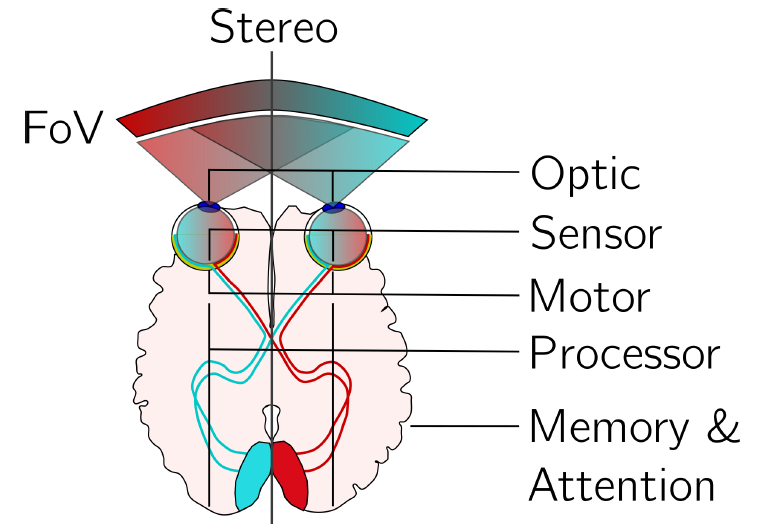
\includegraphics[width=0.5\textwidth]{../../Grafiken/HVS-model_from-star-report.png}
	\caption{Modell des visuellen Wahrnehmungsapparates des Menschen aus \cite{doi:10.1111/cfg.13150}}
	\label{fig::eye01}
\end{figure}
Abbildung \ref{fig::eye01} ist ein Modell des visuellen Wahrnehmungsapparates des Menschen.
Das Modell unterteilt den Sehapparat des Menschen in Optik, Sensorik, Motorik, Verarbeitung, Speicherung und Aufmerksamkeit.
Licht trifft auf die Augen und wird durch die Optik auf die Retina, die Sensorik, weitergeleitet.
Hier wird der visuelle Input abgetastet und gefiltert.
Dabei entstehen zwei Datenströme welche die Verarbeitung stereoskopischer Bilder über einen großen Blickwinkel mit unterschiedlichen räumlich unterschiedlicher Auflösungen ermöglichen.
Die Retina (oder auch Netzhaut) ist mit dem visuellen Kortex verbunden.
Die Signale werden über die visuellen Nerven komprimiert und zum visuellen Kortex transportiert.
Dort werden sie von verschiedenen Bereichen im Gehirn verarbeitet.
Speicherung und Aufmerksamkeit spielen dabei eine wesentliche Rolle.

Das visuelle Wahrnehmungssystem des Menschen hat wesentliche Limitierungen, die bei der Darstellung von Bildern gezielt genutzt werden können.
Die Sehschärfe des ungleich auf der Retina verteilt und nur in in einem kleinen, zentralen Bereich ist die Sehschärfe maximal.
Dieser Bereich wird Fovea oder auch Gelber Fleck genannt.
Je weiter man sich von der Fovea nach außen hin entfernt, desto mehr nimmt die Sehschärfe ab.
Der Bereich um die Fovea ist der periphere Bereich des Auges.
% Eine Verringerung der Bildqualität ist daher im äußeren Bereich möglicherweise nicht wahrnehmbar.
% Diese Eigenschaft motiviert den Versuch, die Bildqualität im peripheren Bereich zu reduzieren, um ohne merkliche Verluste in der visuellen Wahrnehmung des Betrachters den Rechenaufwand des Renderings zu reduzieren.
Das Sichtfeld des visuellen Wahrnehmungsapparates des Menschen ist bei gerade gerichteten Blick horizontal bis circa 190\textdegree{} und mit Augenrotation bis zu 290\textdegree{}.
Visuelle Reize werden über das gesamte Sichtfeld wahrgenommen.
Abhängig von dem zuständigen Bereich auf der Retina gibt es starke Unterschiede, wie die visuellen Reize über das Sichtfeld verteilt, verarbeitet werden.
Durch das Verkleinern (Miosis) und Vergrößern (Mydriasis) der Pupille wird die Menge des einfallenden Lichts in das Auge gesteuert.
Die Pupille nimmt dabei Größen zwischen 2mm und 8mm Durchmesser an.

Die Netzhaut (Retina) ist die photosensitive Schicht des Auges und besteht aus zwei Typen von Photorezeptoren, aus Zapfen und Stäbchen.
Es sind circa $6*10^6$ Zapfen und ungefähr 20 mal so viele Stäbchen auf der Retina verteilt.
Stäbchen sind für die Helligkeitswahrnehmung verantwortlich.
Zapfen sind für die Farbwahrnehmung verantwortlich.
Man unterscheidet zwischen drei Zapfentypen: L-Zapfen für lange Wellenlängen, M-Zapfen für mittlere Wellenlängen und S-Zapfen für kurze Wellenlängen.

Die Fovea ist der Bereich um circa 5,2\textdegree{} um das Zentrum der Retina und besteht fast ausschließlich aus Zapfen.
Die Anzahl der Zapfen nimmt aber nach außen hin stark ab.
Der Bereich von circa 5,2\textdegree{} bis 9\textdegree{} wird als Parafovea bezeichnet.
Der Bereich zwischen circa 9\textdegree{} bis 17\textdegree{} heißt Perifovea.
Fovea, Parafovea und Perifovea sind für die zentrale Sicht verantwortlich.
Alles außerhalb ist die periphere Sicht.
\begin{figure}
	\centering
	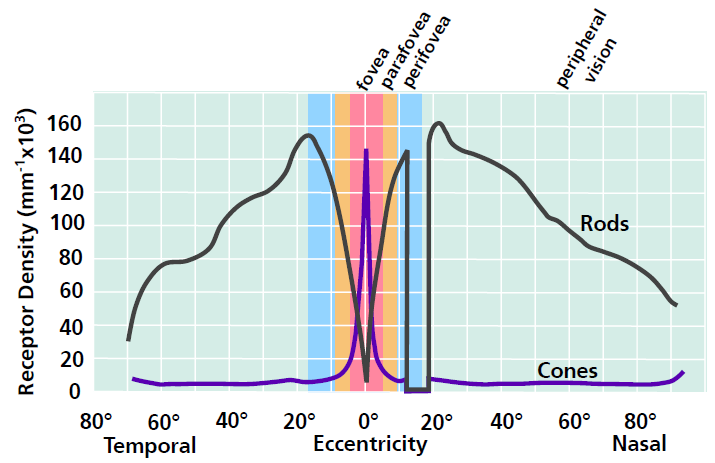
\includegraphics[width=0.5\textwidth]{../../Grafiken/Retinal-photoreceptor-distr_from-star-report.PNG}
	\caption{Verteilung der Photorezeptoren auf der Retina \cite{doi:10.1111/cfg.13150}}
	\label{fig::eye02}
\end{figure}
Abbildung \ref{fig::eye02} zeigt die Dichteverteilung der Photorezeptoren auf der Retina.
Die höchste Dichte der Stäbchen liegt bei circa 15\textdegree{} bis 20\textdegree{} um die Fovea herum.
Ihre Anzahl verringert sich nach außen hin circa linear.
Zapfen und Stäbchen sind sehr unterschiedlich auf der Reitna Verteilt.
Beide folgen aber einem Poisson-Disc Verteilungsmuster.
Die Dichte der Zapfen ist direkt mit der Sehschärfe verknüpft.
Daher fällt die Sehschärfe auch nach außen hin stark ab.
Bei 6\textdegree{} weg vom Zentrum beträgt die Sehschärfe schon nur noch ein Viertel der maximalen Sehschärfe.
Die Sehschärfe hängt aber auch von der Kontraststärke der visuellen Reize ab.
Dabei ist die Kontrastsensitivität von der Anzahl der auf den Reiz reagierenden neuronalen Zellen abhängig, welche ebenfalls nach außen hin stark abnimmt.
Die Farbsensitivität ist von der Verteilung von Stäbchen und Zapfen abhängig.
Die Zapfen zur Erkennung von grünem und rotem Licht sind vermehrt in der Fovea und eher weniger im peripheren Bereich verteilt.
Von allen Zapfen sind lediglich neun Prozent zur Erkennung von blauem Licht.
Diese sind vermehrt im peripheren Bereich verteilt als im Zentrum.
Rezeptoren im Auge passen sich deutlich schneller an die Helligkeit als an die Dunkelheit an.

Das Auge ist dauerhaft in Bewegung.
Sechs externe Muskeln ermöglichen es verschiedene Objekte von Interesse (OvI) in die Fovea zu bringen und zu fokussieren.
Die wichtigsten Arten von Augenbewegungen sind: Sakkaden, Vestibular-Okularer Reflex, weiche Augenverfolgung (Smooth pursuit eye motion (SPEM)) und (coupled vergence-accommodation motion).
\todo{Englische Begriffe richtig übersetzen.}
Der Vestibular-Okulare Reflex passiert relativ schnell mit einer Latenz von 7ms - 15ms und ermöglicht auch bei schnellen Kopfbewegungen OvI zu fixieren.
Der SPEM ermöglicht die weiche Verfolgung eines sich bewegendes Objektes.
Bei der Wahrnehmung der Umgebung ist die Sakkade und Fixation die wichtigsten Eigenschaften des Auges.
Eine Sakkade bezeichnet das schnelle springen von einem Ovi zu einem anderen.
Dabei erreicht das Auge Geschwindigkeiten von bis zu 900\textdegree/s.
Die Sehsensivität ist während einer solchen Sakkade stark geschwächt (saccade suppression).
Eine Fixation dauert zwischen 100ms - 1.5s.
Sie tritt meist dann auf, wenn ein OvI genauer betrachtet wird und die Augen darauf ruhen.
In natürlichen Szenen treten zwei bis drei Sakkaden pro Sekunde auf, mit jeweils durchschnittlich 250ms Fixationszeit.
Der räumliche Abstand zwischen den Fixierungen beträgt dabei circa 7\textdegree{}.
Ein Abstand von mehr als 30\textdegree{} wird als unangenehm empfunden und hat meist eine Kopfbewegung zur Folge.
Auch während einer Fixierung macht das Auge wichtige kleine Bewegungen, sogenannte Tremor Bewegungen.
Werden diese bewusst unterdrückt, resultiert dies in einem schwindenden Bild.
Kleinere Augenbewegungen von bis zu 2.5\textdegree{}/s haben kaum einen Effekt auf die Sehschärfe.

Das die Fovea einen sehr wichtigen Teil der visuellen Informationen liefert spiegelt sich auch darin wieder, dass über 30 Prozent des primären Sehverarbeitungsbereichs des Gehirns für die zentralen 5\textdegree{} des Sehfeldes, der Fovea, zuständig sind.
Der periphere Bereich ist hier benachteiligt, liefert aber trotzdem einen großen und wichtigen Teil der Informationen.
Besonders für das (frühe) Erkennen von Kontrasten, Objekten und Tieren.
%Farbveränderungen im peripheren Bereich haben einen größeren Einfluss als eine Veränderung der Ausrichtung \todo{Dieser Satz: richtig übersetzt / verstanden? Was heißt "Orientation" hier?}.
Aus dem peripheren Bereich werden auch wichtige kontextuelle Informationen geliefert.
Dies ermöglicht unter Anderem die Vorverarbeitung von Informationen.

Die Aufmerksamkeit spielt eine wichtige Rolle in der Verarbeitung von visuellen Stimuli. % Selective attention, focused attention, divided attention.
Visuelles tunneling bezeichnet das längere Fokussieren auf einen bestimmten Punkt, wodurch ein Großteil der peripheren Informationen nicht mehr oder stark reduziert wahrgenommen werden.
Die visuelle Auflösung reduziert sich circa linear für die ersten 20-30\textdegree{}.
Jedes lineare Modell für das visuelle Wahrnehmungssystem des Menschen ist aber immer nur eine Annäherung.
Farben haben einen großen Einfluss auf die Wahrnehmung von Kontraste.
Die Bewegungserkennung ist sowohl in der Fovea als auch im peripheren Bereich ähnlich oder genauso gut.
\todo{Grundlagen zum menschlichen Sehapparat überarbeiten: Teilweise sind Sätze zusammenhangslos aneinandergereiht. Hier eine bessere Verknüpfung finden.}

\section{Volumenrendering und Transferfunktion}\label{sec::voltff}
Es ist nicht trivial, 3D Volumendaten auf einem 2D Bildschirm informativ zu präsentieren.
In einem Volumen gibt es möglicherweise mehrere für den Betrachter interessante Objekte, welche sich durchaus gegenseitig überdecken können.
Daher stellt sich die Frage, wie die Volumendaten auf dem Bildschirm projiziert werden und dabei für den Betrachter auch Informationen an verschiedenen Positionen innerhalb des Volumen sichtbar gemacht werden können.
Raycasting ermöglicht in Verbindung mit einer Transferfunktion, ein Volumen auf eine 2D Ebene zu projizieren und dabei einzelne Bereiche des Volumens farbig hervorzuheben oder transparent erscheinen zu lassen.

\subsection{Raycasting}\label{sec::rc}
Raycasting ist ein Verfahren um Volumendaten abzutasten und auf eine 2D Rastergrafik zu projizieren.
Wie beim Raytracing werden beim Raycasting auch Sichtstrahlen verfolgt.
Die Sichtstrahlen werden dabei ausgehend von einer virtuellen Kamera im Raum verfolgt.
\begin{figure}[]
	\centering
	\begin{minipage}[b]{0.49\textwidth}
		\centering
		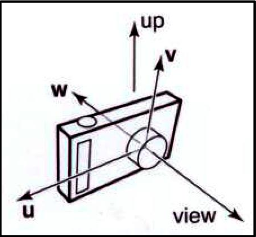
\includegraphics[width=0.5\textwidth]{../../Grafiken/Virtuelle-Kamera.PNG}
		\caption{Illustration einer virtuellen Kamera im Raum \cite{Dr.MichaelKrone2016/2017}}
		\label{fig::rc01}
	\end{minipage}
	\hfill
	\begin{minipage}[b]{0.49\textwidth}
		\centering
		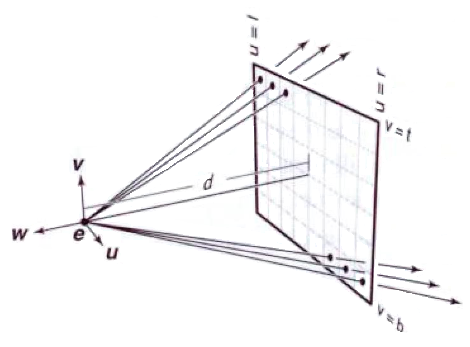
\includegraphics[width=1\textwidth]{../../Grafiken/Virtuelle-Kamera-und-Bildebene.PNG}
		\caption{Illustration der virtuellen Kamera und der Bildebene \cite{Dr.MichaelKrone2016/2017}}
		\label{fig::rc02}
	\end{minipage}
\end{figure}
Die virtuelle Kamera, siehe Abbildung \ref{fig::rc01}, ist im Raum an Position \texttt{e} positioniert, dies ist auch das Projektionszentrum, falls es keine orthogonale Projektion ist.
Die Position \texttt{e} entspricht relativ der Position des Betrachters vor dem Bildschirm.
Mit \texttt{u}, \texttt{v} und \texttt{w} wird die Ausrichtung der Kamera im Raum eindeutig bestimmt.
In einer Entfernung \texttt{d} von \texttt{e} aus in Richtung \texttt{-w} ist die Bildebene \ref{fig::rc02} Positioniert.
Die Größe der Bildebene wird durch \texttt{l}, \texttt{r}, \texttt{b} und \texttt{t} bestimmt.
Abhängig von der Größe des Bildschirms oder der Größe der gewünschten Rastergrafik, wird die Bildebene virtuell in die gewünschte Anzahl an Pixel in die Breite und Höhe unterteilt.
Jeder dieser Teile entspricht nun einem Pixel der Rastergrafik.
Nun kann für jeden Pixel ein Strahl, ausgehend von \texttt{e}, in Richtung des entsprechenden Punktes auf der Bildebene, ausgesendet und verfolgt werden.
\begin{figure}
	\centering
	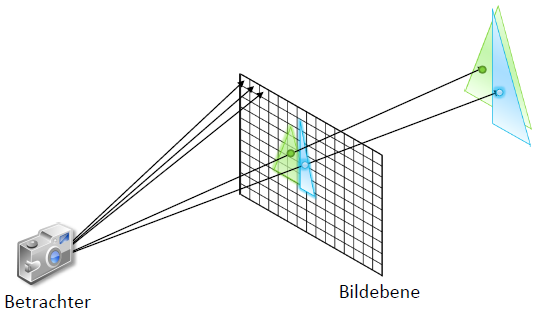
\includegraphics[width=0.5\textwidth]{../../Grafiken/Raytracing.png}
	\caption{Illustration der Projektion von Objekten auf die Bildebene mit Hilfe von Raytracing. \cite{Dr.MichaelKrone2016/2017}}
	\label{fig::rc03}
\end{figure}
Trifft ein Strahl Objekte in der Szene, wird dadurch ein Farbwert ermittelt, den der entsprechende Pixel annehmen kann und und die Szene dadurch auf den Bildschirm projiziert wird.
Siehe auch Abbildung \ref{fig::rc03}.
\todo{Grundlagen zu Raycasting hier. Vektoren als richtige Vektorensymbole darstellen (mit Pfeil oben drauf).}

\subsection{Volumenrendering}
Ein Volumen kann mit Hilfe von Raycasting abgetastet und auf den Bildschirm projiziert werden.
Hier wird wie beschrieben, für jeden Pixel ein Strahl in die Szene gesendet.
Anstelle von verschiedenen Objekten gibt es nun ein Volumen welches aus vielen kleinen Voxeln besteht.
Das Volumen ist ein dreidimensionales Bild, wobei statt 2D Pixel es aus 3D Voxel besteht.
Ein Voxel ist eine Box in dem Volumen, mit einer Position, einer Ausdehnung in drei Dimensionen und einer Dichte.
Wird ein Strahl in das Volumen gesendet, so wird dieser in Intervallen abgetastet.
Für jeden Abtastpunkt kann mit Hilfe einer Transferfunktion ein Farbwert ermittelt werden, welche zusammen einen Farbwert für den Pixel ergeben.
\todo{Anwendung von Raycasting zum Volumenrendering. Illustration von Rayasting und Volumenrendering mit mehreren Raysamples einfügen.}

\subsection{Transferfunktion}
Die Transferfunktion ist ein mächtiges Werkzeug für die Visualisierung von Volumendaten.
Mit Hilfe einer Transferfunktion können bestimmte Bereiche des Volumen verschieden stark ausgeblendet, oder auch farbig dargestellt werden.
Die Transferfunktion bestimmt für einen Voxel, abhängig von seiner Dichte, einen Farb- und Opazitätswert.
Dadurch können zum Beispiel Strukturen innerhalb des Volumens mit einer hohen Dichte farbig und kräftig hervorgehoben werden.
Strukturen mit einer geringeren Dichte können transparent und weniger farblich dargestellt werden.
\todo{Funktion der Transferfrunktion im Volumenrendering erläutern. Unter Umständen ein Beispiel Bild mit einer Anwendung der Transferfunktion verwenden.}

\section{Eyetracking}\label{sec::eyetr}
% \todo{Was ist Eyetracking?}
Für einige wahrnehmungsorientierte Methoden ist es notwendig, den aktuellen Blickpunkt des Betrachters auf dem Bildschirm zu wissen und daher die Augenaktivitäten zu messen.
In diesem Zusammenhang fällt meistens der Begriff \texttt{Eyetracking}.
Aber was ist Eyetracking?
Eyetracking ist das Messen von Augenaktivitäten eines Betrachters.
In der Regel betrachtet der Betrachter dabei einen Bildschirm während seine Augenaktivität gemessen werden, wodurch Informationen über den Blickverlauf und die Fixationsdauer bestimmter Punkte auf diesem Bildschirm errechnet werden können.
Diese Informationen ermöglichen es, Rückschlüsse über das betrachtete Bild zu ziehen, wie zum Beispiel, welche Objekte eines Bildes besonders interessant für den Betrachter sind.
Eyetracking ermöglicht aber nicht nur das Messen von Daten um diese im Nachhinein auszuwerten, sondern auch das Nutzen solche Daten für interaktive Anwendungen in Echtzeit.
Da in dieser Arbeit ein externer Tobii Eye Tracker verwendet wurde, beziehen sich folgende Informationen hauptsächlich aber nicht ausschließlich auf Tobii Eyetracker.
Die Firma Tobii AB schreibt auf ihrer Webseite zum Thema: Was ist Eyetracking?, dass Eye Tracking eine Technologie ist, die es ermöglicht, ein Gerät durch die natürliche Bewegung der Augen zu steuern \cite{tobii}.
\begin{figure}
	\centering
	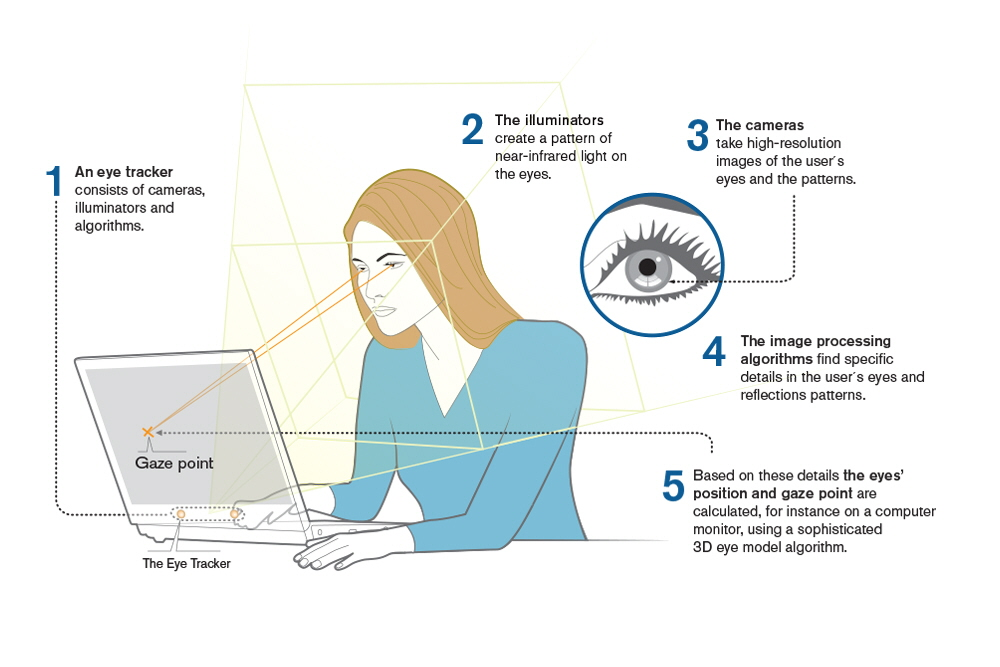
\includegraphics[width=1\textwidth]{../../Grafiken/How-20DoesEyetrackingWork_ScreenBased.jpg}
	\caption{Illustration der Funktionsweise von Tobii Pro Eyetracker. \cite{tobiipro}}
	\label{fig::et01}
\end{figure}
Dabei werden vier grundlegende Bestandteile des Eye Tracking, wie die Firma Tobii AB es realisiert, genannt.
In der Regel benötigt man für das Messen von Augenaktivitäten zwei grundlegende Dinge, die auch in Abbildung \ref{fig::et01} abgebildet sind: Eine Lichtquelle (2) und eine Kamera (3).
Es gibt verschiedene Möglichkeiten, die Augenaktivitäten zu messen.
Die am häufigsten genutzte Technik, welche auch von den Tobii Eyetrackern genutzt wird, ist \texttt{Pupil Centre Corneal Reflection (PCCR)}.
Die Lichtquellen sind dabei auf die Augen gerichtet und erzeugen auf ihnen ein spezielles Reflektionsmuster.
Die Kamera des Eyetrackers (3) nimmt mit einer hohen Abtastrate Bilder der Augen und ihrer Reflektionsmuster auf.
Nun können spezielle Bildverarbeitungsalgorithmen (4) auf die erfassten Daten angewendet werden und die Reflektionspunkte auf den Bildern bestimmt werden.
Anhand dieser Punkte und eines Modells des Auges kann die Blickrichtung der Augen, die Position der Augen im Raum und die Blickpunkte der Augen auf dem Bildschirm berechnet werden (4 + 5).
% \todo{Wie werden die Augen getrackt?}
% \todo{Wie sehen Messwerte aus und wie verwendet man sie richtig (Koordinatensysteme, Bildschirm und Fensteroffset.)}

\begin{figure}[]
	\centering
	\begin{minipage}[b]{0.49\textwidth}
		\centering
		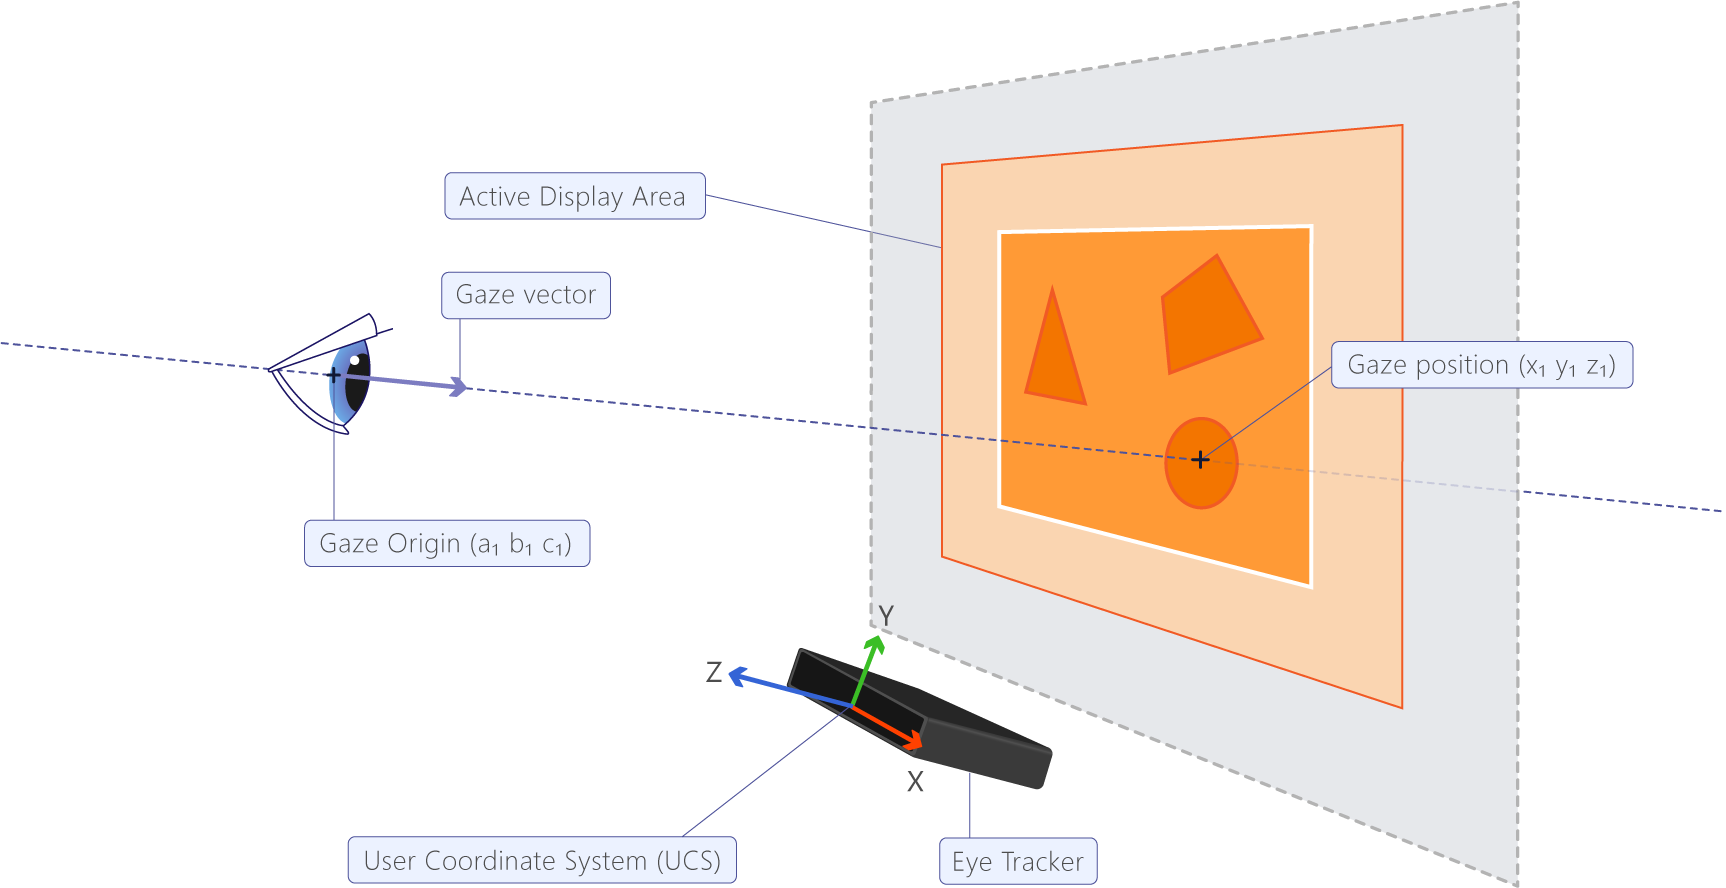
\includegraphics[width=1\textwidth]{../../Grafiken/UCS.png}
		\caption{Nutzer Koordinatensystem \cite{tobiisdk}}
		\label{fig::et02}
	\end{minipage}
	\hfill
	\begin{minipage}[b]{0.49\textwidth}
		\centering
		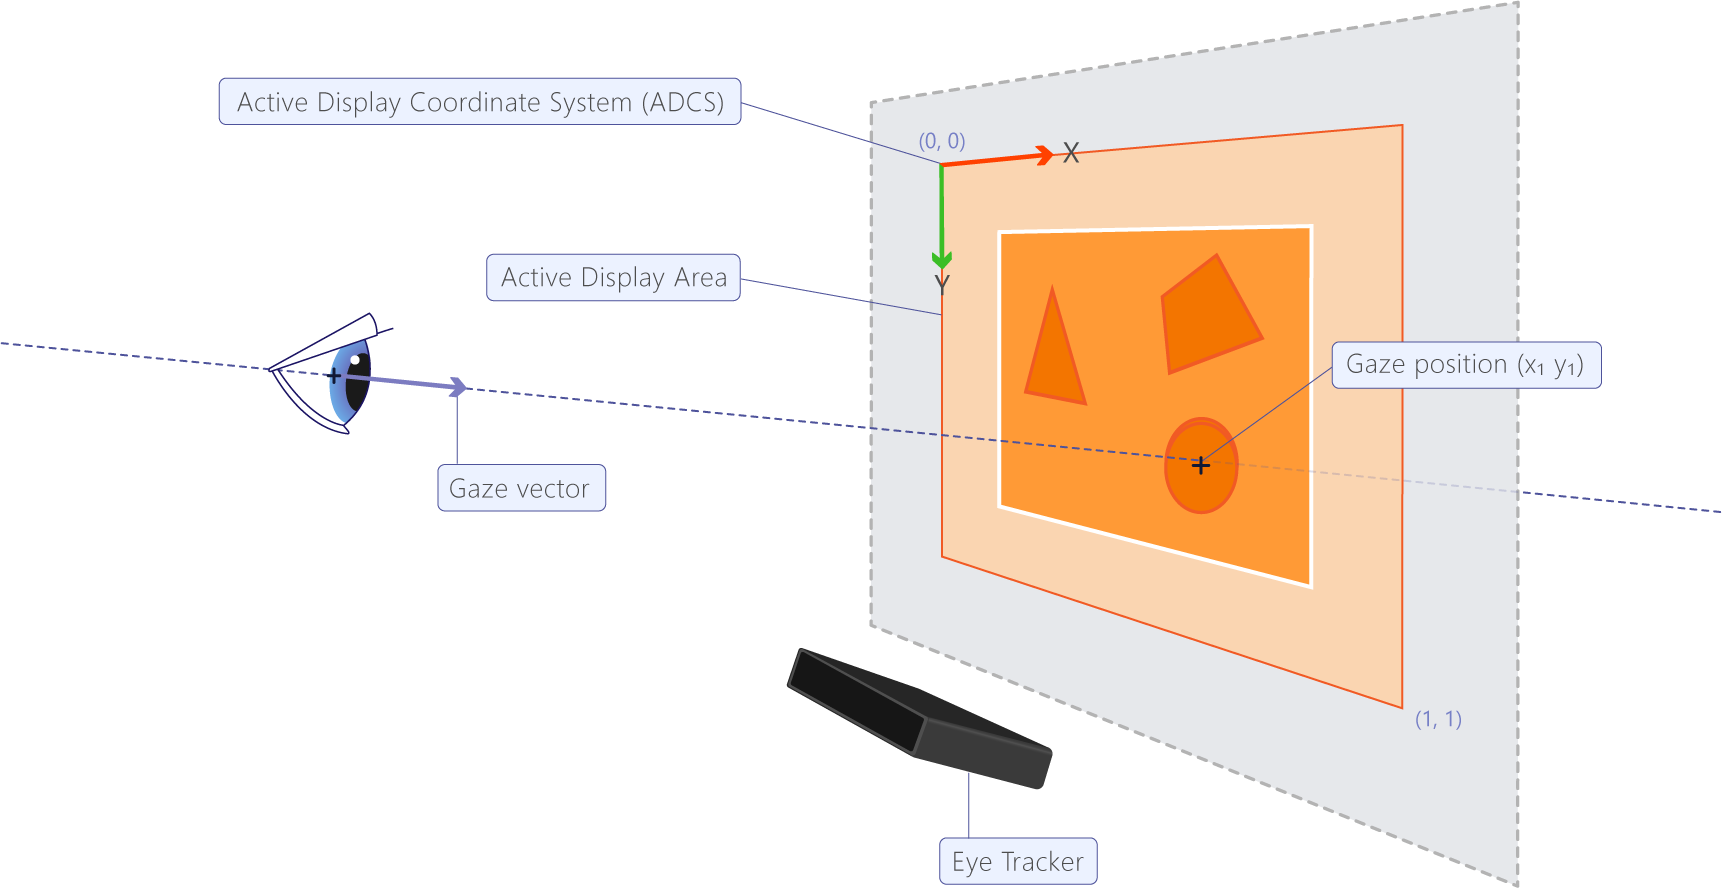
\includegraphics[width=1\textwidth]{../../Grafiken/ADCS.png}
		\caption{Aktives Display Koordinatensystem \cite{tobiisdk}}
		\label{fig::et03}
	\end{minipage}
\end{figure}
Die Position eines Auges im Raum wird als \texttt{Gaze origin} bezeichnet und wird bei Tobii Pro Eyetrackern im Nutzer Koordinatensystem angegeben, siehe Abbildung \ref{fig::et02}.
Der Blickpunkt des Auges auf dem Bildschirm ist in der Regel das, was von größtem Interesse ist und wird als \texttt{Gaze point} bezeichnet.
Der \texttt{Gaze point} wird im Aktiven Display Koordinatensystem angegeben, siehe Abbildung \ref{fig::et03}.
Dieses Koordinatensystem hat den Ursprung an der Position oben links des aktiven Bildschirmbereichs, und der Punkt (1,1) ist an der Position rechts unten des aktiven Bildschirmbereichs.
Die Umrechnung in Bildschirmkoordinaten funktioniert durch die Multiplikation mit der Breite und Höhe des Bildschirms in Pixel.
Die Koordinaten sind dann relativ zu dem aktiven Display.
Dieses Display muss nicht unbedingt das einzige Display sein.
Werden mehrere Bildschirme verwendet, muss möglicherweise ein Offset auf die Werte gerechnet werden, um die richtigen Bildschirmkoordinaten für den Bildschirm, auf dem die Anwendung dargestellt wird, zu erhalten.

%\todo{Umrechnung in Pixel und bei mehreren Bildschirmen.}
In Abschnitt \ref{sec::eye} wurden verschiedene Arten von Augenbewegungen angesprochen.
Eine sehr wichtige Rolle spielen dabei Fixationen und Sakkaden.
Bei der Analyse der visuellen Wahrnehmung des Menschen ergeben die Daten der Fixationen wichtige Informationen über Eigenschaften des visuellen Stimuli.
Bei einer Fixation fixieren die Augen einen gewissen Punkt für eine vergleichsweise lange Zeit (100ms - 1.5s) und können dadurch viele Informationen des fixierten Objekts erfassen.
Sakkaden hingegen sind kurze (20ms - 40ms) und schnelle Augenbewegungen zwischen zwei Fixationen.
Für wahrnehmungsorientierte interaktive Anwendungen ist es daher wichtig, eine hohe Abtastrate und niedrige Latenz bei der Erfassung der Augenaktivitäten zu haben.
Dies ermöglicht es, schnell zwischen einer Sakkade und Fixation zu unterscheiden und das nächste Bild, ohne eine merkbare Verzögerung und entsprechend des neuen Blickpunktes, darzustellen.
So sollte bei der Methode des wahrnehmungsorientierten Renderings, wobei nur in dem fovealen Bereich das Bild mit hoher Auflösung dargestellt wird, ein Update ca. zwischen 5ms bis 60ms nach der Augenbewegung gestartet worden sein, um eine Bildveränderung nicht zu bemerken.
Diese Zeit ist dabei abhängig davon, wie weit die unscharfe Fläche von der Fovea entfernt ist \cite{doi:10.1111/cgf.13150}.
%\begin{figure}
%	\centering
%	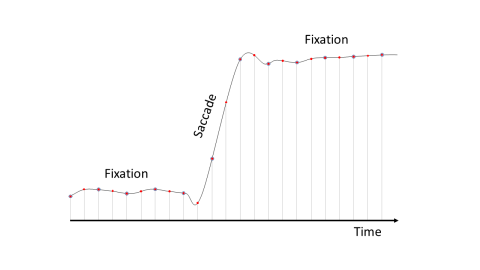
\includegraphics[width=0.5\textwidth]{../../Grafiken/Sampling-20frequency-201.png}
%	\caption{Abtastrate einer typischen Augenbewegung \cite{tobiisdk}}
%	\label{fig::et04}
%\end{figure}

Der in dieser Arbeit verwendete Tobii Pro Eyetracker hat eine Abtastfrequenz von 600 Hz.
Dies entspricht einem Abtastintervall von 1.67ms und ist vergleichsweise zu anderen aktuellen Eyetrackern recht hoch.
Diese haben oft eine Abtastfrequenz von 60 Hz oder 120 Hz.
Geräte mit Abtastraten im Frequenzbereich von 600 Hz und höher sind ausreichen schnell um Sakkaden messen zu können und haben eine entsprechend niedrige Latenz, welche es ermöglicht, eine Bildveränderung nicht wahrzunehmen.
\todo{Genaue Technische Daten des verwendeten Tobii Pro Eyetrackers nachschauen.}
Hohe Abtastraten heißt aber auch viele Daten pro Sekunde.
Für die Anwendung in dieser Arbeit ist es wichtig, den aktuellsten Blickpunkt des Auges zu kennen.
Daher wird der letzte gemessene gaze point des Eyetrackers für das Berechnen des nächsten Bildes verwendet.
Ein weiteres Problem bei vielen Messdaten ist es auch, dass es mehr fehlerhafte Messdaten gibt.
Die Daten, die über die Tobii Pro SDK durch den Eyetracker geliefert werden, enthalten dafür einen Validity Code.
Dieser Wert gibt an, ob eine Messung mit hoher Wahrscheinlichkeit richtige Daten enthält, oder nicht.
Dadurch können wahrscheinlich fehlerhafte Daten früh abgestoßen werden.
% \todo{Messgeschwindigkeit vs Augengeschwindigkeit}
% \todo{Validity Codes}
% \todo{Vorherige Todos ausschreiben und ggf. mehr.}

\section{GPU Architektur}\label{sec::gpuarc}
Ein wichtiger Faktor, wenn es um interaktive Anwendungen geht, ist die Performanz.
Viele Algorithmen haben essentielle Bestandteile welche ihre Komplexität nach unten beschränken.
Die Einführung von Parallelität ist ein wichtiger Ansatz, um die Performanz von Anwendungen beziehungsweise ihrer Algorithmen weiter zu verbessern.
Gerade Algorithmen in der Bildberechnung und -Verarbeitung eignen sich besonders um diese zu parallelisieren.
In der Bildverarbeitung werden viele gleiche Berechnungen auf unterschiedlichen Daten ausgeführt.
Graphics Processing Units (GPUs) oder auch Grafikkarten sind für diese Art von Berechnungen optimiert.
\begin{figure}
	\centering
	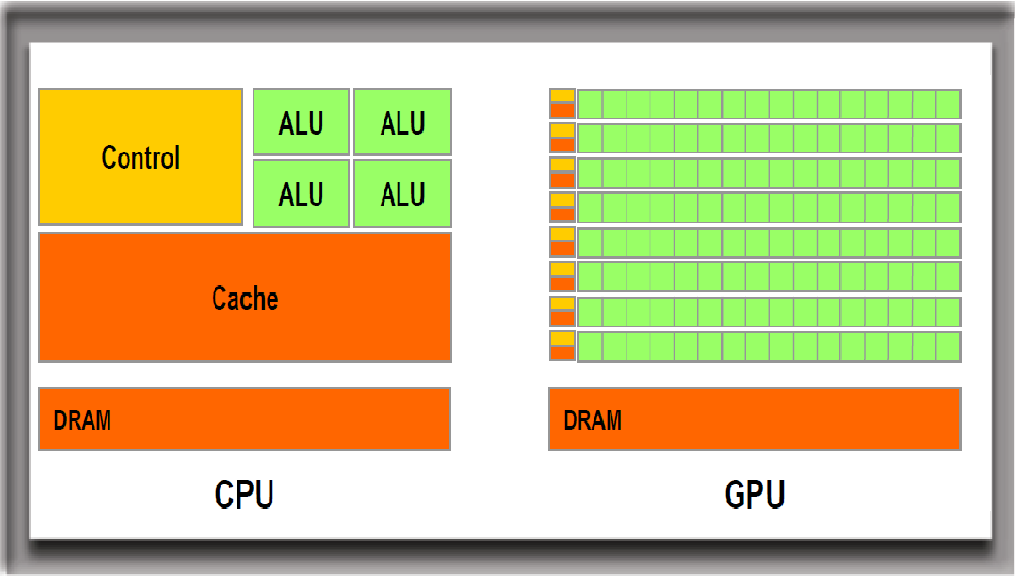
\includegraphics[width=0.5\textwidth]{../../Grafiken/CPU-GPU-Structures1.png}
	\caption{CPU vs. GPU. \url{http://www.keremcaliskan.com/wp-content/uploads/2011/01/CPU-GPU-Structures1.png}}
	\label{fig::ga01}
\end{figure}
% GPU vs CPU
Im Vergleich zu Central Processing Units (CPUs) besitzen GPUs eine deutlich höhere Anzahl an Prozessoren, siehe Abbildung \ref{fig::ga01}.
Aktuell besitzen Prozessoren meist vier oder acht Rechenkerne und eine Taktfrequenz von ca. 4 Ghz.
GPUs hingegen haben mehrere tausend Berechnungseinheiten die gleichzeitig Berechnungen durchführen können, dafür aber bei ca. einem drittel der Taktfrequenz von CPUs.

Fast jeder Computer besitzt heutzutage hochparallele Einheiten, meist eine GPU.
In den Anfängen waren GPUs sehr eng mit grafischen Berechnungen verbunden um die Berechnung von Farbwerten von Pixeln zu beschleunigen.
Heute werden GPUs zur Beschleunigung von fast beliebigen Anwendungen genutzt.
Programmierschnittstellen wie OpenCL oder CUDA ermöglichen die Nutzung von GPUs für allgemeine Berechnungen, oder auch General Purpose Computation on Graphics Processing Unit (GPGPU).

\subsection*{OpenCL}
OpenCL (Open Computing Language) ist ein Standard für das allgemeine Programmieren für parallele CPU oder GPU-Platformen.
Dabei stellt OpenCL eine Programmierschnittstelle für das koordinieren paralleler Berechnungen auf unterschiedlichen Platformen zur Verfügung, sowie eine Programmiersprache für die eigentliche Programmierung von Programmen, die auf parallelen Platformen wie einer GPU ausgeführt werden sollen.

Eine OpenCL Anwendung ist die Kombination des Codes eines Programms, das auf dem Host und den OpenCL Devices ausgeführt wird.
Der Host ist dabei der Teil der Anwendung, der mit dem OpenCL Kontext über die OpenCL API kommuniziert.
Ein Kontext ist die Umgebung, in der ein OpenCL Kernel ausgeführt wird und weitere Eigenschaften definiert sind.
Der Kernel ist eine Funktion die in einem OpenCL Programm geschrieben wurde und durch ein OpenCL Device ausgeführt wird.
Ein Device entspricht meistens eine GPU oder CPU, die OpenCL implementiert. % bzw. deren Treiber OpenCL implementieren

\subsubsection*{OpenCL Platform Modell}
\begin{figure}
	\centering
	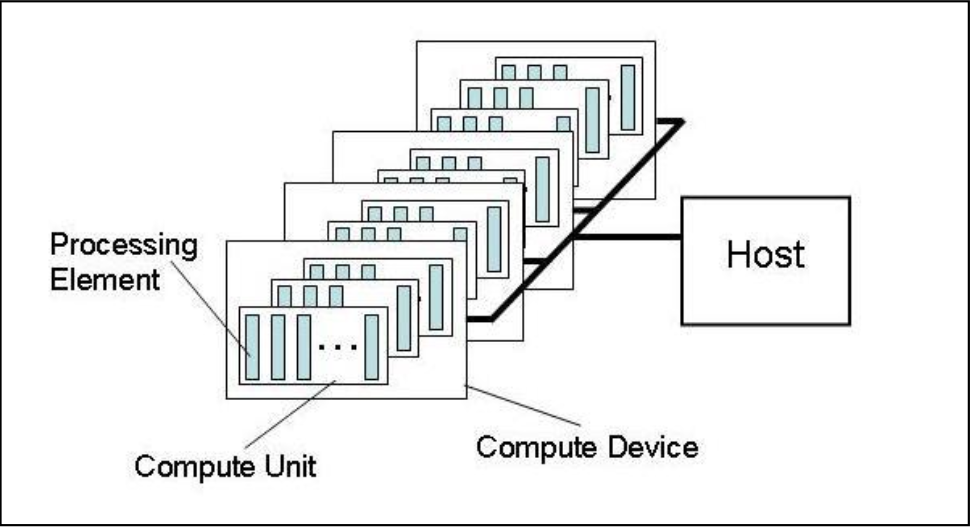
\includegraphics[width=0.5\textwidth]{../../Grafiken/OpenCL_PlatformModel.png}
	\caption{OpenCL Platform Modell ... ein Host, mehrere Compute Devices (ein Compute Device entspricht zum Beispiel einer GPU) mit je einer oder mehreren Compute Units. \url{https://www.khronos.org/registry/OpenCL/specs/opencl-2.1.pdf}}
	\label{fig::ga02}
\end{figure}
Das Platform Modell von OpenCL ist eine Abstraktion davon, wie OpenCL die Hardware sieht.
Die Beziehung zwischen seinen Einheiten und der Hardware ist dabei größtenteils von der verwendeten Hardware und ihrer Implementierung von OpenCL abhängig.
Es besteht aus einem Host, welcher mit ein oder mehreren Devices verbunden ist.
Diese sind unterteilt in Compute Units (CUs), welche weiter in Processing Elements (PEs) unterteilt sind.
Berechnungen auf einem solchen Device werden in Processing Elements ausgeführt.
Die Host-Anwendung gibt den Start des Kernel-Codes in Auftrag.
Das OpenCL Device führt dann den Kernel Code auf den Processing Elements des Devices aus und hat dabei eine große Freiheit darüber, wie die Berechnungen auf den Processing Elements abgebildet werden.
Falls die Processing Elements innerhalb einer Compute Unit die gleiche Folge von Befehlen ausführen, bezeichnet man ihren Befehlsfluss als konvergiert, sonst als divergiert.

\subsubsection*{OpenCL Ausführungsmodell}
Der Host kann über Funktionen der OpenCL API mit einem Device über eine Command-Queue interagieren.
Eine Command-Queue ist mit maximal einem Device verknüpft.
Über die Command-Queue können Befehle zum starten eines Kernels, Transferieren von Daten zwischen Host und Device und Befehle zur Synchronisation ausgeführt werden.
Ein Befehl durchläuft dabei immer sechs Zustände: Queued (Eingereiht), Submitted (Übermittelt), Ready (Bereit), Running (Ausführend), Ended (Beendet) und Complete (Abgeschlossen).
Wird ein Kernel für die Ausführung übermittelt, wird für diesen ein Index-Raum definiert.
Der Kernel selbst, die zugehörigen Parameter und die Parameter, die seinen Index-Raum definieren, definieren eine Kernel Instanz.
Wird eine Kernel Instanz auf dem Device ausgeführt, wird für jeden Punkt in seinem Index-Raum eine Ausführung des Kernels gestartet.
Eine solche Ausführung wird Work-Item genannt.
Work-Items, die zu einer bestimmten Kernel Instanz gehören, werden von dem Device in Gruppen gehandhabt.
Diese Gruppen heißen Work-Groups.

\begin{figure}
	\centering
	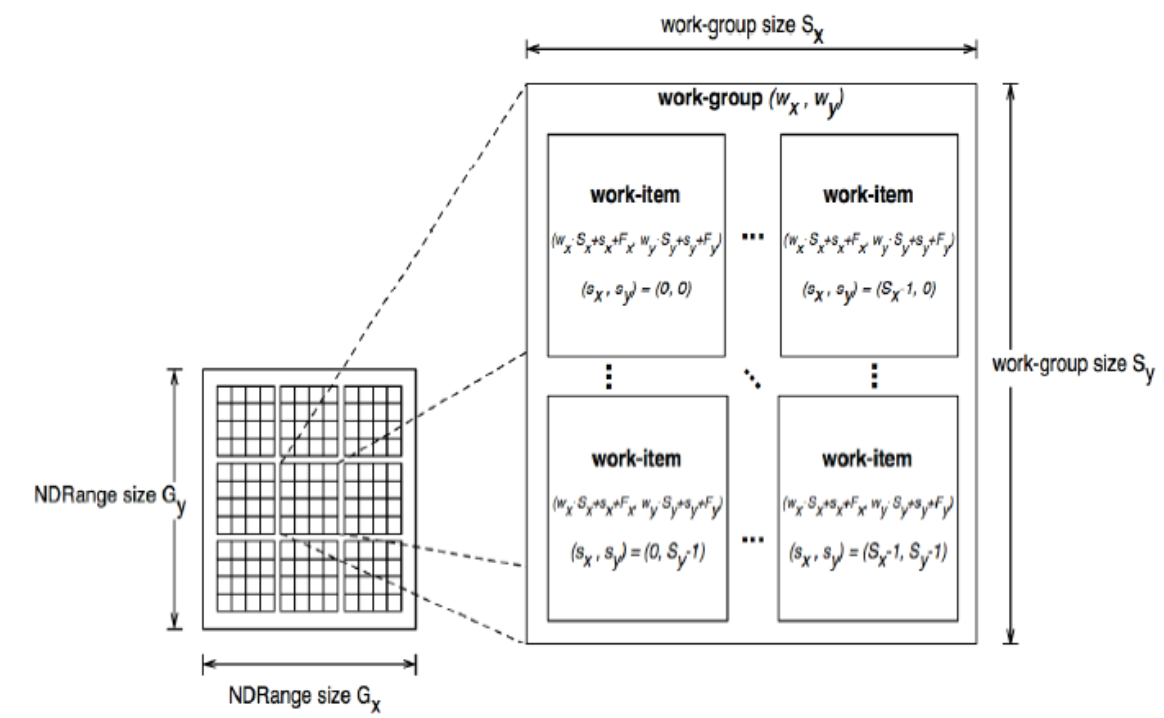
\includegraphics[width=0.75\textwidth]{../../Grafiken/OpenCL-NDRange-Mapping.png}
	\caption{OpenCL NDRange-Mapping mit 2 Dimensionen. \url{https://www.khronos.org/registry/OpenCL/specs/opencl-2.1.pdf}}
	\label{fig::ga03}
\end{figure} 
Der Index-Raum ist durch eine NDRange definiert.
Dies ist ein N-dimensionaler Index-Raum, wobei N die Werte 1, 2 oder 3 annehmen kann.
Eine NDRange wird dementsprechend durch drei Integer-Arrays der Länge N definiert: Die Ausdehnung des Index-Raums, ein Offset der Indices an dem sie starten und die Größe der Work-Groups, jeweils in N Dimensionen.

Jedes Work-Item hat ein N-Dimensionales Tupel, welches seine globale ID repräsentiert.
Work-Groups erhalten ebenfalls N-Dimensionale Tupel als ID.
Die Anzahl von Work-Groups ist abhängig von der definierten Größe von Work-Groups und der Größe des Index-Raums.
Work-Items sind je einer Work-Group zugewiesen und haben eine loakle ID innerhalb ihrer Work-Group.
Dadurch sind Work-Items eindeutig auf zwei verschiedene Arten definiert: Durch die globale ID beziehungsweise den globalen Index und durch die ID ihrer Work-Group zusammen mit ihrer lokalen ID in dieser Work-Group.

Wird die Ausführung einer Kernel-Instanz gestartet, werden die damit assoziierten Work-Groups in einen Work-Pool platziert und sind damit ausführungsbereit.
Das Device entnimmt aus dem Work-Pool nach und nach Work-Groups und führt ein oder mehrere gleichzeitig aus.
Da die Work-Groups aus dem Work-Pool in jeglicher Reihenfolge ausgeführt werden können, gibt es keinen sicheren Weg, verschiedene Ausführungen von Work-Groups zu synchronisieren.

\subsubsection*{Hardware Mapping}
\begin{figure}[]
	\centering
	\begin{minipage}[b]{0.49\textwidth}
		\centering
		\includegraphics[width=1\textwidth]{../../Grafiken/Ausführungsmodell-GPU-Architektur.png}
		\caption{Ausführungsmodell NVIDIA GPU Architektur. \url{http://www.icl.utk.edu/~luszczek/teaching/courses/fall2016/cosc462/pdf/GPU_Fundamentals.pdf}}
		\label{fig::ga04}
	\end{minipage}
	\hfill
	\begin{minipage}[b]{0.49\textwidth}
		\centering
		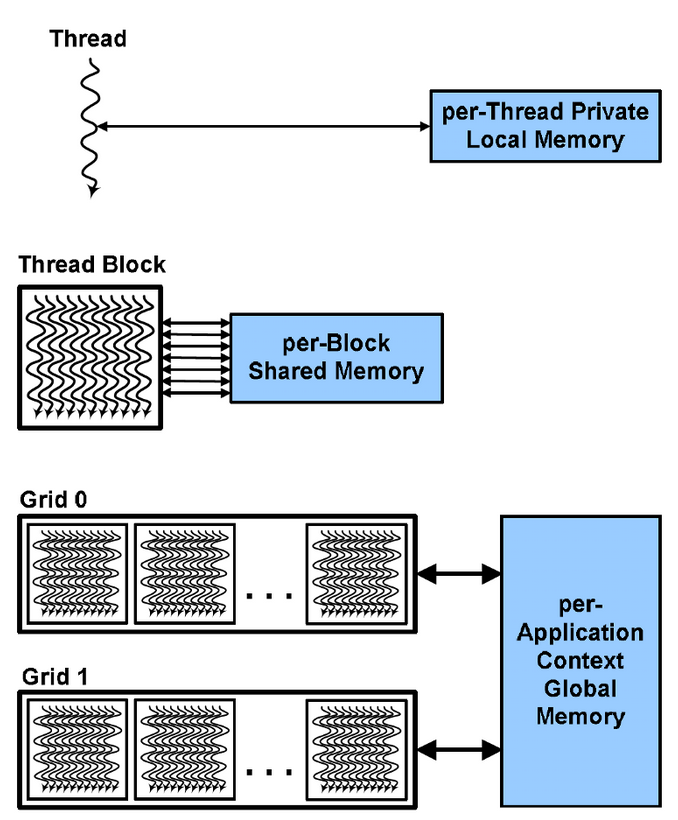
\includegraphics[width=1\textwidth]{../../Grafiken/GPU-Memory-Hierarchie-with-Threads.PNG}
		\caption{CUDA Thread- und Speicher Hierarchie. \url{https://www.nvidia.com/content/PDF/fermi_white_papers/NVIDIA_Fermi_Compute_Architecture_Whitepaper.pdf}}
		\label{fig::ga05}
	\end{minipage}
\end{figure}
\todo{Ausrichtung der Bilder. Links in Fußnote oder Referenzen verschieben.}

In der GPU Architektur gibt zwei große Konzepte, globalen Speicher und Streaming Multiprozessoren (SM).
Globaler Speicher auf der GPU ist analog zu RAM für die CPU.
Auf diesen kann von den Recheneinheiten der GPU und auch durch die Host-Anwendung auf der CPU zugegriffen werden. 
Eine GPU hat mehrere Streaming Multiprozessoren.
Streaming Multiprozessoren führen die eigentlichen Berechnungen aus und haben je eigene Control Units, Register (lokaler Speicher), Ausführungs Pipelines und Caches.
Ein Streaming Multiprozessor besitzt viele Skalare Recheneinheiten, die ähnlich zu einer ALU Berechnungen ausführen.

Im GPU Ausführungsmodell werden Threads von Skalaren Prozessoren ausgeführt.
Ein Thread Block ist eine Gruppe von Threads und wird auf einem Multiprozessor ausgeführt.
Dabei werden Threads innerhalb eines Thread Blocks ausschließlich innerhalb eines Multiprozessors ausgeführt.
Es könnenn aber auch mehrere Thread Blöcke gleichzeitig auf einem Multiprozessor ausgeführt werden.
Dies ist aber durch die verfügbaren Ressourcen limitiert.

Ein Thread Block besteht meistens aus 32-Threads und wird in einer NVIDIA Architektur Warp und in einer AMD Architektur Wavefront genannt.
Ein solcher Thread Block wird physisch parallel auf einem Multiprozessor als Single Instruction Multiple Thread (SIMT) Ausführung ausgeführt.
Die Ausführung eines Thread Blocks wird durch einen (Warp- / Thread-Block) Scheduler geregelt.
Da Threads innerhalb eines Thread Blocks differenziert werden können, ermöglicht dies eine Single Instruction Mutlitple Data (SIMD) Ausführung.
Ein Programm (Kernel) auf der GPU wird als Gitter aus Thread Blöcken gestartet.

OpenCL sieht die Hardware aus abstrakter Sicht und die exakte Beziehung des Platform Modells zu der Hardware wird von OpenCL nicht festgelegt.
Das Platform Modell besteht aus einem Host, OpenCL Devices mit je mehreren Compute Units die jeweils ein oder mehreren Processing Elements enthalten.
In der Realität entspricht der Host in der Regel dem Teil der Anwendung, der auf der CPU ausgeführt wird.
Das OpenCL Device entspricht meist einer GPU und eine Compute Unit kann als Streaming Multiprozessor gesehen werden wobei die Processing Elements dementsprechend den Skalaren Prozessoren innerhalb eines Multiprozessors entsprechen.

Nach OpenCL entspricht eine Work-Group einer Menge von verwandten Work-Items, die alle innerhalb der selben Compute Unit arbeiten.
Ein Work-Item kann von einem oder mehreren Processing Units als Teil einer Work-Group verarbeitet werden.
Sie führen die selbe Kernel Instanz aus und haben gemeinsamen lokalen Speicher und Work Group Funktionen.
Daher ist es naheliegend, das Work-Groups in Thread Blöcke unterteilt werden und alle Thread-Blöcke einer Work-Group auf dem selben Streaming Multiprozessor ausgeführt werden.
In OpenCL können Work-Groups weiter in Sub-Groups unterteilt werden.
Eine OpenCL Sub-Group ist eine implementationsabhängige Gruppierung von Work-Items innerhalb einer Work-Group.
Diese sind eindimensional und haben, bis auf die letzte Sub-Group einer solchen Unterteilung, alle dieselbe Größe.
Es ist ebenfalls naheliegend, dass eine solche Sub-Group einem Thread block entspricht.

Threads innerhalb eines Thread Blocks können also ausschließlich die selben Instruktionen ausführen.
Müssen einige Threads innerhalb eines Thread Blocks aufgrund ihrer ID unterschiedliche Statements ausführen, resultiert dies darin, dass unter Umständen der gesamte Block alle Statements ausführt und am Ende der Berechnung die richtigen Ergebnisse auswählt.
\todo{Quelle dafür}
Dies hat zur Folge, dass ein Thread Block der divergiert deutlich längere Ausführungszeiten hat, als ein konvergierender Thread Block.
Bei der Implementierung eines OpenCL Kernels kann eine geschickte Strukturierung des Codes daher das gleiche Ergebnis mit besserer Performanz generieren.

Die Wahl der Work-Group Größe ist ebenfalls wichtig.
Da Thread Blöcke aktuell meist eine Größe von 32 Threads besitzen und unter der Annahme, dass Work-Groups in Thread Blöcke unterteilt werden, macht es Sinn, die Größe einer Work-Group als vielfaches von 32 zu wählen.
Ansonsten kann es passieren, dass Thread Blöcke zur Ausführung gestartet werden, bei denen eine große Anzahl an Threads kein Teil der Berechnung sind und Ressourcen dadurch verschwendet werden.

\begin{figure}
	\centering
	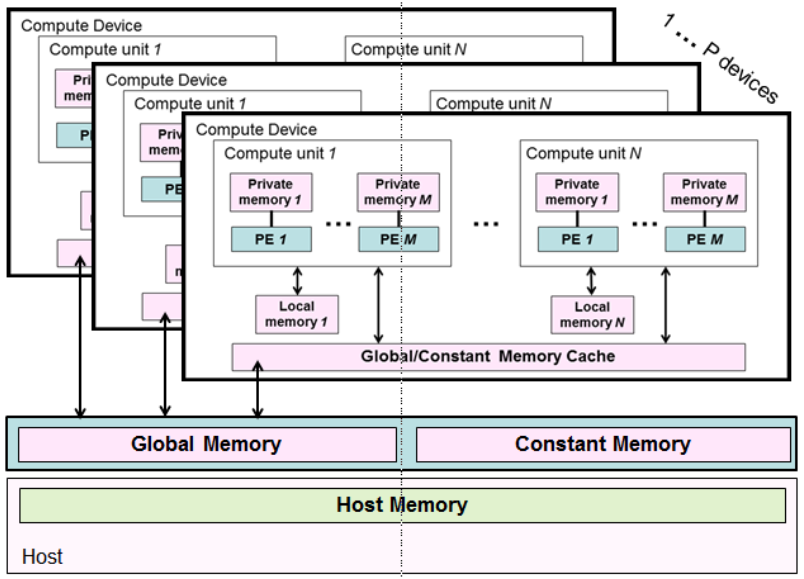
\includegraphics[width=0.5\textwidth]{../../Grafiken/OpenCL-Memory-Model.PNG}
	\caption{OpenCL Speicher Modell \url{https://www.khronos.org/registry/OpenCL/specs/opencl-2.1.pdf}}
	\label{fig::ga06}
\end{figure} 
Ein weiteres Problem sind Speicher Konflikte bei der Ausführung eines Kernels.
Lokaler Speicher von Multiprozessoren ist in Speicher Bänke unterteilt.
Versuchen Threads eines Thread Blocks auf verschiedene Adressen innerhalb der selben Speicher Bank zuzugreifen, entstehen Speicher Konflikte, da eine Speicher Bank nur eine ihrer Adressen gleichzeitig adressieren kann.
Ausführungen eines Thread Blocks mit Speicher Konflikten müssen serialisiert werden und dauern daher deutlich länger.
Eine Ausnahme ist es, falls die Threads eines Blocks alle auf dieselbe Adresse innerhalb einer Speicher Bank lesend zugreifen.
In diesem Fall wird der gelesene Wert an alle Threads gleichzeitig übertragen.
\todo{Quellen einfügen.}
\todo{Bilder Referenzieren.}

%Hier wird der Hauptteil stehen.
%Falls mehrere Kapitel gewünscht, entweder mehrmals \texttt{\textbackslash{}chapter} benutzen oder pro Kapitel eine eigene Datei anlegen und \texttt{ausarbeitung.tex} anpassen.

%LaTeX-Hinweise stehen in \cref{chap:latextipps}.

%noch etwas Fülltext
%\blinddocument

% Entwurf
% Entwurf: Projekt, Raytracer, (Auswahl des) Eyetracker, Vorüberlegungen zur Umsetzung / Integration, Grundidee zur Umsetzung
% Entwurfsziele an die Umsetzungs
\chapter{Entwurf}\label{chap::design}
Die Implementierung dieser Arbeit beruht auf einem Visual Studio Projekt zum Volumen Rendering von Valentin Bruder.
Der erste Abschnitt des Entwurfskapitels beinhaltet den Ausgangspunkt der Implementierung dieser Arbeit in Form einer Beschreibung des ursprünglichen Projekts.
Dies umfasst die allgemeine Architektur der Anwendung und die Umsetzung des Volumenrenderings durch eine Implementierung eines Raycasters als OpenCL Kernel.
Der zweite Abschnitt des Kapitels umfasst Überlegungen für die Erweiterung des Projektes, bezüglich des Ausgangspunktes wie er im ersten Abschnitt beschrieben wurde und dem Ziel dieser Arbeit, sowie die daraus entstandenen Arbeitspakete und die Ansätze für ihre Integration in das bestehende Projekt.

\section{Projekt}\label{sec::proj}
% Qt
Das Visual Studio Projekt, welches als Ausgangspunkt dient, ist eine auf Qt basierende Anwendung.
Qt ist ein vollständiges Cross-Platform Softaware Development Framework, welches in c++ entwickelt wurde, und ermöglicht die einfache Erstellung von Anwendungen mit Benutzeroberflächen und bietet außerdem eine Vielzahl von Bibliotheken, die für eine leichtere und schnellere Entwicklung von Programmen genutzt werden können.

% Struktur von Qt
Die Hauptelemente für die Qt Benutzeroberfläche sind Qt Widgets.
Widgets können Daten darstellen und Nutzereingaben erkennen.
Außerdem stellt ein Widget selbst ein Container für weitere Widgets dar, welche in diesem gruppiert werden.
Innerhalb eines Widgets können Elemente platziert werden, welche Informationen, mögliche Operationen oder Nutzereingaben repräsentieren.
Für die bequeme Erstellung der grafischen Oberfläche bietet Qt die Anwendung Qt Designer.
Der Qt Designer ermöglicht es, Widgets und andere Bausteine der grafischen Oberfläche per Drag und Drop anzuordnen.
Die durch den Qt Designer definierte Oberfläche kann abgespeichert werden und wird von Qt verwendet, um eine c++ Header File zu erstellen.
Dies ermöglicht es die verschiedenen Elemente der grafischen Oberfläche an die Logik der Anwendung zu binden. \cite{Qt}

% Struktur des Projekts (verschiedene Widgets)
Das Projekt ist dementsprechend in c++ geschrieben und die grafische Oberfläche wurde mit Hilfe des Qt Designers erstellt.
Die Oberfläche selbst hat eine Menüleiste, die es unter Anderem ermöglicht, Volumendaten oder Transferfunktionen zu laden oder auch aktive Transferfunktionen zu speichern sowie das Erstellen eines Screenshots des zuletzt berechneten Bildes.
Den Großteil der grafischen Oberfläche wird durch das Volumenrenderwidget ausgefüllt.
Das Volumenrenderwidget ist ein Qt OpenGL Widget und kann für das Darstellen von OpenGL Grafiken verwendet werden.
Die berechneten Grafiken werden mit Hilfe des Volumenrenderwidgets dargestellt.
Neben dem Volumenrenderwidget gibt es noch ein Widget, welches in drei weitere Widgets unterteilt ist, mit denen Parameter für das Volumenrendering gesetzt werden können.
Das erste von ihnen ermöglicht das variieren der Abtastrate im Bildraum, also die Anzahl der Strahlen, die ausgesendet werden, sowie das Setzen der allgemeinen Abtastrate der ausgesendeten Strahlen.
Außerdem können hier weitere Rendering Parameter festgelegt werden, wie die Hintergrundfarbe oder ob Voxel beim Abtasten interpoliert werden.
Das zweite Widget ist ein Farbenrad, welches für die einfache Auswahl der Farben einzelner Kontrollpunkte der Transferfunktion verwendet werden kann.
Das dritte Widget ermöglicht schließlich das Setzen von Kontrollpunkten der Transferfunktion innerhalb eines Diagramms.
Die x-Richtung gibt die Dichte an, auf die sich ein Kontrollpunkt bezieht.
Die y-Richtung gibt seinen Opazitätswert an.
Die Werte zwischen zwei Kontrollpunkten werden entweder linear oder quadratisch interpoliert.
Daher gibt es immer mindestens einen Kontrollpunkt für den Dichtewert null und einen Kontrollpunkt für den Dichtewert eins.

% Speziell VolumeRenderWidget: OpenCL, OpenGL Host Code
Das Volumenrenderwidget ist ein OpenGL Widget und für die Darstellung der berechneten Bilder zuständig.
Das Qt Framework erlaubt es, das Widget in c++ Code mit Logik zu verknüpfen.
Dafür existiert in dem Projekt eine Klasse VolumeRenderWidget, welche von QOpenGLWidget erbt.
Die grundsätzliche Funktionalität zum Rendern in diesem Widget wird durch die Methode \texttt{paintGL()} ausgeführt.
Innerhalb dieser Methode wird der Code geschrieben, der für die Darstellung des Bildes nötig ist.
Das Darstellen auf dem Bildschirm beziehungsweise in dem Widget wird durch OpenGL realisiert.
OpenGL zeichnet dabei aber lediglich eine durch einen OpenCL Kernel zuvor generierte Textur auf ein Fullscreen Quad.
Das Management von OpenCL wird hier durch ein Objekt der Klasse \texttt{volumerendercl} geregelt.
Innerhalb der \texttt{paintGL()} Methode wird eine Methode dieses Objekts zum Starten des OpenCL Kernels für den Raycast des Volumenrenderings aufgerufen.
Das \texttt{volumerendercl} Objekt regelt die Handhabung der verschiedenen Parameter für den Kernel und die Unterteilung der übergebenen Anzahl an Strahlen in x- und y-Richtung, welche der Anzahl zu startenden Work-Items entspricht, in Work-Groups.
Außerdem startet es den Kernel, synchronisiert einen gemeinsamen Stopp und speichert die benötigte Zeit der letzten Ausführung des Kernels.
Die berechneten Werte der einzelnen Work-Items können bei der Ausführung des Kernels direkt in die OpenGL Textur geschrieben werden.
Daher kann nach der Ausführung der aufgerufenen Methode des \texttt{volumerendercl} Objekts die Textur direkt gezeichnet werden.
Mit Hilfe von Qt Funktionen und der Information über die Ausführungszeit des Kernels werden anschließend noch ein paar Overlays gezeichnet.
Unter Anderem eine Anzeige der ungefähren möglichen Anzahl an Bildern pro Sekunde der letzten Ausführungen, um die Ausführungsdauer des Kernels abschätzen zu können.

% Raycaster: Raycastkernel
\subsection*{Raycaster}\label{ss::rc}
% Raycaster: wichtige Parameter: in, out; Ungefährerer Aufbau: Sampling Loop durch das Volumen;
Der eigentliche Raycast passiert in einem OpenCL Kernel.
Die OpenCL Objekte werden von dem \texttt{volumerendercl} Objekt gehandhabt, dessen Methoden innerhalb der \texttt{paintGL()} Methode aufgerufen werden.
Das \texttt{volumerendercl} Objekt regelt auch die Übergabe der Parameter an den Raycast Kernel.
Dies sind Parameter wie Volumendaten, Transferfunktionswerte und Strahlabtastrate zum lesen, sowie eine 2D-Textur zum schreiben für die berechneten Farbwerte der einzelnen Work-Items.
Jedes Work-Item besitzt eine 2D-ID, die einer Position in der Ausgabetextur zugewiesen bekommt.
Ein Work-Item ist für das Abtasten eines Strahls verantwortlich.
Ein Strahl hat als Ursprung die Position der Kamera und entsprechend seiner ID, beziehungsweise Texturkoordinaten, wird seine Richtung bestimmt.
Abhängig von der Abtastrate des Strahls, berechnet sich die Schrittgröße für das Abtasten. 
Ausgehend von dem Schnittpunkt des Strahls mit der Bildebene wird nun in einer Schleife der Strahl schrittweise abgetastet.
Dabei wird für jeden Schritt die aktuelle Position bestimmt, welche normiert und dann dafür genutzt wird, um in dem 3D-Volumen Objekt den Dichtewert für diese Position zu bestimmen.
Mit dem Dichtewert und den Daten der Transferfunktion wird anschließend ein Farbwert berechnet.
Dieser Farbwert wird mit den bisherigen gesammelten Farbwerten des Strahls verrechnet, so dass am Ende der Abtastschleife ein einziger Farbwert für den Strahl existiert.
Der Farbwert wird zum Schluss an die entsprechende Texturkoordinate in der Ausgabetextur gespeichert.

%  Raycaster: Spezielle Eigenschaften, die aktiviert und deaktiviert werden können: ESS, Interpolation, AO
Der Raycast Kernel hat außer der grundlegenden Raycast Funktion noch weitere Eigenschaften, die die Performanz der Ausführung und die Qualität des Bildes verbessern.
So kann \emph{Empty Space Skipping} aktiviert werden, um größere Bereiche mit rein transparenten Voxeln zu überspringen.
Dies wird mit Hilfe eines zuvor gröber Berechneten Volumen ermöglicht.
Da das Volumen nur eine begrenzte Auflösung hat aber an einer beliebigen Position ein Wert aus dieser 3D-Textur abgerufen werden kann, muss angegeben werden, wie dieser Wert abhängig von den umliegenden Voxel bestimmt wird.
Daher kann hier gewählt werden, dass beim Auslesen des Dichtewerts an einer bestimmten Position des Volumens, dieser interpoliert wird.
Außerdem kann eine Orthografische Sicht des Volumens aktiviert werden, indem die Strahlen parallel ausgesendet werden und für solide Oberflächen gibt es die Möglichkeit, den Effekt der \emph{Ambient Occlusion} darzustellen.

\section{Arbeitspakete und Integration}\label{sec::workpacks}
Ausgehend von der in Abschnitt \ref{sec::proj} beschriebenen Ausgangslage des Projekts, wurden einige Vorüberlegungen und Arbeitspakete erstellt, welche das Ziel hatten, das Projekt so zu erweitern, dass die Aspekte des wahrnehmungsorientierten Volumenrendering veranschaulicht und umgesetzt werden können.
Im folgenden werden die für dieses Ziel entstandenen Vorüberlegungen und daraus erstellte Arbeitspakete aufgeführt und die dazugehörigen Ansätze zur Integration in das bestehende Projekt skizziert.
Genauere Angaben zur Implementierung bestimmter Arbeitspakete werden im Kapitel \ref{chap::impl} vorgestellt.

\subsection{Einarbeitung in das Projekt}\label{sec::workpacks::eidp}
Das erste Arbeitspaket, welches nicht zu vernachlässigen ist, ist die Einarbeitung in das Projekt beziehungsweise in die bestehende Implementierung.
Dies erfordert das Einarbeiten in einige Grundlagen der c++ Programmierung sowie in den grundlegenden Umgang mit dem Qt Framework.
Da das Projekt ein Visual Studio Projekt ist und Programmierschnittstellen wie OpenCL oder auch Qt verwendet, ist das Erlangen einer Kenntnisse für das richtige Verlinken der Bibliotheken mit dem Projekt auch Teil dieses Arbeitspakets.

\subsection{Simulieren der Blickposition}\label{sec::workpacks::sdb}
Um die Eigenschaften des visuellen Wahrnehmungssystems des Menschen auszunutzen, dass die Genauigkeit des Auges außerhalb des zentralen Bereichs stark abnimmt, ist es notwendig, die Blickposition beziehungsweise den fokussierten Punkt auf dem Bildschirm zu kennen.
Ein Eyetracker kann dies messen und die Daten der Anwendung zur Verfügung stellen.
Die Einbindung eines Eyetrackers ist für die ersten Arbeitsschritte, wie das Implementieren erster Versuche und den Raycast Kernel wahrnehmungsorientiert umzuschreiben, nicht notwendig und kann dies sogar behindern.
Das Projekt bietet aber einfache Möglichkeiten auf Maus- oder Tastatureingaben zu reagieren.
Daher ist das zweite Arbeitspaket, das Erkennen von Mausbewegungen innerhalb des Volumerenderwidgets und das Abspeichern der letzten erkannten Mausposition in einer globalen Variable, um die Blickposition mit der Maus simulieren zu können.

\subsection{Reduzierung der Strahlabtastrate im peripheren Bereich}\label{sec::workpacks::ors}
Nun ist es möglich, die Mausposition zu verwenden, um den Blickpunkt auf dem Bildschirm zu simulieren.
Dies erlaubt das Erstellen und Testen von wahrnehmungsorientierten Implementierung. 
Das ursprüngliche Projekt stellt zwei Parameter zur Verfügung, welche auf zwei verschiedene Arten die Ausführungszeit des Kernels beeinflussen.
Die Abtastrate der jeweiligen Strahlen und die Anzahl der Strahlen in x- und y-Richtung.
Da das Verändern der Anzahl an Strahlen in x- und y- Richtung das gesamte Bild betrifft und dies nicht einfach abhängig von dem Abstand zur Mausposition verändert werden kann, ist die Anpassung der Abtastrate einzelner Strahlen für den Anfang einfacher zu gestalten.

Das dritte Arbeitspaket umfasst die Verwendung der an den Raycast Kernel übergebenen Mausposition, um die Abtastrate der jeweiligen Strahlen, abhängig von der Distanz der Bildposition des Strahls zu der Position des Mauszeigers, zu reduzieren.
Die Anpassung des Kernels hat zur Folge, dass für jeden Strahl abhängig seiner Distanz zum Mauszeiger eine eigene Abtastrate berechnet wird.
Aufgrund dessen, dass wie im Abschnitt \ref{ss::rc} die Work-Items den Texel zugeordnet sind und die Work-Groups quadratisch angeordnet sind, soll dies bewirken, dass die Work-Items innerhalb der selben Work-Group eine ähnliche Abtastrate für ihren Strahl berechnen und die gesamte Work-Group früher terminieren kann.
Da der Kernel erst beendet wird, wenn alle Work-Groups ihre Arbeit abgeschlossen haben, würde eine schnellere Ausführung einzelner Work-Groups eine insgesamt schnellere Ausführung des Kernels und auch eine bessere Performanz beim Berechnen des Bildes bewirken.

\subsection{Reduzierung der Strahldichte im peripheren Bereich}\label{ss::MDC}
Trotz der Reduzierung der Abtastrate der Strahlen, wird weiterhin die gleiche Anzahl an Work-Items gestartet.
Dies ermöglicht eine weitere Möglichkeit, die Ausführungszeit des Kernels zu reduzieren, indem die Anzahl der Strahlen und somit auch die Auflösung des berechneten Bildes variiert wird.
Weniger zu berechnenden Strahlen bedeutet hier auch weniger benötigte Work-Items und Work-Groups, die ausgeführt werden müssen.
Weniger Work-Groups bedeutet dann auch eine geringere Ausführungszeit des Raycast Kernels.

Die erste Überlegung diesbezüglich war es, eine Art virtuelle Linse vor die Bildebene zu setzen, die die Strahlen so auf der Bildebene verteilt, dass an der Mausposition eine höhere Strahldichte existiert und diese mit größerem Abstand zur Mausposition abnimmt.
So könnte bei einer geringeren Anzahl an Strahlen, an der Mausposition, die den Blickpunkt simuliert, trotzdem die maximale Auflösung erreicht werden.
Die Bildpunkte die dann nicht direkt von einem Strahl abgedeckt werden, müssten interpoliert werden.
Dieser Ansatz wurde aber verworfen, da die Implementierung der virtuellen Linse und der anschließenden Interpolation sich als zu aufwändig erwies und es deutlich einfacher umzusetzende Alternativen gibt.

Eine Alternative ist es, zwei Mal das selbe Bild, mit jeweils unterschiedlichen Auflösungen, also einer unterschiedlichen Anzahl an Work-Items, zu berechnen.
Daher umfasst das nächste Arbeitspaket das Berechnen des Bildes in zwei verschiedenen Auflösungen und die anschließende Zusammenfügung beider Bilder zu einem.
Dabei soll der normal aufgelöste Bereich an der Blickposition sein und der restliche Teil des Bildes hat die niedrigere Auflösung.
Wie oben beschrieben soll eine Reduzierung der Auflösung auch die Anzahl der gestarteten Work-Items und Work-Groups reduzieren.
Dadurch soll das Bild mit einer geringeren Auflösung deutlich schneller berechnet werden können.
Trotzdem muss ein Teil des Bildes in normaler Auflösung berechnet werden.
Da aber nur ein kleiner Teil in dieser Auflösung berechnet werden muss, soll durch das frühzeitige Abbrechen von Work-Items, die außerhalb dieses Bereichs liegen, die zweite Bildberechnung ebenfalls beschleunigen.
Das Ziel ist, dass die Berechnung zweier Bilder in verschiedenen Auflösungen und das anschließende Interpolieren sowie Zusammenfügen ihrer, eine insgesamt niedrigere Berechnungszeit benötigt, als die Berechnung eines Bildes in normaler Auflösung.
Zusätzlich soll dadurch, dass ein kleiner Bereich des Ergebnisbildes an der Blickposition, der leicht größer als die projizierte Fovea ist, die normale Auflösung hat und die Auflösung im peripheren Bereich trotzdem ausreichend ist, die Wahrnehmung geschaffen werden, dass das gesamte Bild mit normaler Auflösung berechnet wurde.

\subsection{Index-Mapping}\label{ss::DDC}
Das Ziel eines weiteren Ansatzes ist es, die Auflösung von der Mausposition weg, noch weiter zu reduzieren.
Zwischen dem Bereich, der in einer normalen Auflösung und dem Bereich, der in einer niedrigen Auflösung berechnet wird, soll dafür ein weiterer Bereich eingefügt werden, um eine starke Differenz der Bildauflösung an aneinandergrenzenden Bereichen zu verhindern.

Das berechnete Bild besteht dann aus drei Bereichen.
Ein äußerer Bereich und zwei innere Bereiche.
Die inneren Bereiche sollen die Form von Ellipsen haben, werden also durch Ellipsen beschränkt.
Der Mittelpunkt der beiden Ellipsen soll dem Blickpunkt entsprechen, so dass die Auflösung in der Fovea am besten ist und nach außen hin abnimmt.
Die drei Bereiche werden jeweils interpoliert und ergeben dann das gesamte Bild.

Dies motivierte das nächste Arbeitspaket.
Das Berechnen des Bildes mit einer sehr niedrigen Hintergrundauflösung und einer mittleren und normalen Auflösung innerhalb einer mittelgroßen und kleinen Ellipse um dem Blickpunkt.
Die Implementierung sollte diesmal aber nicht aus der Berechnung von drei zusammengefügter Bilder bestehen, sondern aus einer Berechnung eines unterschiedlich stark aufgelösten Bildes und der anschließenden Interpolation der einzelnen Bereiche.
Um dies umzusetzen wird sich von der Annahme, dass die ID eines Work-Items die Bildposition des zugehörigen Strahls ist, vollständig getrennt.
Hier werden nun die IDs der Work-Items auf von ihrer ID her sehr unterschiedlichen Bildpunkte abgebildet.

\subsection{Auswahl des Eyetrackers}
Für das Ersetzen der Mausposition durch Blickpositionen auf dem Bildschirm, ist es notwendig, diese zu messen und die Daten der Anwendung zur Verfügung zu stellen.
Dies ist die Grundlage des nächsten Arbeitspakets.
Es umfasst die Auswahl eines geeigneten Eyetrackers, sowie die Einbindung der Programmierschnittstelle des Eyetrackers in das Projekt.
Anschließend sollen die erhaltenen Eyetrackingdaten in Blickpositionen innerhalb des Volumerenderwidgets umgerechnet werden, um schließlich die Mausposition mit dem zuletzt gemessenen Blickpunkt zu ersetzen zu können.

Die Auswahl lag in diesem Fall zwischen einer Eyetracking-Brille und dem an einem Monitor angebrachten Tobii Pro Spectrum Eyetracker.
Da die Eyetracking-Brille eine deutlich geringere Abtastrate und Präzision als der Tobii Pro Spectrum, welcher mit bis zu 1200\,Hz und hoher Qualität Blickbewegungen erfassen kann, fiel die Entscheidung hier auf den monitorbasierten Eyetracker Tobii Pro Spectrum.
Die Tobii Pro SDK erlaubte eine einfache Integration des Eyetrackers in das Projekt.
Die Daten des Eyetrackers wurden dem Volumerenderwidget über eine Callback-Funktion zur Verfügung gestellt, welche immer die zuletzt erhaltene Blickposition für die Berechnung des nächsten Bildes liefert.
Bevor diese in einer globalen Variable abgespeichert wurde, wurde sie anhand der Validity-Codes auf ihre Gültigkeit überprüft.
Die Blickposition wird von dem Eyetracker normiert in $[0,1]^2$ angegeben und musste daher zuvor in die Bildkoordinaten des Volumerenderwidgets umgerechnet werden.
Wird nun der Eyetracker verwendet, wird bei der Berechnung eines Bildes statt der letzten Mausposition die letzte Blickposition verwendet.

\subsection{Testen der Implementierungen und verschiedener Parameter}
Nachdem die zuvor genannten Arbeitspakete umgesetzt wurden, existierten drei verschiedene Möglichkeiten, den Raycast für das Volumenrendering durchzuführen.
Der standardmäßige Raycast und zwei Variationen, die aus vorhergegangen Arbeitspaketen entstanden sind.
Die erste Variation entstand aus dem Arbeitspaket im Teilabschnitt \ref{ss::MDC}, wobei das Bild einmal mit einem viertel der Auflösung und einmal nur in einem variablen rechteckigen Bereich um den Mauszeiger herum in normaler Auflösung berechnet wurde.
Die beiden Bilder wurden anschließend zu einem Bild zusammengefügt.
Die zweite Variation entstand aus dem Arbeitspaket im Teilabschnitt \ref{ss::DDC}.
Hier wird der Raycast Kernel nur einmal gestartet und sich von der Idee, dass die ID eines Work-Items der Bildposition seines Ergebnisses entspricht, komplett gelöst.
Die IDs der Work-Items werden auf verschiedene Bildpunkte abgebildet und das Bild besteht letztendlich aus drei Bereichen.
Der äußerste Bereich hat die schlechteste Auflösung und umrahmt die inneren Bereiche.
Die inneren Bereiche haben die Form von Ellipsen und sind um den Mauszeiger als ihren Mittelpunkt herum positioniert.
Der innerste Bereich ist dabei kleiner als der mittlere und hat die normale Auflösung.
Der mittlere Bereich hat eine eine Auflösung, die zwischen dem innersten und dem äußersten Bereich liegt, so dass die gesamte Auflösung des Bildes von der Blickposition her nach außen hin in zwei Stufen abnimmt.

Das nächste Arbeitspaket bestand aus dem Testen der Implementierungen.
Dabei sollte mit der Implementierung aus Teilabschnitt \ref{ss::MDC}, abgekürzt mit \emph{MDC}, und der Implementierung aus Teilabschnitt \ref{ss::DDC}, abgekürzt mit \emph{DDC}, verschiedene Renderingparameter und Transferfunktionen getestet werden.
Die erste Variation (\emph{MDC}) erlaubte es dafür, die Größe des normal aufgelösten Bereiches, welcher die Form eines Quadrates hat, zu verändern.
Bei der zweiten Variation (\emph{DDC}), kann die Auflösung der verschiedenen Bereiche sowie jeweils die Größe der inneren Ellipse, die den innersten Bereichs begrenzt und der äußeren Ellipse, die den mittleren Bereich begrenzt, angepasst werden.

\subsection{Erstellen von Messwerten}\label{sec::workpacks::evm}
Mit den Implementierungen \emph{MDC} und \emph{DDC} sowie ihren bestimmten Parametern ist nun das Ziel, ihre Performanz möglichst reproduzierbar zu messen. Da die Veränderungen selbst hauptsächlich im Kernel existierten, sollten die Ausführungszeiten des Kernels von \emph{MDC} und \emph{DDC} gemessen werden, um die beiden Verfahren untereinander und mit der Standardimplementierung besser vergleichen zu können.
Trotzdem beeinflusst der Overhead der Verfahren bei der Ausführung der \texttt{paintGL()} Methode die reale Performanz, daher sollte diese auch gemessen werden.

Dies ist der Hintergrund für das nächste Arbeitspaket, welches die Integration von Möglichkeiten, um reproduzierbare Messwerte der unterschiedlichen Verfahren \emph{MDC}, \emph{DDC} und des Standard Raycasts zu erstellen, beinhaltet.

Für die Erstellung der Messwerte wurde eine Mausbewegung über das aktuell angezeigte Bild aufgenommen und diese für die unterschiedlichen Varianten mit jeweils unterschiedlichen Volumen und Transferfunktionen wieder abgespielt.
Dabei wurde für jede aufgenommene Mausposition eine Messung vorgenommen und gespeichert.
Um nicht unnötig viele Messwerte zu erstellen, wurde das Bild in $10\times10$ Felder unterteilt und immer nur dann eine Mausposition für die Messung verwendet, falls diese in einem anderen Feld war, als die vorhergegangene.
Die Speicherung aller relevanten Parameter einer Messung, inklusive der Mausbewegungen, soll möglichst reproduzierbare Messungen ermöglichen.

\subsection{Darstellen der Messwerte}
Für die gemessenen Messwerte ist es nun notwendig, diese in eine geeignete Darstellung zu bringen.
Das Ziel war es hier, die Mauspositionen und die jeweils gemessene Ausführungszeit in einem Diagramm darzustellen.
Hier wurde sich für eine Repräsentation mittels einer Heatmap entschieden.
Das letzte Arbeitspaket umfasste daher die Aufgabe, die Messwerte je Volumen, verwendeter Transferfunktion und verwendetem Verfahren für die Bildberechnung, in einer verständlichen Form darzustellen.
Dies wurde in Form von Heatmaps, Boxplots und einer Tabelle umgesetzt.
Für die Heatmap sollte das Bild, welches mit der Standardvariante und einer bestimmten Transferfunktion erstellt wurde, als Hintergrund des Plots dienen.
Die entsprechenden Mausposition sollen über das Bild als Punkte mit bestimmten Farben eingezeichnet werden.
Die Farbe eines Punktes soll angeben, wie lange der Kernel ausgeführt wurde, um das Bild mit der Mausposition an dieser Stelle zu berechnen.
Für ein Volumen und einer bestimmten Transferfunktion soll ein solcher Plot jeweils für die Messwerte von \emph{MDC} und \emph{DDC} erstellt werden.

% Implementation
% Implementation: Umsetzung, Probleme, Lösungen
\chapter{Implementierung}\label{chap::impl}
Das Implementierungskapitel enthält eine genauere Beschreibung der Implementierung der Arbeitspakete aus Abschnitt \ref{sec::workpacks}.
Die Beschreibungen sollen einen Überblick geben, wie die Arbeitspakete umgesetzt wurden ohne zu stark ins Detail zu gehen.

\section{Strukturelle Modifikationen}\label{sec::sm}
Das Projekt wurde strukturell modifiziert und für die Integration der Arbeitspakete vorbereitet.
So wurde im Volumerenderwidget eine globale Variable erstellt, welche den Wert der aktuellen Raycast Methode beinhaltet.
In der paintGL() Methode wurde dann über diese Variable in einem switch-case die jeweilige Methode aufgerufen, die die Berechnung des aktuellen Raycasts durchführt.
Da die Raycasts durch einen OpenCL Kernel berechnet werden und nicht direkt gerendert werden, werden die Ergebnisse immer in einer Textur abgespeichert, welche durch OpenGL auf ein Fullscreen-Quad gezeichnet wird.
Da die MDC Methode zwei verschiedene Texturen verwendet, wurde dementsprechend der Fragment-Shader durch ein switch-case ergänzt, welches für jede Raycast Methode unterschiedliche Anweisungen ausführen kann.

Die Kernfunktion des Raycasts, die Strahlverfolgung, bleibt für alle Raycast Methoden die gleiche.
Daher wurde dieses Prinzip im OpenCL Kernel auch angewandt.
Ein switch-case, relativ am Anfang des Raycast Kernels, führt je nach aktueller Raycast Methode die entsprechenden Operationen aus.
Dadurch konnte für alle Raycast Methoden der gleiche Raycast Kernel verwendet werden, welcher lediglich mit unterschiedlichen Parametern ausgeführt wurde.

Die GUI des Projekts wurde mit einigen Funktionen ergänzt über die bestimmte Parameter verändert werden konnten.
Dies ermöglichte insbesondere die einfache Umstellung der Raycast Methoden zur Laufzeit des Projekts.

\section{Implementierung der Arbeitspakte}\label{sec::ida}
Im folgenden werden die genaueren Umsetzungen der Arbeitspakete vorgestellt, insbesondere die Implementierung des MDC und DDC Raycasts sowie die Anpassung der Strahlabtastrate.
Zusätzlich wird beschrieben, wie die Messungen im Projekt vorbereitet wurden, so dass Messwerte erstellt werden konnten.

\subsection{Simulieren der Blickposition}\label{sec::ida::sdb}
Da die Einbindung des Eyetrackers für das oberflächliche Testen der Raycast Methoden nicht notwendig ist, wurde die Blickposition vorerst mit der Mausposition simuliert.
Das Volumerenderwidget verfügt über eine Callback-Methode, die auf Mausbewegungen reagiert.
Diese Methoden wurde sich zu Nutze gemacht, so dass durch einen Aufruf dieser Methode, aufgrund einer Veränderung in der Mausposition, sofort die aktuelle Position des Mauszeigers bezüglich des Volumerenderwidgets in einer globalen Variable abgespeichert wurde.
Damit jede Raycast Methode diese auch zu Verfügung hat, wurde diese zu Beginn der paintGL() Methode dem OpenCL Raycast Kernel übergeben. (Abschnitt \ref{sec::workpacks::sdb})

\subsection{Reduzierung der Strahlabtastrate im fovealen Bereich}\label{sec::ida::rdsifb}
Die Reduzierung der Strahlabtastrate wurde im Raycast Kernel implementiert.
Nachdem alle Operationen der jeweiligen Raycastmodifikationen ausgeführt wurden, wurde für jedes Work-Item die Distanz der zugehörigen Bildkoordinate des entsprechenden Strahls zu der Mausposition berechnet.
Im MDC Raycast lag die Bildkoordinate nur normalisiert vor und wurde dementsprechend vor der Distanzberechnung umgerechnet.

Sei nun $\vec{r}$ ein 2D-Vektor, der die x- und y-Position der Bildkoordinate eines Strahls enthält und $\vec{m}$ ein 2D-Vektor, der die Bildkoordinaten der Mausposition enthält.
Die Distanz zwischen der Mausposition und einem Strahl wurde wie folgt berechnet: $d = \texttt{length(}\vec{r}-\vec{m}\texttt{)}$.
Die Funktion \texttt{lenght()} ist eine \emph{Built-In OpenCL Function} und berechnet die Länge eines Vektors.
Mit der Distanz $d$ zwischen einem Strahl und der Mausposition wurde ein Faktor $sf$ berechnet: $sf = 1,0 - d  / ib$.
Hierbei bezeichnet $ib$ die maximale Distanz zwischen zwei Bildkoordinaten, also die Länge der Diagonale des Bildes.
Ist $d < 10$ wird die Strahlabtastrate $sr$ nicht verändert.
Ansonsten berechnet sich die neue Strahlabtastrate mit $sr = \texttt{max(}sf * sr, 0,25\texttt{)}$.

% Ergebnisse
% Ergebnisse - Endergebnisse der Arbeit, Performance, Bilder (auf dpi achten, mind. 300), Kennkurven, Warps, weitere Leistungsmessungen bez. auf meine Arbeit
% -> ggf. Results and Discussion seperat halten
% Bedeutung der Ergebnisse (im Rahmen dessen was wissenschaftlich haltbar ist)
\chapter{Ergebnisse und Diskussion}\label{chap::resdisc}
In den Ergebnissen werden die verschiedenen Raycast Methoden auf Bildqualität und Performanz untersucht.
Anschließend folgt eine Diskussion bezüglich der verschiedenen Ergebnissen.

\section{Ergebnisse}\label{sec::results}
Der erste Abschnitt beinhaltet Ergebnisse der Implementierungen des Standard Raycasts, \emph{MDC} (Abschnitt \ref{ss::MDC}) und \emph{DDC} (Abschnitt \ref{ss::DDC}) sowie der Implementierung der Variierung der Strahlabtastrate (Abschnitt \ref{sec::workpacks::ors}).
Dabei liegt der Fokus auf die Beschreibung der wahrgenommenen Bildqualität der verschiedenen Methoden.
Der zweite Abschnitt beinhaltet gemessene Performanzleistungen der jeweiligen Implementierungen bei der Verwendung unterschiedlicher Transferfunktionen und Volumendaten.
Die verschiedenen Methoden werden hier im Hinblick auf die benötigten Ausführungszeiten bei Berechnungen mit verschiedenen Volumen verglichen.

\subsection{Bildqualität}
Für die Bildqualität werden Screenshots von Berechnungen mit unterschiedlichen Raycast Methoden vorgestellt, bewertet und verglichen.
Die Bewertung erfolgt anhand der wahrgenommenen Bildqualität und wie diese sich verändert, wenn die Bildabtastrate und die Strahlabtastrate variiert werden.
Es wird von drei Methoden die Bildqualität untersucht, wobei diese jeweils Ergebnisse mit unterschiedlichen Bildabtastraten produzieren.
Diese sind: Standard-, \emph{MDC}- und \emph{DDC}-Methode.
Die Bildqualität dieser Methoden wird einmal mit konstanter Strahlabtastrate und einmal mit variierte Strahlabtastrate vorgestellt.
Dafür werden zwei Volumen verwendet, wobei die Ergebnisse des ersten Volumens für die unterschiedlichen Methoden getrennt-, und die Ergebnisse mit dem zweiten Volumen im Anschluss für einen besseren Vergleich zusammen vorgestellt werden.

Die Ergebnisse in diesem Abschnitt wurden alle mit einer Auflösung von $2263\times1306$\,Pixel berechnet.
Alle Abbildungen, die das selbe Volumen zeigen, wurden mit der gleichen Transferfunktion und aus der gleichen Perspektive berechnet.
Die Unterschiede bei der Berechnung ergeben sich ausschließlich aus einer veränderten Bild- oder Strahlabtastrate.

Der Begriff \emph{maximale Bildabtastrate} bezieht sich auf die Bildabtastrate mit einem Wert von circa $1$ und bedeutet, dass für jeden Pixel des Bildes ein Strahl berechnet wurde, der den Farbwert des Pixels angibt.
Eine Bildabtastrate von $\frac{1}{2}$ bedeutet, dass in x- und y-Richtung nur für jeden zweiten Pixel ein Strahl berechnet wurde.
Eine Bildabtastrate von $\frac{1}{7}$ bedeutet, dass in x- und y-Richtung nur für jeden siebten Pixel ein Strahl berechnet wurde.
Die Bildabtastrate kann theoretisch aber auch auf einen Wert größer als $1,0$ gesetzt werden.
In allen Berechnungen, außer bei der Methode \emph{MDC}, wurde die maximale Bildabtastrate $1,0$ gewählt.
Aufgrund der Implementierung und der verwendeten Auflösung für die Berechnungen ist die Bildabtastrate für die Methode \emph{MDC} nur $0,96$.
Dies wird bei der Bewertung aber wie eine Bildabtastrate von $1,0$ behandelt. 

Die Strahlabtastrate gibt an, in welchem Abstand ein Strahl abgetastet wird.
Die Abtastdistanz wird mit $\frac{1\times Voxellaenge}{maximale Strahlabtastrate}$ berechnet.
Die Voxellänge ergibt sich aus der Skalierung der Voxel, welche abhängig von den verwendeten Volumen ist.
In allen Berechnungen ist die maximale Strahlabtastrate $1,5$ gewählt worden.

Wurde eine Abbildung mit variierter Strahlabtastrate berechnet, so bedeutet dies, dass die Strahlabtastrate an der Mausposition den maximalen Wert der Strahlabtastrate hat.
Mit zunehmender Distanz zur Mausposition nimmt die Strahlabtastrate dann bis auf einen Wert von $\frac{maximale Strahlabtastrate}{4}$ ab.

Das erste Volumen ist ein ct-scan eines Bonsai Baums.
Das Volumen hat eine Auflösung von $256\times256\times256$\,Voxel.
Die Slice-Dicke der einzelnen Voxel ist $1,0\times1,0\times1,0$ und gibt die Skalierung der einzelnen Voxel an.
Das heißt, dass die Voxel in x-, y- und z-Richtung hier eine einheitliche Skalierung haben.

\subsubsection{Standard Raycast}\label{ss::res::sr}
Abbildung \ref{fig::res::bon_st} zeigt eine Berechnung des Volumens \emph{Bonsai} mit dem Standard Raycast.
Die Bildabtastrate ist bei der Berechnung des Standard Raycasts im ganzen Bild homogen und hat den Wert $1$.
Die Strahlabtastrate ist für das ganze Bild konstant und hat den Wert $1,5$.
Das heißt, dass für jeden Pixel des Bildes ein Work-Item gestartet wurde, um den Raycast eines Strahls zu berechnen.
Der jeweilige Pixel erhält die berechnete Farbe des Work-Items.

Durch die Interpolation der Voxel wird das Volumen mit weichen Konturen und Flächen gezeichnet.
Die Transferfunktion hebt die Voxel mit etwas höherer Dichte farblich hervor.
Dadurch sind farblich einheitliche und zusammenhängende Strukturen erkennbar, unter anderem die Blätter, Äste und den Stamm.
Die Voxel, die nicht zu dem Bonsai Objekt gehören, zum Beispiel Leerräume, haben teilweise auch Dichtewerte größer null.
Daher wurde die Transferfunktion so gewählt, dass diese ebenfalls vollständig ausgeblendet sind.
Insgesamt werden die Flächen aber transparent gezeichnet, so dass auch eigentlich verdeckte Strukturen zu sehen sind.

Wie in den Grundlagen im Abschnitt \ref{sec::eye} zum visuellen Wahrnehmungssystem beschrieben wurde, kann man feststellen, dass wenn ein bestimmter Punkt in der Abbildung \ref{fig::res::bon_st} fokussiert wird, die vom Blickpunkt entfernten Bereiche unscharf erscheinen.
Im Standard Raycast werden auch diese mit normaler Bildabtastrate gezeichnet, obwohl dies aufgrund der Limitierungen des visuellen Wahrnehmungssystems, eigentlich nicht notwendig ist.

In Abbildung \ref{fig::res::bon_st_ors} wurde das Volumen auch mit dem Standard Raycast verwendet aber die Strahlabtastrate variiert.
Mit zunehmender Distanz zur Mausposition, welche als schwarzes Kreuz eingezeichnet wurde, nimmt die Strahlabtastrate ab.
Dies ist selbst an weit von der Mausposition entfernten Objekten, an denen die Strahlabtastrate am niedrigsten ist, kaum wahrnehmbar.
Wird die Mausposition selbst fokussiert, ist kein Unterschied feststellbar.

\begin{landscape}
	\begin{figure}
		\centering
		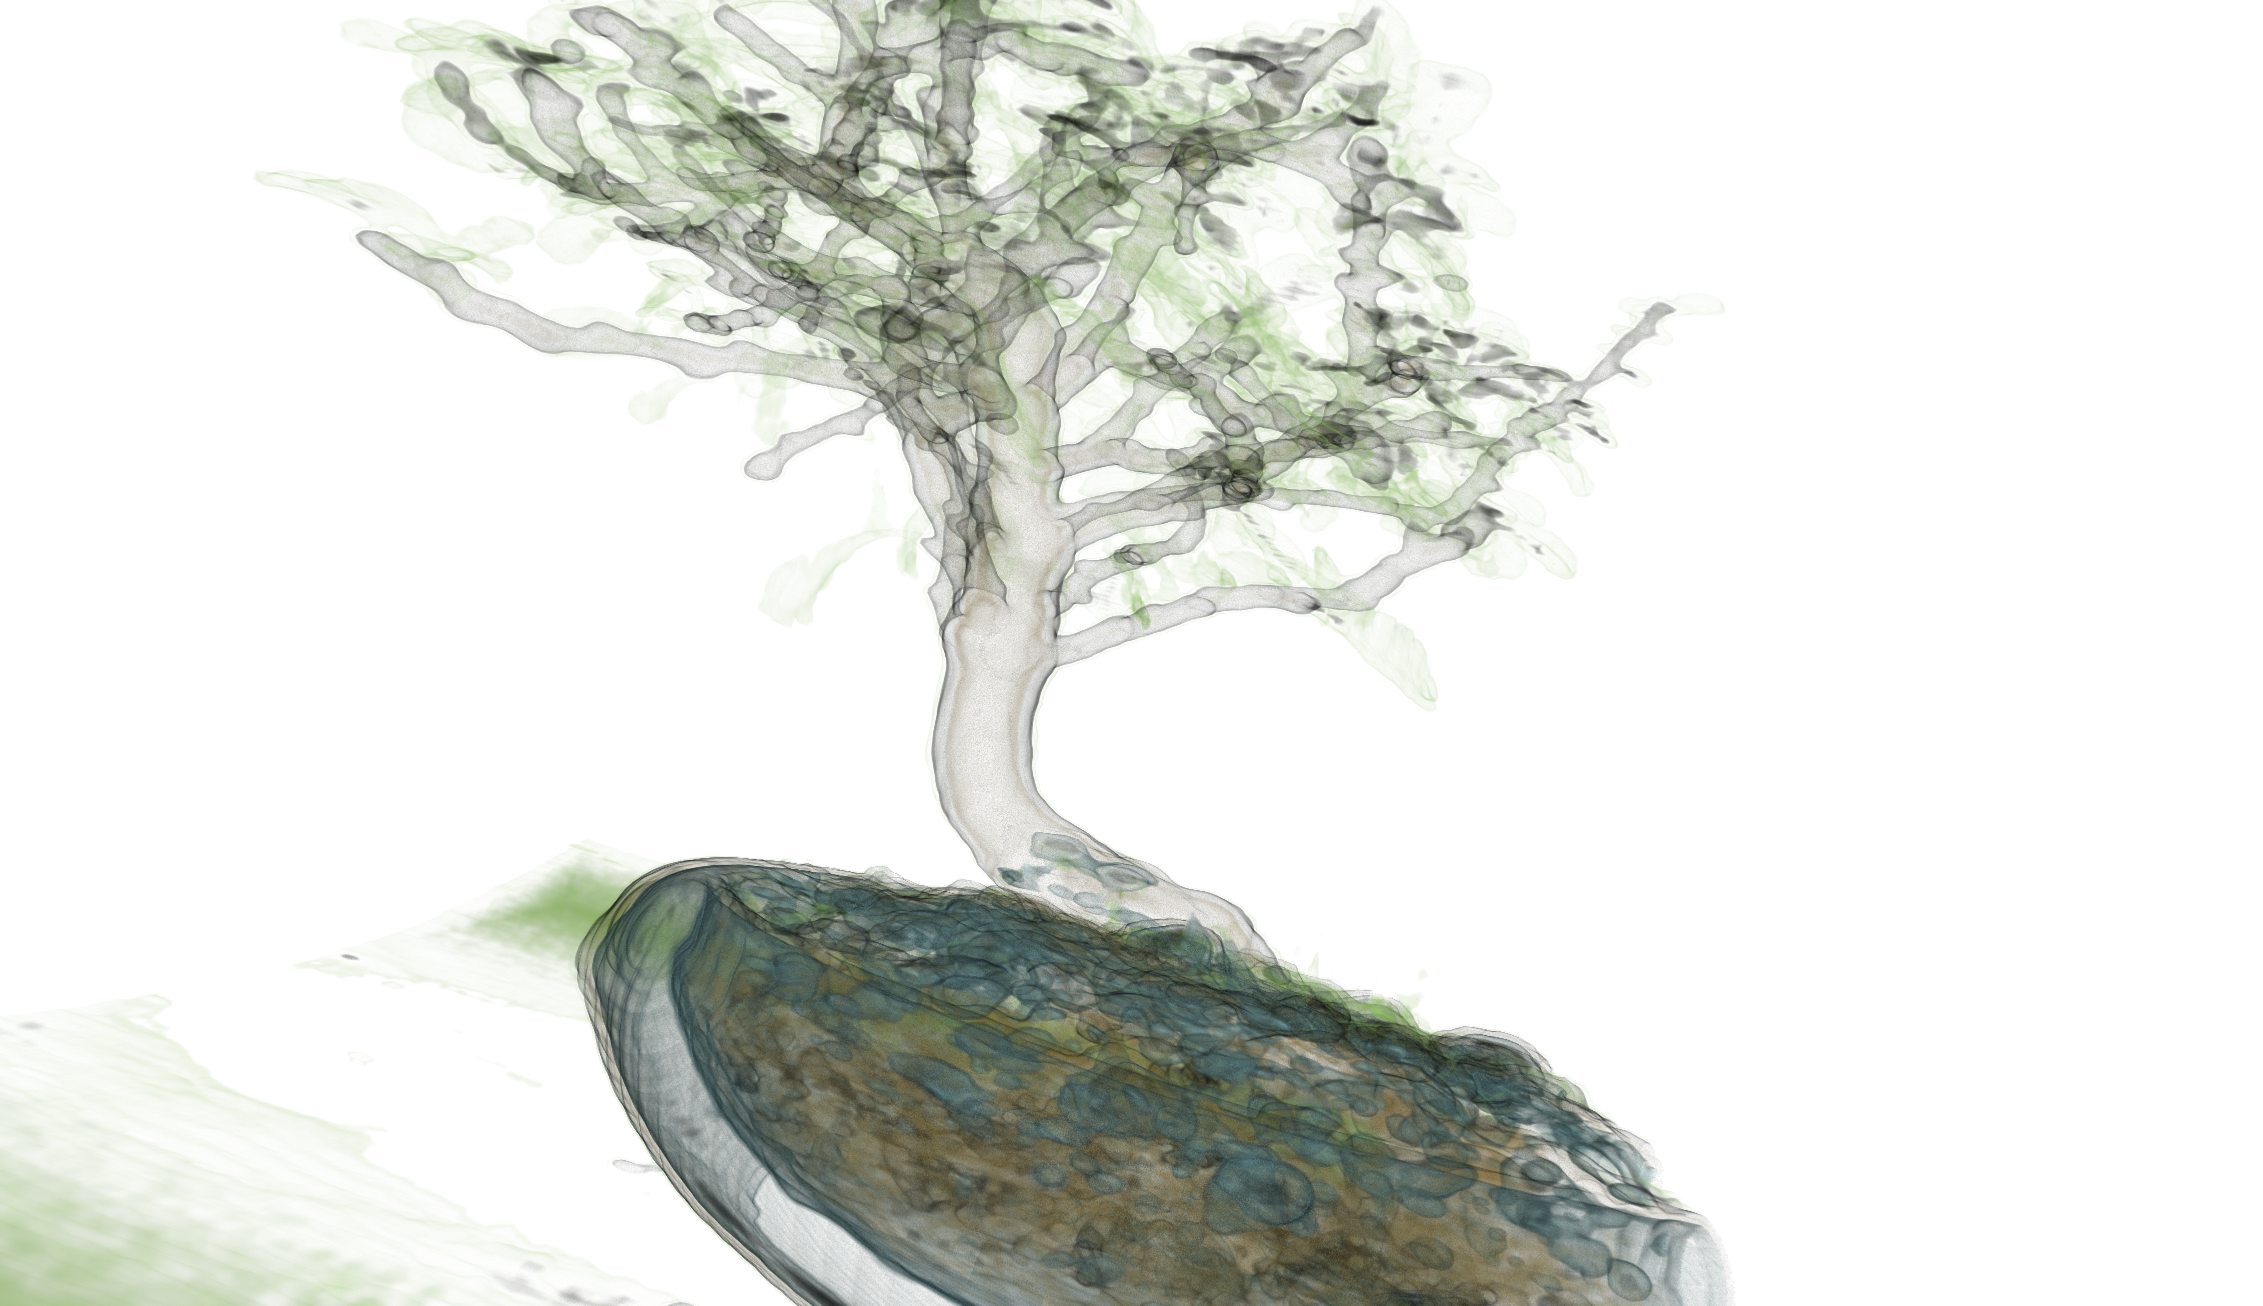
\includegraphics[width=\textheight]{../../Neue_Messungen/Bonsai/st.png}
		\caption{Volumen Bonsai mit ursprünglichem Raycast berechnet. Das Bild hat eine Bildabtastrate von $1$ und eine Strahlabtastrate von $1,5$.}
		\label{fig::res::bon_st}
	\end{figure}
\end{landscape}

\begin{landscape}
	\begin{figure}
		\centering
		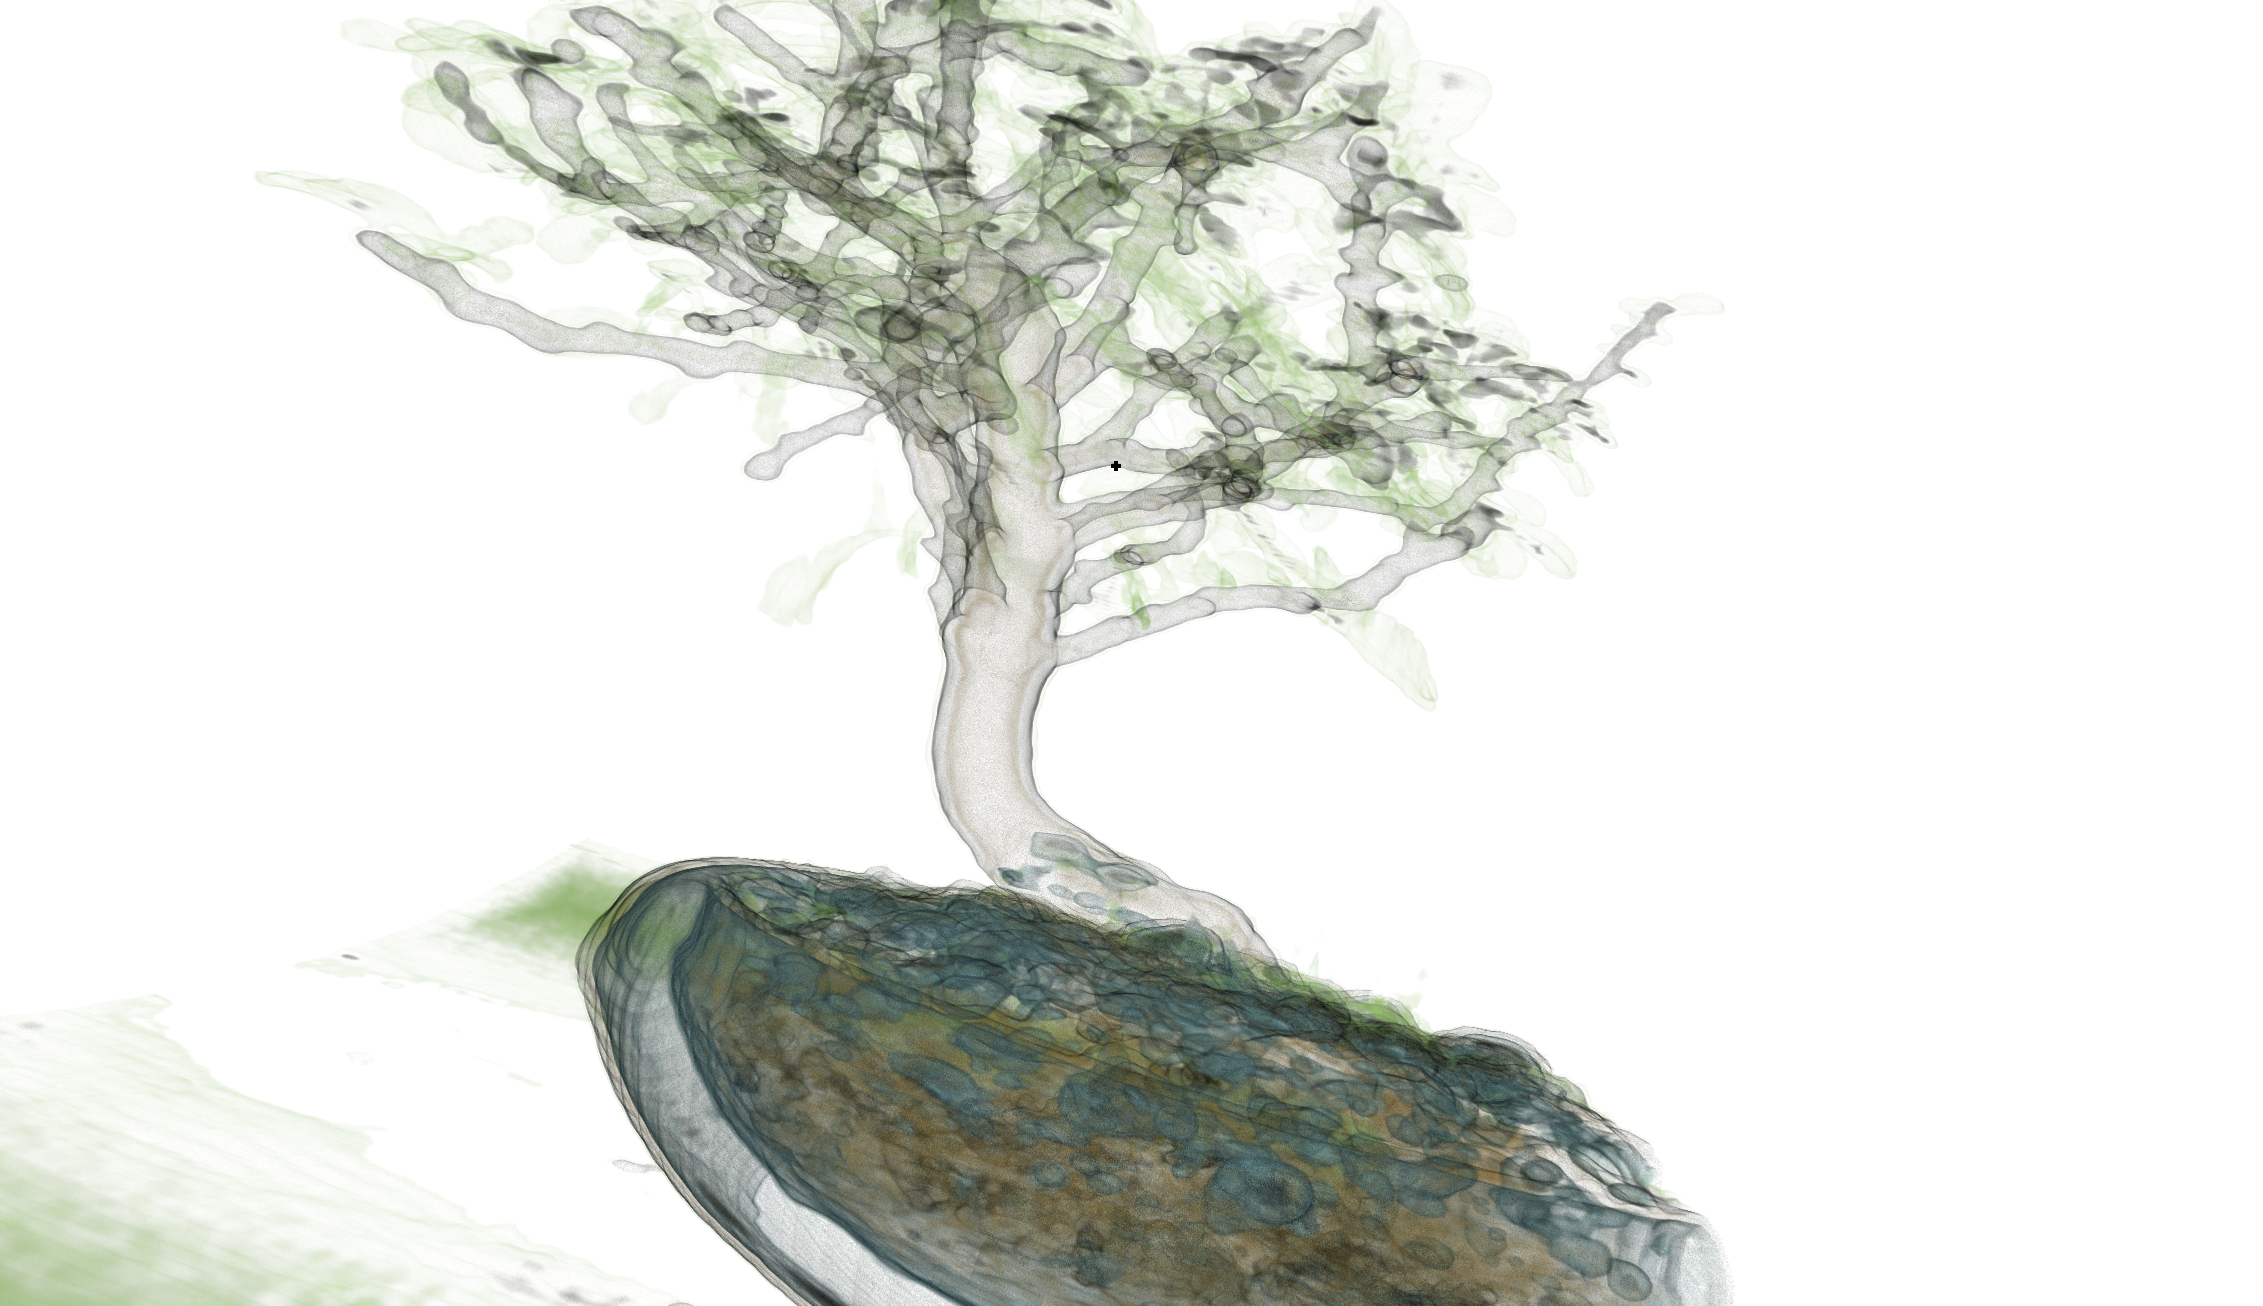
\includegraphics[width=\textheight]{../../Neue_Messungen/Bonsai/st_ors.png}
		\caption{Volumen Bonsai mit modifizierten Standard Raycast berechnet. Die Bildabtastrate beträgt $1$. Die Strahlabtastrate hat an der Mausposition einen Wert von $1,5$ und nimmt, abhängig von der Distanz zur Mausposition, bis zu einem Wert von $\frac{1,5}{4}$ ab.}
		\label{fig::res::bon_st_ors}
	\end{figure}
\end{landscape}

\subsubsection{MDC Raycast}\label{ss::res::mdc}
Der \emph{MDC} Raycast ist das Ergebnis des Arbeitspakets, aus dem Abschnitt \ref{ss::MDC}.
Die Abbildung \ref{fig::res::bon_mdc} zeigt das Volumen \emph{Bonsai}, welches mit dem \emph{MDC} Raycast erstellt wurde.
Das Bild wurde dabei aus der selben Perspektive und mit der gleichen Transferfunktion berechnet, wie dies auch in Abbildung \ref{fig::res::bon_st} der Fall war.

Die maximale Bildabtastrate in Abbildung \ref{fig::res::bon_mdc} hat einen Wert von $0,96$ statt einem Wert von $1,0$.
Damit wird einer leichten Verschiebung des Bildes, aufgrund der zwei unterschiedlichen Bildabtastraten, entgegengewirkt.
Die Anpassung der Bildabtastrate ist abhängig von der Auflösung des Bildes.

In diesem Fall, beim \emph{MDC} Raycast, wurden zwei Bilder berechnet, welche anschließend passend zusammengefügt wurden.
Das erste Bild wurde mit nur einem Viertel der Auflösung berechnet, also der halben Bildabtastrate, und anschließend auf die ursprüngliche Auflösung interpoliert.
Das zweite Bild wurde mit der ursprünglichen Auflösung berechnet, dafür aber nur ein rechteckiger Ausschnitt um die Mausposition.
Anschließend wurde das zweite Bild an der Mausposition in das auf die normale Auflösung interpolierte erste Bild eingefügt.

An den Konturen der Abbildung \ref{fig::res::bon_mdc} ist ein leichter Abfall der Auflösung des Bildes zu erkennen.
Die Konturen, welche in Abbildung \ref{fig::res::bon_st} noch weich gezeichnet wurden, haben außerhalb des Rechtecks um die Mausposition nun Artefakte der Unterabtastung, wie zum Beispiel leichte Treppenstufen.
Innerhalb des Rechtecks sind die Konturen immer noch weich gezeichnet und es ist dort kein Unterschied zu Abbildung \ref{fig::res::bon_st} zu sehen.

Die Größe des Rechtecks beträgt $350$\,Pixel in x- und y-Richtung und ist groß genug, dass die Abnahme der Auflösung im äußeren Bereich, bei Fokussierung der Mausposition, nicht wahrnehmbar ist.
Wird bei aktivem Eyetracking anstelle der Mausposition die Blickposition verwendet, so ist der aktuell betrachtete Bereich immer hoch aufgelöst.
Ein Unterschied zwischen den beiden Bereichen fällt während einer Fokussierung kaum auf.
Wenn der Fokus langsam über das Bild wandert, kann man einen Unterschied zwischen den Auflösungen erkennen.
An dem Übergang des normal aufgelösten Bereichs zu dem Bereich mit der halben Auflösung kommt es während einer Bewegung an den Konturen des Volumen zu leichten Veränderungen.
Diese können die Aufmerksamkeit auf sich ziehen und daher auffallen.

Obwohl der Bereich außerhalb des Rechtecks mit nur einem Viertel der Auflösung innerhalb des Rechtecks berechnet wurde, ist die Bildqualität in diesem Bereich noch recht gut.
Da die Sehschärfe mit zunehmenden Winkel von der Fovea weg immer weiter abnimmt, könnte die Bildabtastrate außerhalb des Rechtecks vermutlich weiter gesenkt werden, ohne dass dies die Bildqualität bei der Verwendung eines Eyetrackers beeinträchtigt.

Abbildung \ref{fig::res::bon_mdc_ors} zeigt die selbe Berechnung wie Abbildung \ref{fig::res::bon_mdc} aber mit einer variierten Strahlabtastrate.
Anders als in Abbildung \ref{fig::res::bon_st_ors}, in welcher ebenfalls die Strahlabtastrate auf die gleiche Weise über das Bild hinweg variiert wurde, macht sich in Abbildung \ref{fig::res::bon_mdc_ors} an zum Beispiel den Ästen, die geringere Strahlabtastrate bemerkbar.
Die Flächen der Äste erscheinen ein bisschen löchrig, da Voxel teilweise übersprungen werden.
Wird die Mausposition fokussiert, kann man dies, aufgrund der Distanz zum Blickpunkt, nicht wahrnehmen.

\begin{landscape}
	\begin{figure}
		\centering
		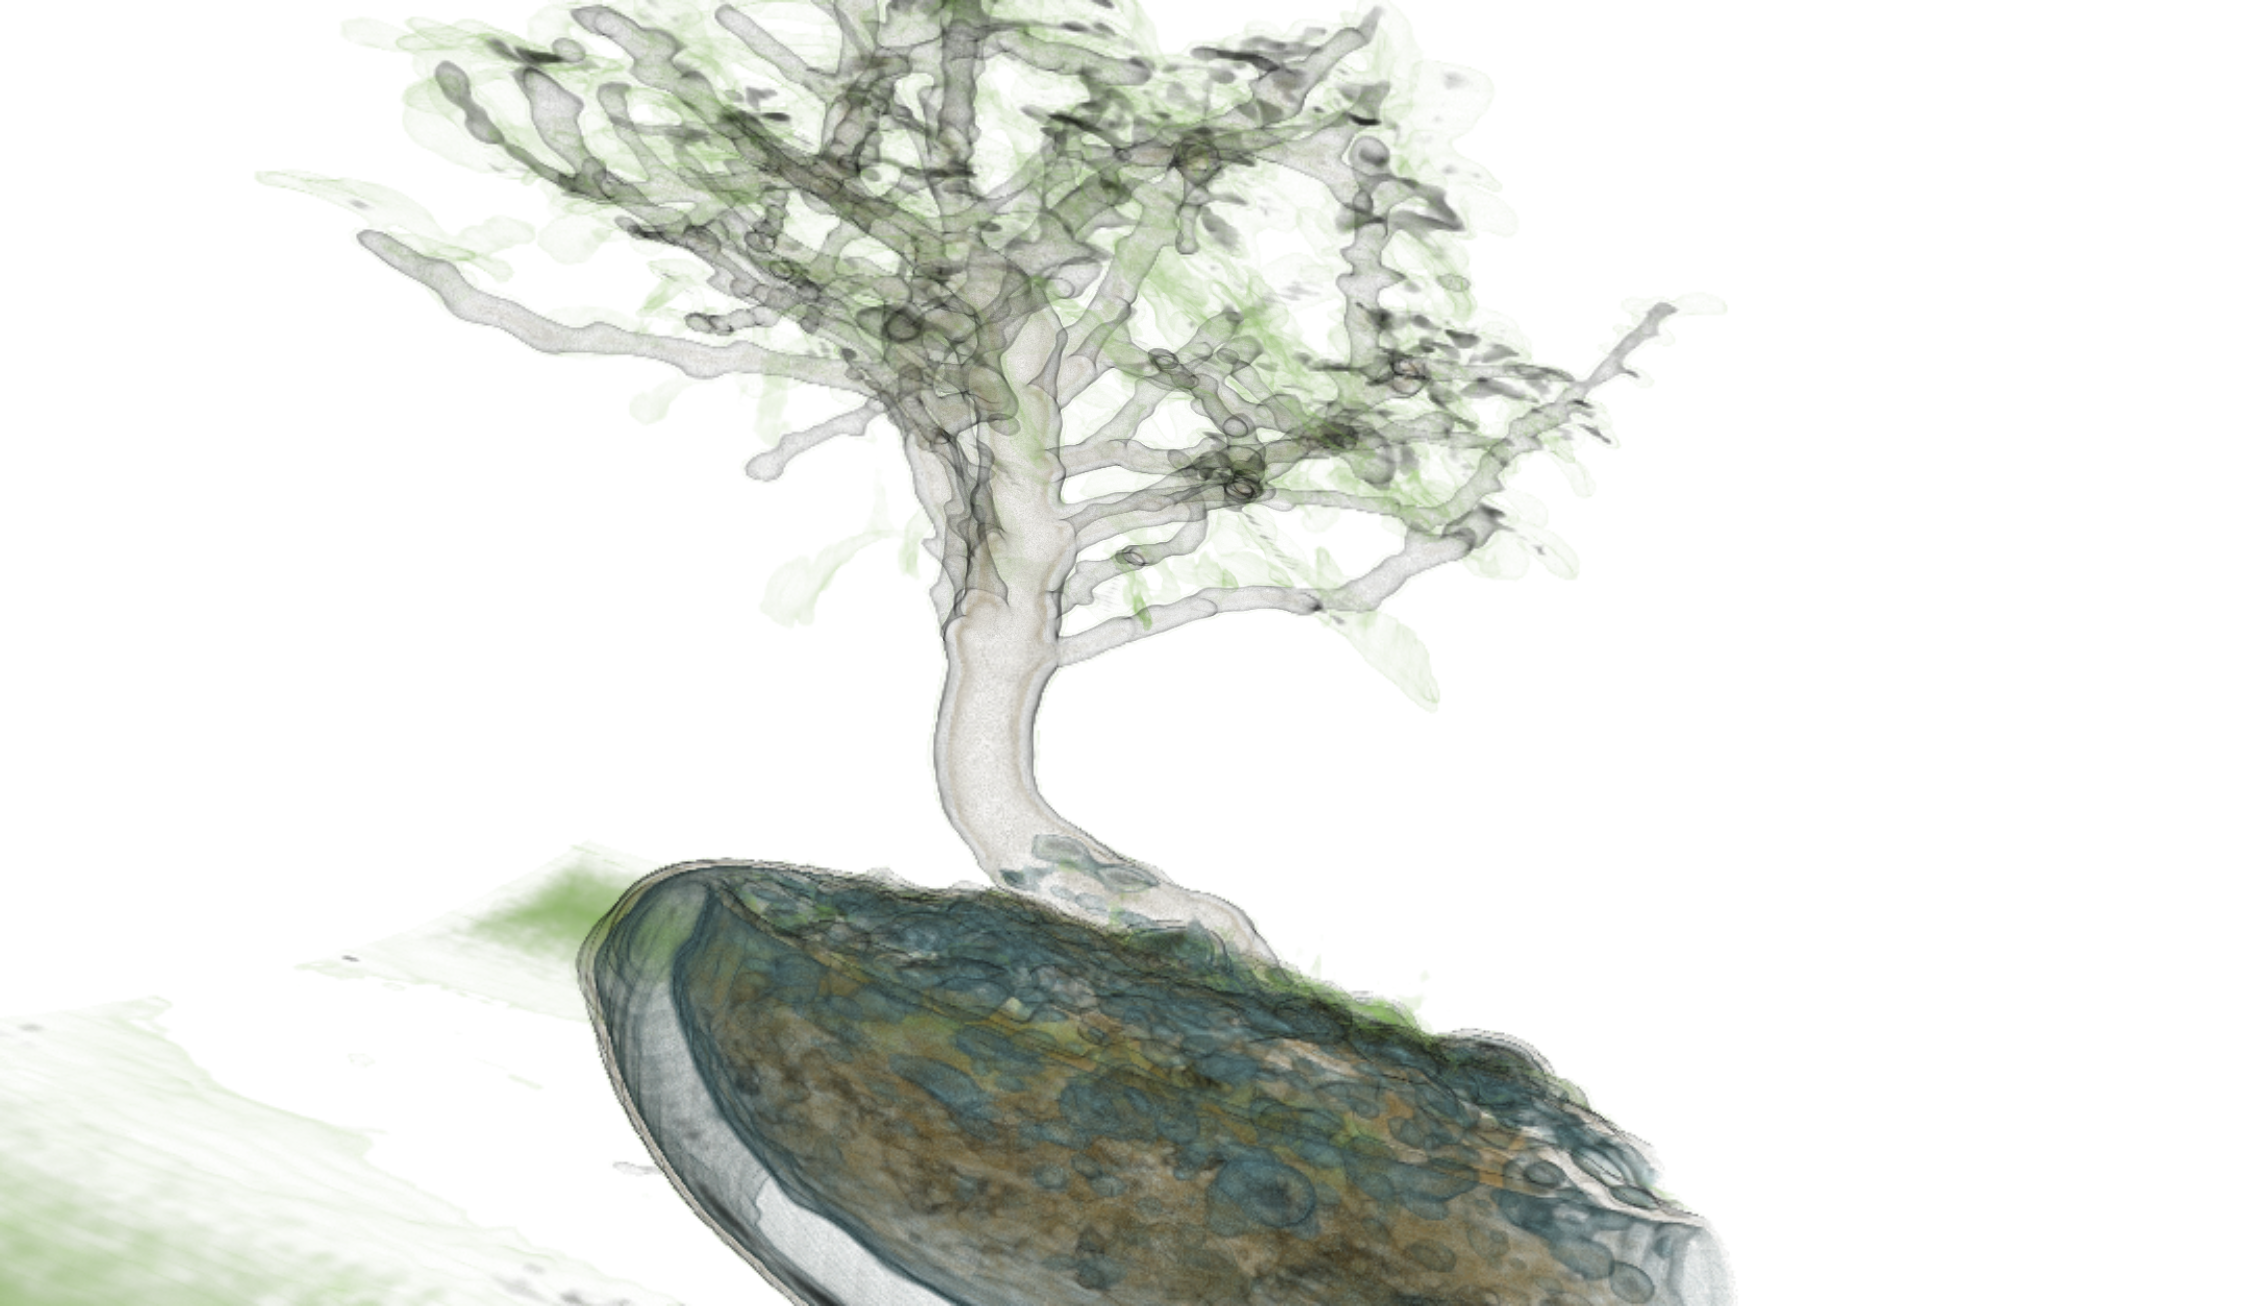
\includegraphics[width=1\textheight]{../../Neue_Messungen/Bonsai/mdc.png}
		\caption{Volumen Bonsai. Das Bild wurde mit dem \emph{MDC} Raycast berechnet. Ein kleiner Teil des Bildes, in Form eines Rechtecks, hat eine Bildabtastrate von $1,0$. Das restliche Bild hat nur eine Bildabtastrate von $0,5$. Die Strahlabtastrate beträgt für das ganze Bild $1.5$.}
		\label{fig::res::bon_mdc}
	\end{figure}
\end{landscape}

\begin{landscape}
	\begin{figure}
		\centering
		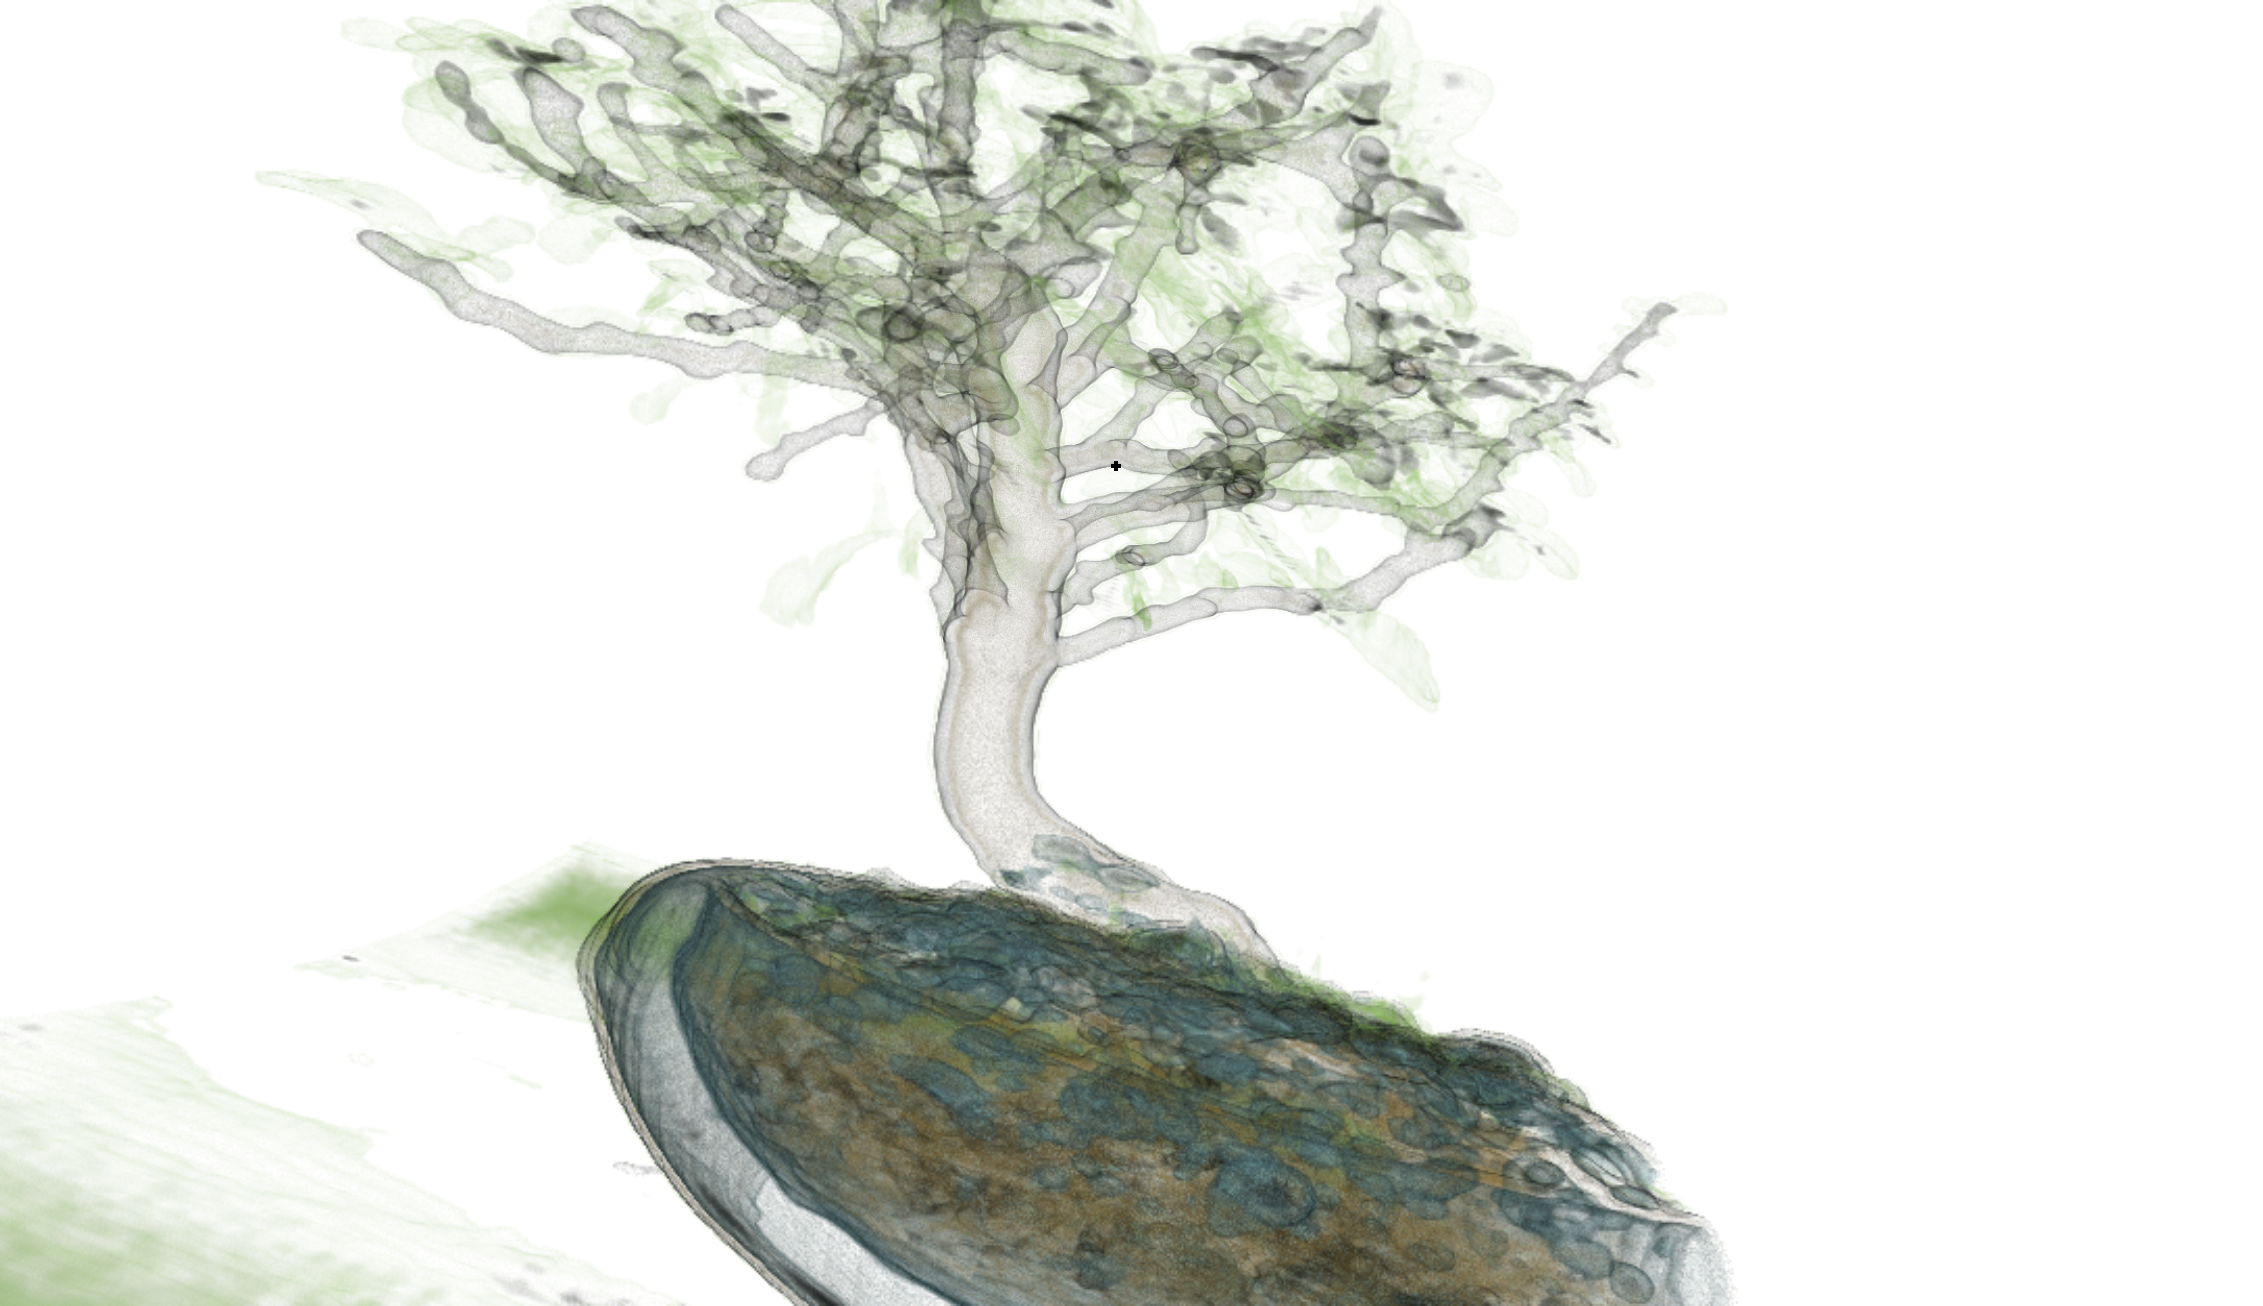
\includegraphics[width=1\textheight]{../../Neue_Messungen/Bonsai/mdc_ors.png}
		\caption{Volumen Bonsai. Das Bild wurde mit dem \emph{MDC} Raycast berechnet. Ein kleiner Teil des Bildes, in Form eines Rechtecks, hat eine Bildabtastrate von $1,0$. Das restliche Bild hat nur eine Bildabtastrate von $0,5$. Die Strahlabtastrate hat an der Mausposition einen Wert von $1,5$ und nimmt, abhängig von der Distanz zur Mausposition, bis zu einem Wert von $\frac{1,5}{4}$ ab.}
		\label{fig::res::bon_mdc_ors}
	\end{figure}
\end{landscape}

\subsubsection{DDC Raycast}\label{ss::res::ddc}
Der \emph{DDC} Raycast ist das Ergebnis des Arbeitspakets aus dem Abschnitt \ref{ss::DDC}.
Abbildung \ref{fig::res::bon_ddc} zeigt das Volumen \emph{Bonsai}, welches mit dem \emph{DDC} Raycast erstellt wurde.
Das Bild wurde aus der selben Perspektive und mit der gleichen Transferfunktion berechnet, wie in den Abbildungen \ref{fig::res::bon_st} und \ref{fig::res::bon_mdc}.
Die maximale Bildabtastrate ist $1$.
Diese nimmt in zwei Stufen nach außen hin ab.

Beim \emph{DDC} Raycast wurde nur ein Aufruf des Raycasts gestartet und die Work-Items und ihre entsprechenden Strahlen auf verschiedene Bildpunkte abgebildet.
Das gesamte Bild wurde in einem zweiten Kernel Aufruf interpoliert.
Innerhalb eines kleinen Bereichs in der Form einer Ellipse um den Blickpunkt herum hat das Bild eine Bildabtastrate von $1$, dass heißt jeder Pixel entspricht einem Farbwert der Auswertung eines Strahls.
Außerhalb von diesem Bereich aber innerhalb einer zweiten größeren und umschließenden Ellipse hat das Bild in x- und y-Richtung eine Bildabtastrate von $\frac{1}{2}$.
Das heißt, dass in x- und y-Richtung nur für jedes zweiten Pixel ein Strahl ausgewertet wird.
In dem äußersten Bereich beträgt die Bildabtastrate in x- und y-Richtung $\frac{1}{7}$.
Es wird also in jedem $7\times7$\,Pixel-Feld nur ein Strahl ausgewertet.
Die die Farbwerte der Pixel, die selbst nicht durch einen Strahl bestimmt wurden, wurden durch vier umliegende Farbwerte von Strahlen bilinear interpoliert.

In Abbildung \ref{fig::res::bon_ddc} ist deutlich zu sehen, dass der Großteil des Bildes eine geringe Auflösung hat.
In dem am niedrigsten abgetasteten Bereich sind an den Konturen, insbesondere die der Äste, deutliche Merkmale der Unterabtastung zu sehen.
In Abbildung \ref{fig::res::bon_st} und \ref{fig::res::bon_mdc} verlaufen die Konturen der Äste noch diagonal und sind relativ weich gezeichnet, hier haben sie starke Treppeneffekte.
Manche Konturen sind auch teilweise unterbrochen.

In dem mittleren Bereich ist die Bildqualität recht gut und das Bild scharf zu erkennen.
Trotzdem hat das Bild hier nur ein Viertel der Auflösung.
Den Übergang zwischen dem mittleren und inneren Bereich, welcher die normale Auflösung hat, ist kaum zu erkennen.
Aufgrund des starken Abfalls der Bildabtastrate vom mittleren zum äußeren Bereich, fällt dieser Übergang stärker auf.

Bei aktivem Eyetracking wird anstelle der Mausposition die aktuelle Blickposition verwendet.
Der Fokus liegt bei aktivem Eyetracking nun im Zentrum des inneren Bereichs, dieser wurde hier mit der Mausposition simuliert und ist als schwarzes Kreuz eingezeichnet.
Der innere Bereich ist groß genug, so dass der Abfall der Bildabtastrate zum mittleren Bereich nicht auffällt.
Zusammen ergeben der innere und mittlere Bereich den Teil des Bildes, in welchem das Bild scharf zu sehen ist.
Dieser ist ausreichend groß, dass der Bereich an und um dem Blickpunkt immer scharf wahrgenommen wird.
Anders als in Abbildung \ref{fig::res::bon_mdc}, ist es in Abbildung \ref{fig::res::bon_ddc} auch wenn der innere und mittlere Bereich auf den Blickpunkt zentriert sind, auffallend, dass der äußere Bereich mit einer deutlich niedrigeren Bildabtastrate berechnet wurde.
Die grundlegenden Konturen des Bildes können aber im äußeren Bereich noch erkannt werden wodurch das Identifizieren von interessanten Objekten immer noch möglich ist.

Abbildung \ref{fig::res::bon_ddc_ors} zeigt die selbe Berechnung wie Abbildung \ref{fig::res::bon_ddc} aber mit einer variierten Strahlabtastrate, wie sie in Abbildung \ref{fig::res::bon_st_ors} und \ref{fig::res::bon_mdc_ors} auch der Fall war.
Wie in Abbildung \ref{fig::res::bon_mdc_ors} erscheinen Teile, der von der Mausposition weiter entfernten Objekte, löchrig.
Der Unterschied zwischen variierter und nicht-variierter Strahlabtastrate fällt bei der DDC Raycast Methode ein wenig stärker auf, als bei der MDC Raycast Methode.
Trotzdem ist beeinflusst die viel niedrigere Auflösung im äußeren Bereich die Bildqualität viel maßgebender, als die reduziert Strahlabtastrate, so dass diese kaum mehr die Wahrnehmung beeinträchtigt.
Dies ist noch weniger der Fall, wenn die Mausposition fokussiert wird.

\begin{landscape}
	\begin{figure}
		\centering
		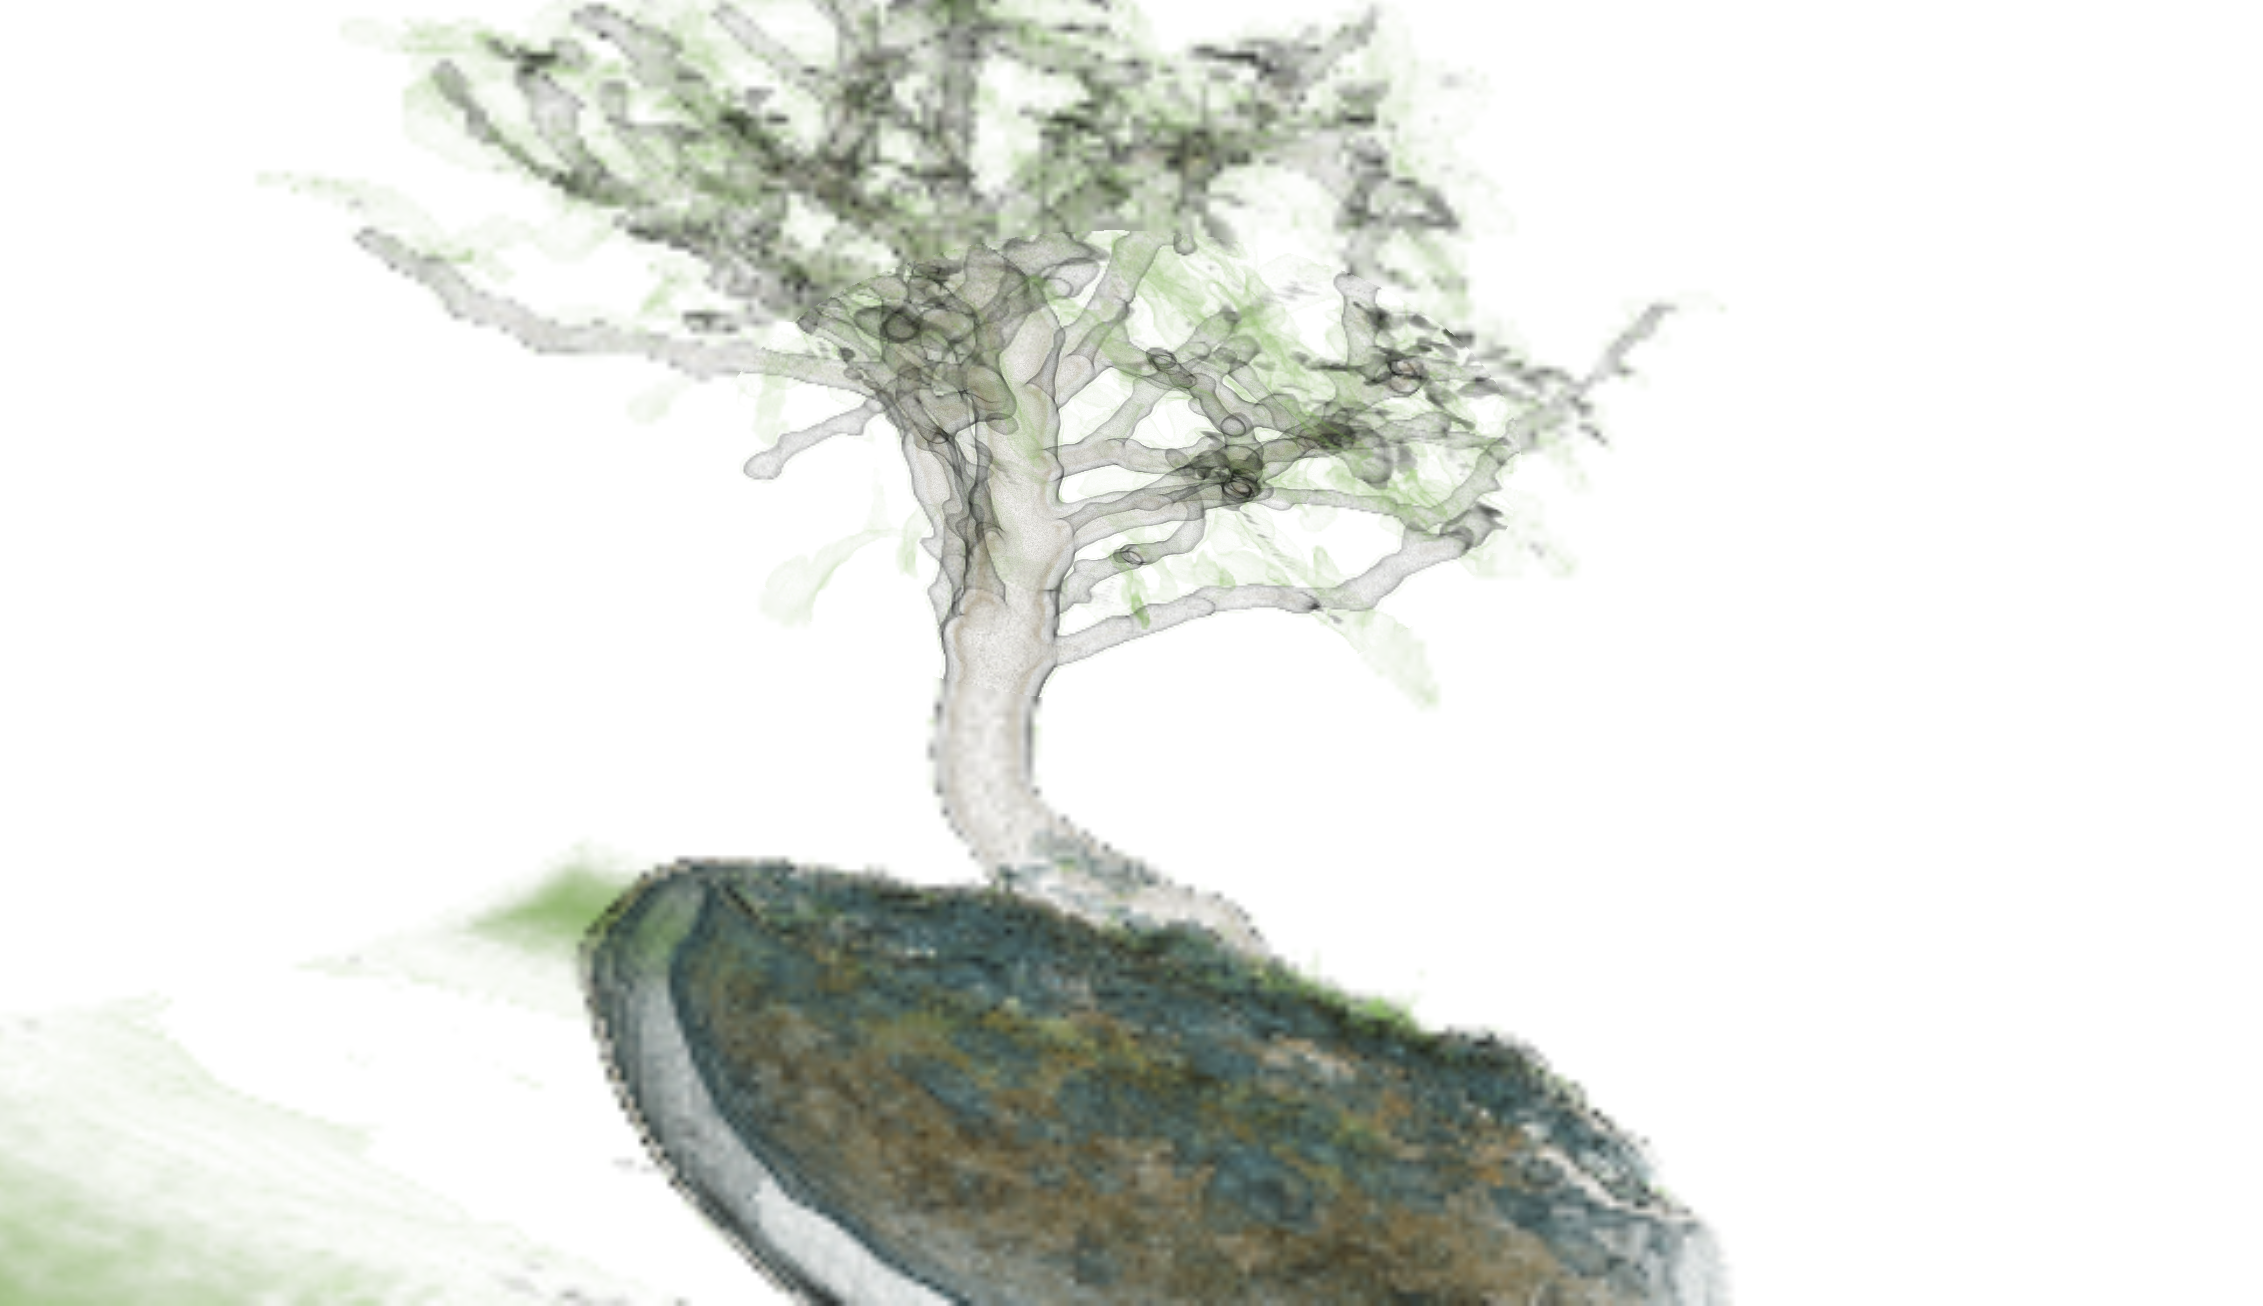
\includegraphics[width=1\textheight]{../../Neue_Messungen/Bonsai/ddc.png}
		\caption{Volumen Bonsai mit \emph{DDC} Raycast berechnet. Die Bildabtastrate nimmt nach außen hin in zwei Schritten ab. An der Mausposition hat sie den höchsten Wert von $1,0$. Etwas weiter außen einen Wert von $0,5$ und noch weiter außen hat sie den niedrigsten Wert von $\frac{1}{7}$. Die Strahlabtastrate beträgt für das ganze Bild $1.5$.}
		\label{fig::res::bon_ddc}
	\end{figure}
\end{landscape}

\begin{landscape}
	\begin{figure}
		\centering
		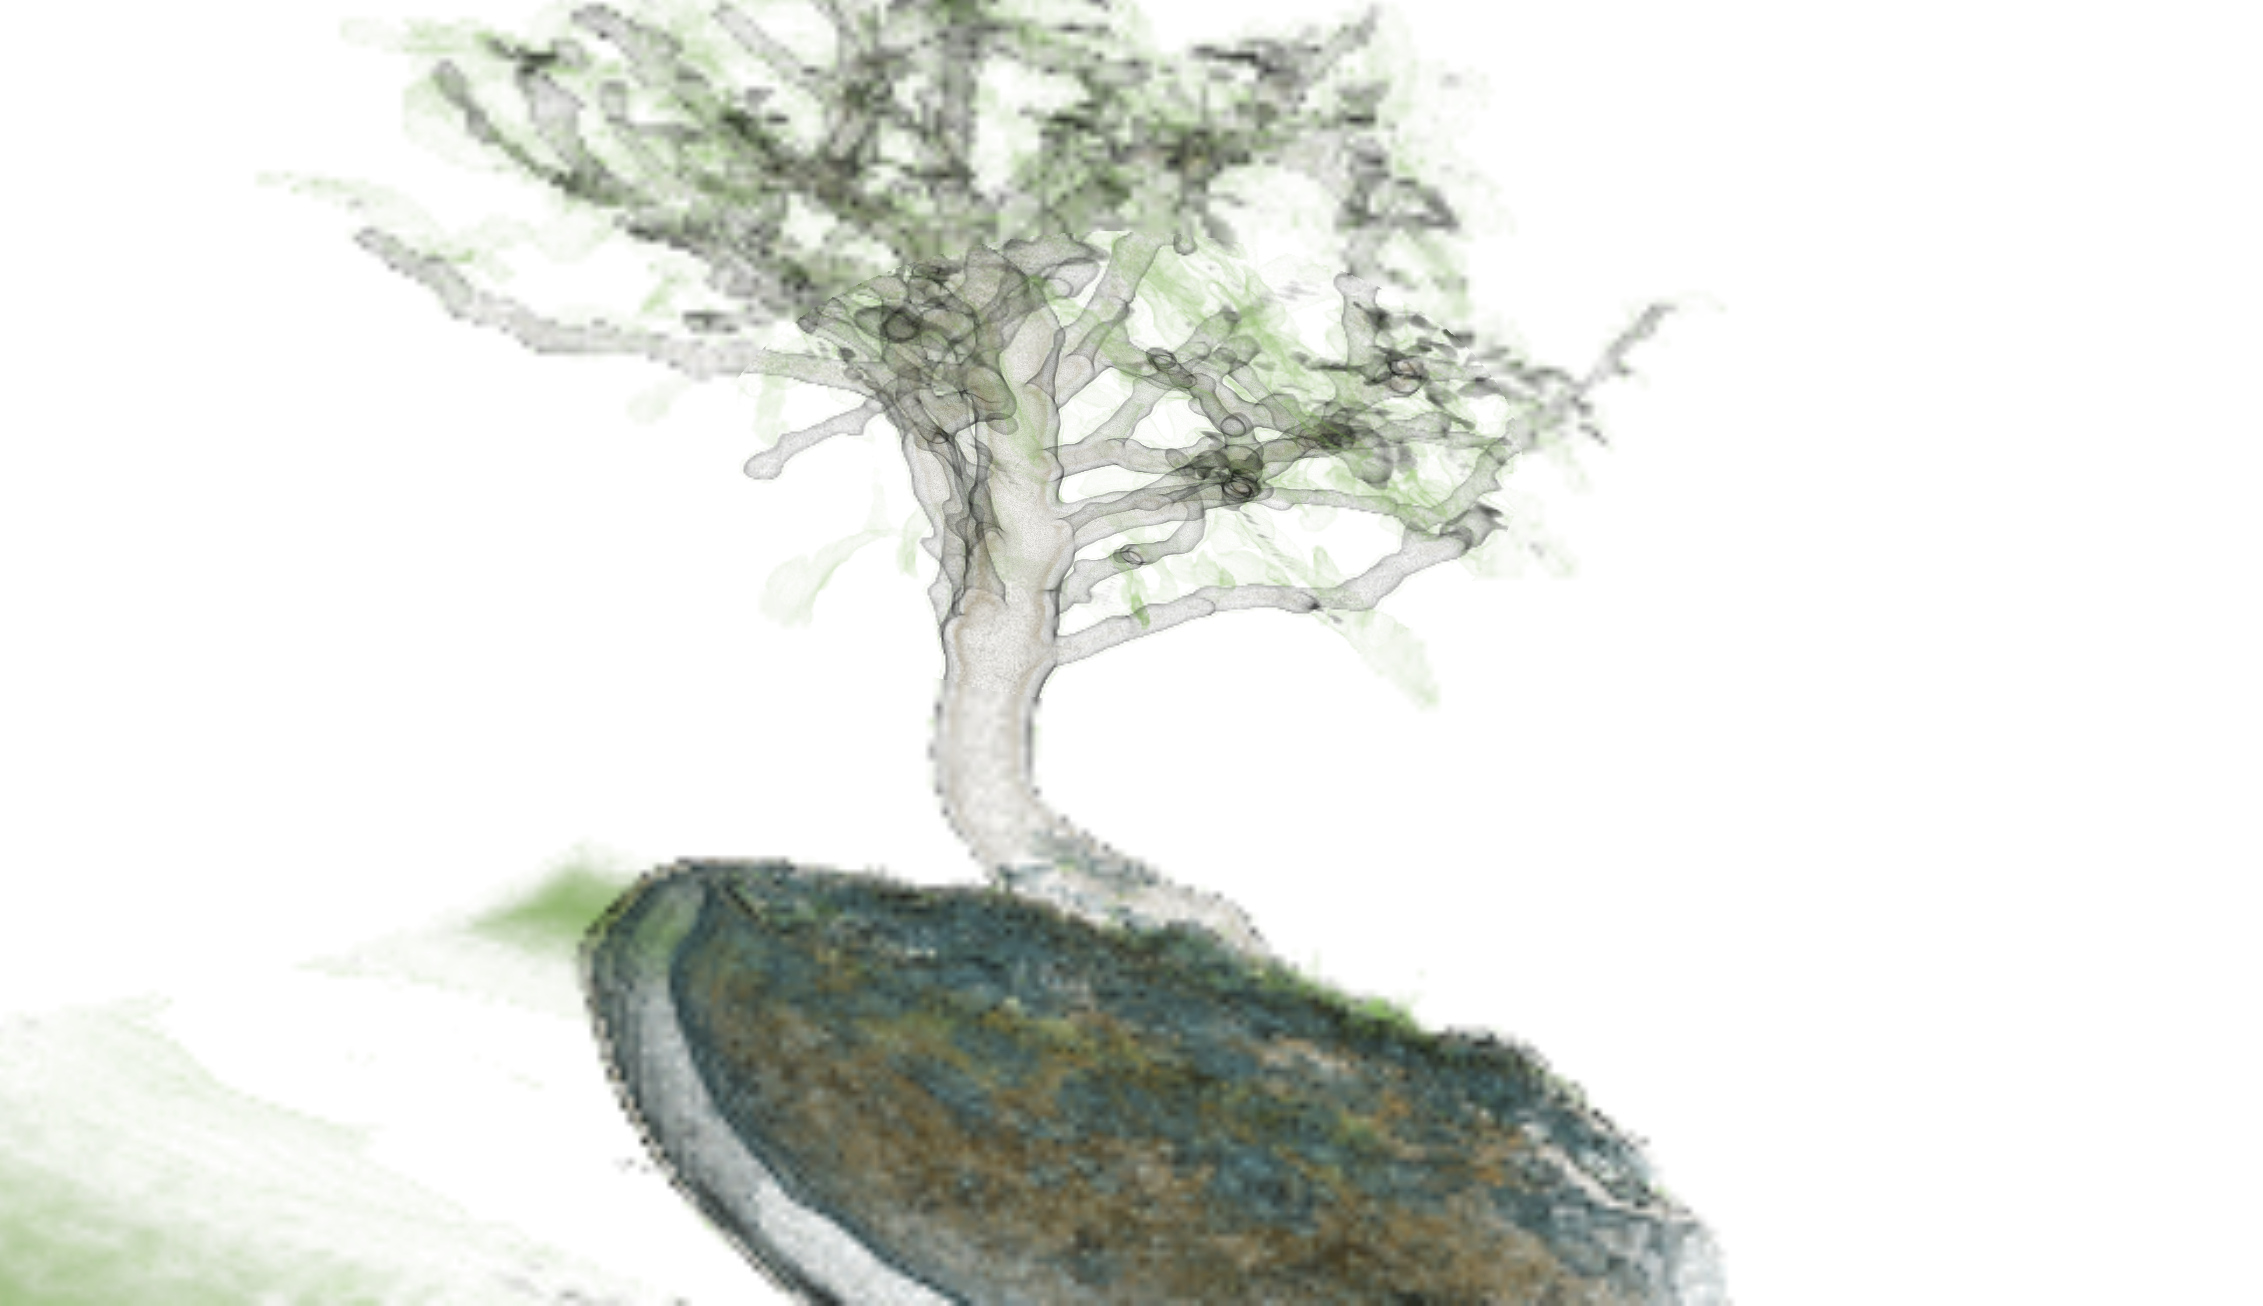
\includegraphics[width=1\textheight]{../../Neue_Messungen/Bonsai/ddc_ors.png}
		\caption{Volumen Bonsai mit \emph{DDC} Raycast berechnet. Die Bildabtastrate nimmt nach außen hin in zwei Schritten ab. An der Mausposition hat sie den höchsten Wert von $1,0$, weiter außen einen Wert von $0,5$, dann einen Wert von $\frac{1}{7}$. Die Strahlabtastrate hat an der Mausposition einen Wert von $1,5$ und nimmt, abhängig von der Distanz zur Mausposition, bis zu einem Wert von $\frac{1,5}{4}$ ab.}
		\label{fig::res::bon_ddc_ors}
	\end{figure}
\end{landscape}

\subsubsection*{Direkter Vergleich}
Abbildung \ref{fig::res::sn_comp_st_123} zeigt eine Berechnung des zweiten Volumens, welche mit dem Standard Raycast und ohne einer variierten Strahlabtastrate berechnet wurde.
Anders als das erste Volumen, welches ein ct-scan ist, ist dieses der $1353$-te Zeitschritt aus der Simulation einer \emph{shock wave formation in core-collapse supernova} von John Blondin, NCSU.
Es hat eine Auflösung von $432\times432\times432$\,Voxel, welche ebenfalls in x-, y- und z-Richtung eine Skalierung von $1,0$ haben.
Die Dichte der Voxel gibt die physikalische Entropie an der Position in der Simulation an.

In Abbildung \ref{fig::res::sn_comp_st_123} sind drei Kästchen eingezeichnet und nummeriert.
Für jede der Berechnungsmethoden wurde das Volumen mit der gleichen Transferfunktion und Perspektive beziehungsweise Kameraausrichtung berechnet.
Für jede der Berechnungen sind die drei Ausschnitte vergrößert worden und nebeneinander der Reihe nach aufgeführt.
Die Mausposition für die jeweiligen Berechnungen war dabei immer an der selben Position und ist jeweils in Ausschnitt $2$ eingezeichnet.

Ausschnitt $1$ liegt etwas weiter weg von der Mausposition aber circa am Übergang des mittleren Bereichs zum äußeren Bereich des \emph{DDC} Raycasts.
Die Strahlabtastrate wäre entsprechend in Ausschnitt $1$ ein wenig geringer, als an der Mausposition, falls eine Methode mit variierte Strahlabtastrate verwendet wurde.
Ausschnitt $2$ enthält die Mausposition und ist dementsprechend jeweils im inneren Bereich mit einer Bildabtastrate von $1$.
Die Strahlabtastrate ist hier ebenfalls fast maximal bei $1,5$.
Ausschnitt $3$ liegt relativ zur Auflösung des Bildes weit von der Mausposition entfernt.
Die Bildabtastrate beträgt hier für den Standard Raycast $1$, für den \emph{MDC} Raycast $\frac{1}{2}$ und für den \emph{DDC} Raycast $\frac{1}{7}$.
Wird eine Methode mit variierte Strahlabtastrate verwendet, so hat diese in Ausschnitt $3$ fast den minimalen Wert von $\frac{1,5}{4}$.

Da die Mausposition sich innerhalb des zweiten Ausschnitts befindet, ist die Strahlabtastrate und die Bildabtastrate hier immer fast maximal, so dass Ausschnitt $2$ in den verschiedenen Methoden fast identisch ist.
Auch ist hier auffallend, dass obwohl, dass die Strahlabtastrate in Ausschnitt $3$ bei der Verwendung des selben Raycast mit einmal konstanter Strahlabtastrate und variierter Strahlabtastrate, sehr unterschiedlich ist, dies sich bei diesem Bild aber kaum auswirkt und nicht wahrgenommen wird.
Womöglich liegt das daran, dass durch die Transferfunktion in diesem Volumen eher größere und dickere Strukturen hervorgehoben wurden und daher selbst bei einer deutlich geringeren Strahlabtastrate diese Strukturen genügend oft abgetastet wurden.

Die eigentlichen Unterschiede sieht man bei der Verwendung verschiedener Raycasts besonders in Ausschnitt $1$.
So ist mit dem Standard Raycast der gesamte Ausschnitt $1$ scharf zu sehen (siehe Abbildung \ref{fig::res::sn_comp_st_ors}), während bei dem \emph{MDC} Raycast an den Konturen am Rand des Volumens zu sehen ist, dass diese leicht unschärfer sind (siehe Abbildung \ref{fig::res::sn_comp_mdc_ors}).
Ausschnitt $3$ unterscheidet sich hier zwischen dem Standard Raycast und dem \emph{MDC} Raycast kaum.

Ein wesentlicher Unterschied ist sowohl in Ausschnitt $1$ als auch in Ausschnitt $3$ zwischen dem \emph{DDC} Raycast und dem \emph{MDC} sowie dem Standard Raycast wahrnehmbar.
Man kann sehen, dass der äußere Bereich des \emph{DDC} Raycast (siehe Abbildung \ref{fig::res::sn_comp_ddc_ors}), deutlich unschärfer ist, als der äußere Bereich des \emph{MDC} Raycast (siehe Abbildung \ref{fig::res::sn_comp_mdc_ors}).

\begin{figure}
	\centering
	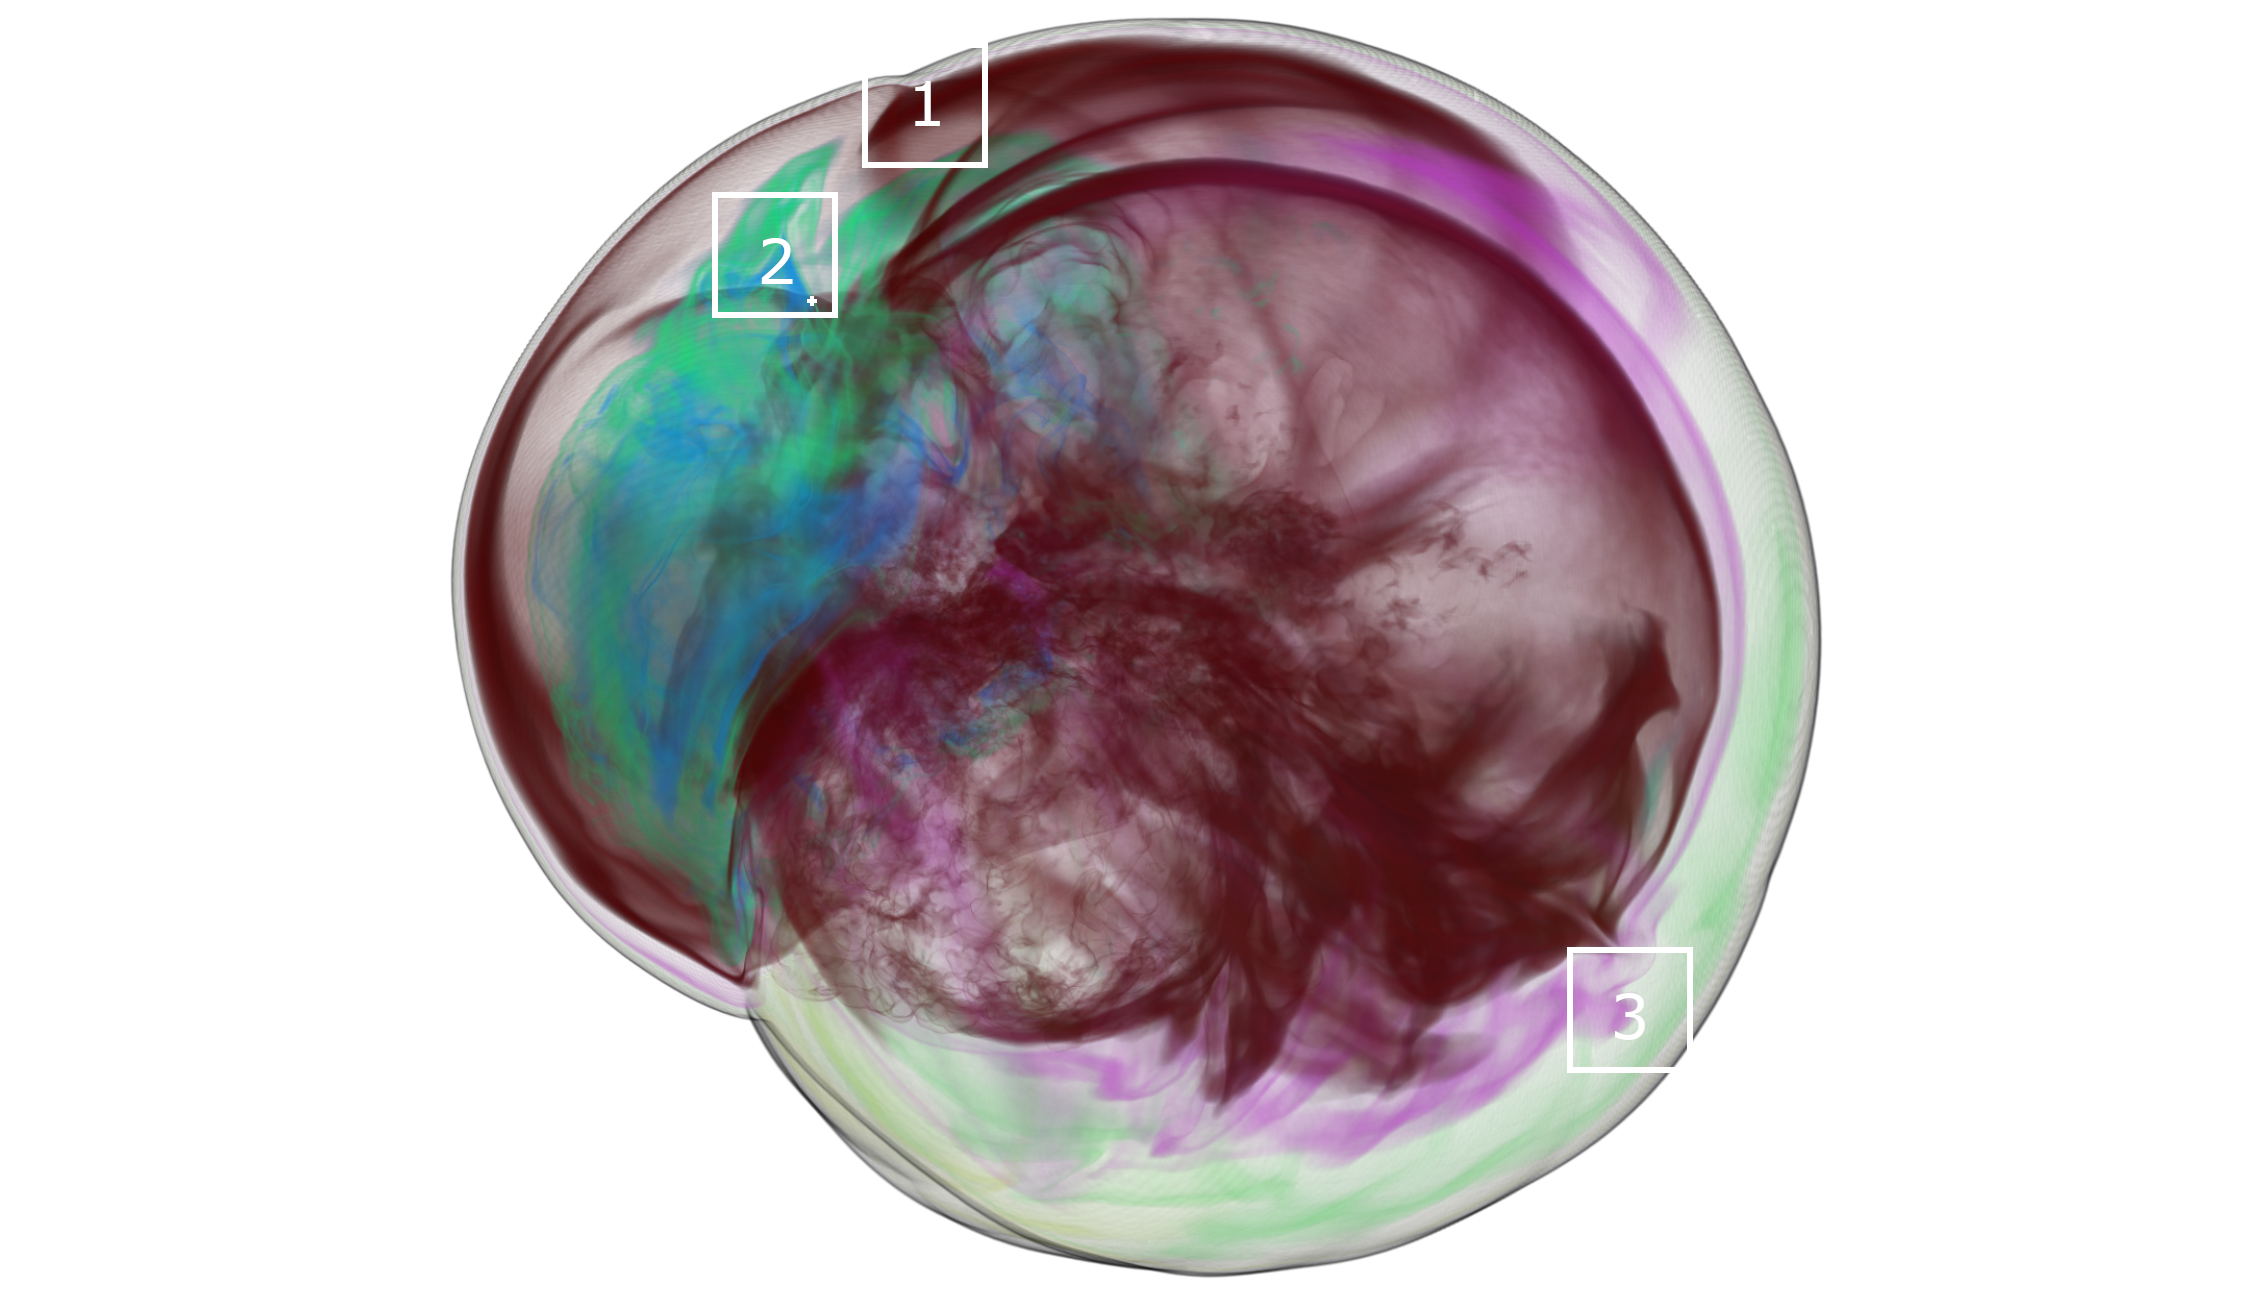
\includegraphics[width=0.7\textwidth]{../../Neue_Messungen/Supernova/cut/st/st_123.png}
	\caption{Ein Zeitschritt der Supernova mit dem Standard Raycast berechnet. Die Bildabtastrate beträgt für das ganze Bild $1$. Die Strahlabtastrate beträgt für das ganze Bild $1,5$. die Mausposition und drei nummerierte Quadrate sind eingezeichnet, die Positionen der Quadrate werden im folgenden Vergleich verwendet.}
	\label{fig::res::sn_comp_st_123}
\end{figure}

\begin{figure}[]
	\centering
	\begin{minipage}[t]{0.3\textwidth}
		\centering
		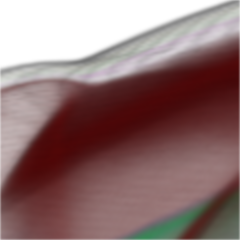
\includegraphics[width=1\textwidth]{../../Neue_Messungen/Supernova/cut/st/st_1.png}
		% \caption*{Quadrat 1 vergrößert dargestellt.}
		% \label{fig::res::sn_comp_st_1}
	\end{minipage}
	\hfill
	\begin{minipage}[t]{0.3\textwidth}
		\centering
		
\includegraphics[width=1\textwidth]{../../Neue_Messungen/Supernova/cut/st/st_2.png}
		% \caption*{Quadrat 2 vergrößert dargestellt.}
		% \label{fig::res::sn_comp_st_2}
	\end{minipage}
	\hfill
	\begin{minipage}[t]{0.3\textwidth}
		\centering
		
\includegraphics[width=1\textwidth]{../../Neue_Messungen/Supernova/cut/st/st_3.png}
		% \caption*{Quadrat 3 vergrößert dargestellt.}
		% \label{fig::res::sn_comp_st_3}
	\end{minipage}
	\caption{Supernova mit Standard Raycast und ohne variierter Strahlabtastrate berechnet.}
	\label{fig::res::sn_comp_st}
\end{figure}

\begin{figure}[]
	\centering
	\begin{minipage}[t]{0.3\textwidth}
		\centering
		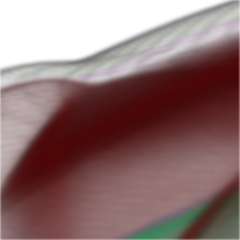
\includegraphics[width=1\textwidth]{../../Neue_Messungen/Supernova/cut/st_ors/st_ors_1.png}
		% \caption*{Quadrat 1 vergrößert dargestellt.}
		% \label{fig::res::sn_comp_st_ors_1}
	\end{minipage}
	\hfill
	\begin{minipage}[t]{0.3\textwidth}
		\centering
		
\includegraphics[width=1\textwidth]{../../Neue_Messungen/Supernova/cut/st_ors/st_ors_2.png}
		% \caption*{Quadrat 2 vergrößert dargestellt.}
		% \label{fig::res::sn_comp_st_ors_2}
	\end{minipage}
	\hfill
	\begin{minipage}[t]{0.3\textwidth}
		\centering
		
\includegraphics[width=1\textwidth]{../../Neue_Messungen/Supernova/cut/st_ors/st_ors_3.png}
		% \caption*{Quadrat 3 vergrößert dargestellt.}
		% \label{fig::res::sn_comp_st_ors_3}
	\end{minipage}
	\caption{Supernova mit Standard Raycast und variierter Strahlabtastrate berechnet.}
	\label{fig::res::sn_comp_st_ors}
\end{figure}

\begin{figure}[]
	\centering
	\begin{minipage}[t]{0.3\textwidth}
		\centering
		
\includegraphics[width=1\textwidth]{../../Neue_Messungen/Supernova/cut/mdc/mdc_1.png}
		% \caption*{Quadrat 1 vergrößert dargestellt.}
		% \label{fig::res::sn_comp_mdc_1}
	\end{minipage}
	\hfill
	\begin{minipage}[t]{0.3\textwidth}
		\centering
		
\includegraphics[width=1\textwidth]{../../Neue_Messungen/Supernova/cut/mdc/mdc_2.png}
		% \caption*{Quadrat 2 vergrößert dargestellt.}
		% \label{fig::res::sn_comp_mdc_2}
	\end{minipage}
	\hfill
	\begin{minipage}[t]{0.3\textwidth}
		\centering
		
\includegraphics[width=1\textwidth]{../../Neue_Messungen/Supernova/cut/mdc/mdc_3.png}
		% \caption*{Quadrat 3 vergrößert dargestellt.}
		% \label{fig::res::sn_comp_mdc_3}
	\end{minipage}
	\caption{Supernova mit MDC Raycast und ohne variierter Strahlabtastrate berechnet.}
	\label{fig::res::sn_comp_mdc}
\end{figure}

\begin{figure}[]
	\centering
	\begin{minipage}[t]{0.3\textwidth}
		\centering
		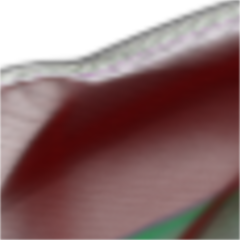
\includegraphics[width=1\textwidth]{../../Neue_Messungen/Supernova/cut/mdc_ors/mdc_ors_1.png}
		% \caption*{Quadrat 1 vergrößert dargestellt.}
		% \label{fig::res::sn_comp_mdc_ors_1}
	\end{minipage}
	\hfill
	\begin{minipage}[t]{0.3\textwidth}
		\centering
		
\includegraphics[width=1\textwidth]{../../Neue_Messungen/Supernova/cut/mdc_ors/mdc_ors_2.png}
		% \caption*{Quadrat 2 vergrößert dargestellt.}
		% \label{fig::res::sn_comp_mdc_ors_2}
	\end{minipage}
	\hfill
	\begin{minipage}[t]{0.3\textwidth}
		\centering
		
\includegraphics[width=1\textwidth]{../../Neue_Messungen/Supernova/cut/mdc_ors/mdc_ors_3.png}
		% \caption*{Quadrat 3 vergrößert dargestellt.}
		% \label{fig::res::sn_comp_mdc_ors_3}
	\end{minipage}
	\caption{Supernova mit MDC Raycast und variierter Strahlabtastrate berechnet.}
	\label{fig::res::sn_comp_mdc_ors}
\end{figure}

\begin{figure}[]
	\centering
	\begin{minipage}[t]{0.3\textwidth}
		\centering
		
\includegraphics[width=1\textwidth]{../../Neue_Messungen/Supernova/cut/ddc/ddc_1.png}
		% \caption*{Quadrat 1 vergrößert dargestellt.}
		% \label{fig::res::sn_comp_ddc_1}
	\end{minipage}
	\hfill
	\begin{minipage}[t]{0.3\textwidth}
		\centering
		
\includegraphics[width=1\textwidth]{../../Neue_Messungen/Supernova/cut/ddc/ddc_2.png}
		% \caption*{Quadrat 2 vergrößert dargestellt.}
		% \label{fig::res::sn_comp_ddc_2}
	\end{minipage}
	\hfill
	\begin{minipage}[t]{0.3\textwidth}
		\centering
		
\includegraphics[width=1\textwidth]{../../Neue_Messungen/Supernova/cut/ddc/ddc_3.png}
		% \caption*{Quadrat 3 vergrößert dargestellt.}
		% \label{fig::res::sn_comp_ddc_3}
	\end{minipage}
	\caption{Supernova mit DDC Raycast und ohne variierter Strahlabtastrate berechnet.}
	\label{fig::res::sn_comp_ddc}
\end{figure}

\begin{figure}[]
	\centering
	\begin{minipage}[t]{0.3\textwidth}
		\centering
		
\includegraphics[width=1\textwidth]{../../Neue_Messungen/Supernova/cut/ddc_ors/ddc_ors_1.png}
		% \caption*{Quadrat 1 vergrößert dargestellt.}
		% \label{fig::res::sn_comp_ddc_ors_1}
	\end{minipage}
	\hfill
	\begin{minipage}[t]{0.3\textwidth}
		\centering
		
\includegraphics[width=1\textwidth]{../../Neue_Messungen/Supernova/cut/ddc_ors/ddc_ors_2.png}
		% \caption*{Quadrat 2 vergrößert dargestellt.}
		% \label{fig::res::sn_comp_ddc_ors_2}
	\end{minipage}
	\hfill
	\begin{minipage}[t]{0.3\textwidth}
		\centering
		
\includegraphics[width=1\textwidth]{../../Neue_Messungen/Supernova/cut/ddc_ors/ddc_ors_3.png}
		% \caption*{Quadrat 3 vergrößert dargestellt.}
		% \label{fig::res::sn_comp_ddc_ors_3}
	\end{minipage}
	\caption{Supernova mit DDC Raycast und ohne variierter Strahlabtastrate berechnet.}
	\label{fig::res::sn_comp_ddc_ors}
\end{figure}

% \clearpage

\subsection{Performanz}
Für die Messung der Performanz der Implementierungen wurden zwei Messwerte bei einer Berechnung eines Bildes genommen.
Die Ausführungszeit des Kernels innerhalb einer Ausführung der \emph{paintGL()}-Methode und die Ausführungszeit der \emph{paintGL()}-Methode selbst.
Dies wurde deshalb so gewählt, da die Implementierungen nicht ausschließlich innerhalb des Kernels durchgeführt wurden, sondern auch außerhalb der Kernelaufrufe Programmcode geschrieben wurde und der Start einer Kernelausführung sowie die synchronisierte Beendigung eine gewisse Zeit brauchen.
Die Ausführungszeit der \emph{paintGL()}-Methode ist letztendlich der Wert, welcher die reale spürbare Performanz für den Nutzer angibt.

Für die Messungen der Performanz wurde kein Eyetracking verwendet, da dies lediglich die Mausposition mit der Blickposition ersetzt und keinen Einfluss auf die Ausführungszeit des Kernels und nur einen konstanten Einfluss auf die Ausführungszeit der \emph{paintGL()}-Methode hat.
Auch sollten, bei den Messungen mit den verschiedenen Methoden, möglichst die selben Mauspositionen verwendet werden, um vergleichbare Ergebnisse zu erhalten.
Die Verwendung eines Eyetrackers würde es fast unmöglich machen, die selben Blickpunkte in einem gewissen Zeitraum zu fokussieren.

Für die Messergebnisse selbst wurde ein spiegelverkehrtes \emph{S} mit dem Mauszeiger auf einem Bild geformt und dabei die Mauspositionen abgespeichert.
Insgesamt wurden hier 584 Mauspositionen aufgezeichnet.
Es wurden anschließend verschiedene Volumendaten mit jeweils drei verschiedenen Transferfunktionen für die drei verschiedenen Implementierungen, den Standard-, \emph{MDC}- und \emph{DDC}-Raycast sowie jeweils einmal mit konstanter und einmal mit variierter Strahlabtastrate für die Messungen verwendet.
Bei jeder dieser Messung wurde dabei für jede der Mauspositionen des gespeicherten Mausverlaufs ein Bild berechnet und zu dieser Berechnung die Mausposition, die Ausführungszeit des Kernels und die Ausführungszeit der \emph{paintGL()}-Methode gespeichert.

Die Hardware des Computers, mit welchem die Messungen durchgeführt wurden, besteht unter anderem aus einem \emph{Intel Core i5 4670k bei $3,40$\,GHz} CPU und einer \emph{GIGABYTE AMD Radeon (TM) R9 390 Series} GPU.
Die Auflösung der zu berechnenden Bilder betrug immer $2263\times1306$\,Pixel.

Die Messungen wurden mit den Volumen \emph{Bonsai}, \emph{Supernova} und \emph{Chameleon} durchgeführt.
Das Volumen \emph{Bonsai} hat eine Auflösung von $256\times256\times256$\,Voxel, wobei die Voxel eine Slice-Dicke von $1,0\times1,0\times1,0$ haben.
Das Volumen \emph{Supernova} hat eine Auflösung von $432\times432\times432$\,Voxel, wobei die Voxel eine Slice-Dicke von $1,0\times1,0\times1,0$ haben.
Das Volumen \emph{Chameleon} hat eine Auflösung von $1024\times1024\times1024$\,Voxel, wobei die Voxel eine Slice-Dicke von $0,09228515625\times0,09228515625\times0,105$ haben.

\begin{figure}
	\centering
	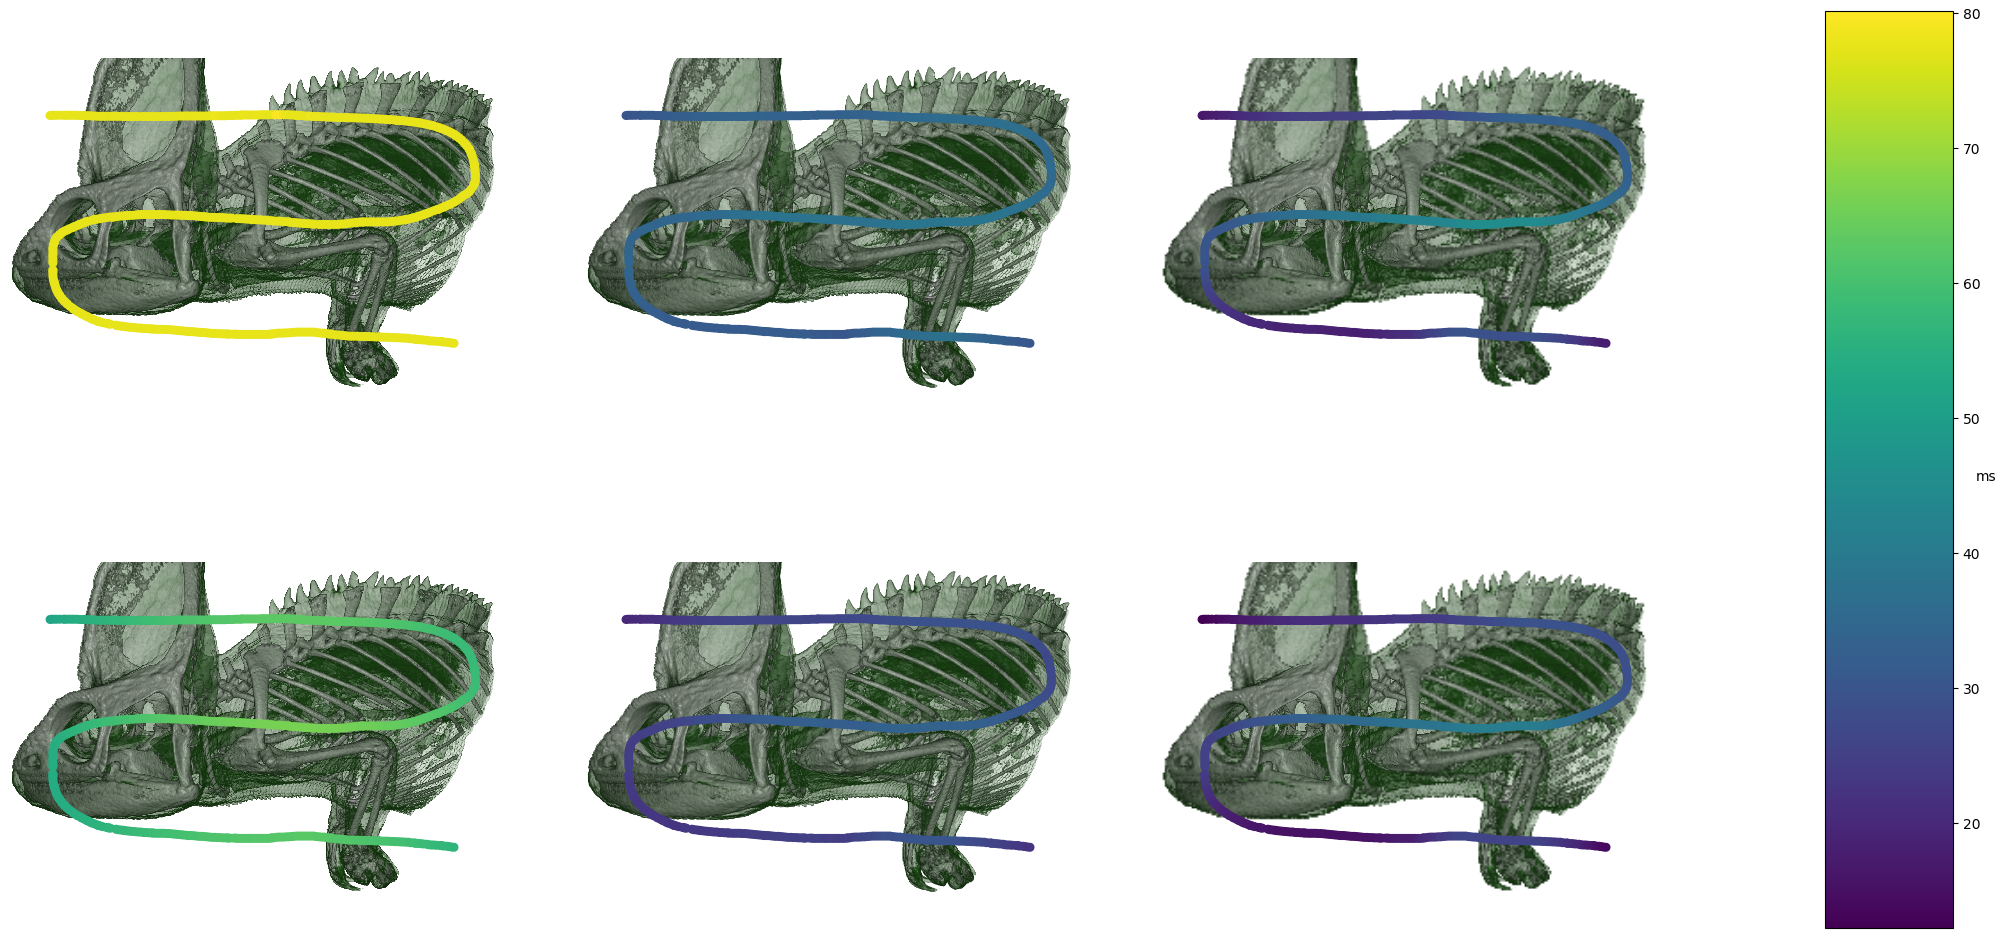
\includegraphics[width=1\textwidth]{../../Neue_Messungen/Chameleon/heatmaps/hm_wa.png}
	\caption{Heatmaps der verschiedenen Verfahren für das Volumen Chameleon. Für verschiedene Mauspositionen wurde eine Berechnung durchgeführt. Die jeweilige Ausführungszeit des Kernels für diese Berechnung wurde entsprechend des Farbbalkens farblich eingezeichnet. Der Farbbalken gibt die Werte in \,ms an. \emph{v. S. a. r.} steht für \emph{variierter Strahlabtastrate}}
	\label{fig::res::pf::hm_wa}
\end{figure}

Für einen anschaulichen Vergleich der Methoden wurde für die Messungen des Volumen Chameleon Heatmaps erstellt (Abbildung \ref{fig::res::pf::hm_wa}).
Die gemessene Ausführungszeiten des Kernels für die unterschiedlichen Mauspositionen wurden für die Erstellung der Heatmaps verwendet.
Da die Differenz zwischen Ausführungszeit des Kernels und der Ausführungszeit der \emph{paintGL()}-Methode unabhängig von dem zu berechnenden Volumen und der verwendeten Transferfunktion ist, wurde diese hier nicht einbezogen.

Abbildung \ref{fig::res::pf::hm_wa} zeigt, dass die Ausführungszeit des Kernels für den Standard Raycast ohne variierter Strahlabtastrate für alle Mauspositionen im Bereich von 80\,ms liegt und damit im Vergleich zu den anderen Methoden am höchsten ist.
Betrachtet man nun die Standard Variante mit variierter Strahlabtastrate, so kann man eine allgemeine Verbesserung feststellen.
Die Ausführungszeit des Kernels liegt bei dieser Methode bei circa 65\,ms und variiert je nach Mausposition leicht.
So ist die Ausführungszeit für eine Mausposition am oberen und unterem Rande des Bildes ein wenig geringer, als wenn diese sich in der Mitte des Bildes befindet.
Die Heatmap zur Methode mit dem MDC Raycast und ohne variierter Strahlabtastrate zeigt zu beiden Standard Raycast Methoden eine Verbesserung.
Die Ausführungszeit des Kernels liegt hier bei circa 40\,ms und ist im mittleren Bereich des Bildes minimal höher als im oberen oder unteren Bereich.
Wird der MDC Raycast mit einer variierten Strahlabtastrate kombiniert, so ist die Ausführungszeit des Kernels im oberen und unteren Bereich des Bildes sichtbar schneller, als in der Variante ohne einer variierten Strahlabtastrate.
Im mittleren Bereich des Bildes liegt sie nun bei circa 35\,ms und in den äußeren Bereichen des Bildes liegt sie bei circa 20\,ms.
Die Heatmap zum DDC Raycast zeigt, dass mit dem DDC Raycast je nach Mausposition die niedrigsten Ausführungszeit des Kernels erreicht wurde.
Auch ohne einer variierten Strahlabtastrate zeigt der DDC Raycast verhältnismäßig ein ähnliches Muster, wie der Standard und MDC Raycast mit variierter Strahlabtastrate.
Die Ausführungszeit des Kernels betrug hier im äußeren Bild ebenfalls geringere Werte als im mittigen Bereich des Bildes.
Im äußeren Bereich betrug sie circa 20\,ms und im mittleren circa 45\,ms.
Es ist auffallend, dass die Differenz zwischen der Ausführungszeit des Kernels im oberen und unteren Bereich und der Ausführungszeit im mittleren Bereich des Bildes hier größer als bei den anderen Verfahren ist.
In der Heatmap zum DDC Raycast mit variierter Strahlabtastrate ist zu erkennen, dass die äußeren Bereiche des Bildes, besonders oben links und unten rechts, nochmal niedrigere Ausführungszeiten des haben, als im DDC Raycast ohne variierter Strahlabtastrate.
In den äußeren Bereichen fällt diese auf bis zu 15\,ms und im mittleren Bereich auf leicht über 40\,ms.
Vergleicht man die Heatmaps des DDC und MDC Raycasts miteinander, so fällt auf, dass der DDC Raycast in den äußeren Bereichen des Bildes niedrigere Ausführungszeiten als der MDC Raycast erreicht, dafür die Ausführungszeiten des DDC Raycasts im mittleren Bereich des Bildes leicht höher ist, als die des MDC Raycasts.

Das die Ausführungszeiten im äußeren Bereich des Bildes geringer sind wird zwei unterschiedliche Gründe haben.
Erstens wird, wenn sich die Mausposition weiter weg von dem Volumen befindet, ein Großteil des Volumens beziehungsweise des Bildes mit einer geringeren Strahlabtastrate abgetastet, wodurch und einige Work-Items und Work-Groups früher terminieren können.
Zweitens ist die Bildabtastrate in der Nähe der Mausposition am höchsten.
Ist diese am Rande des Volumens, wie es in Abbildung \ref{fig::res::pf::hm_wa} auch der Fall ist, so fällt ein großer Anteil der Strahlen auf Bereiche, in denen nur wenige Voxel abgetastet werden müssen und dadurch wieder einige Work-Items und Work-Groups früher terminieren.
Das die MDC Methode ohne einer variierten Strahlabtastrate auch in den äußeren Bereichen eine relativ gleiche Ausführungszeit hat, wie in den inneren Bereichen des Volumens, wird daran liegen, dass der hoch aufgelöste innere Bereich des MDC Raycasts deutlich kompakter und ein wenig kleiner ist, als der des DDC Raycasts.
Dadurch fallen auch weniger Strahlen des hoch aufgelösten Bereichs außerhalb des Volumens, auch wenn sich die Mausposition am Rande des Volumens befindet.

\begin{figure}
	\centering
	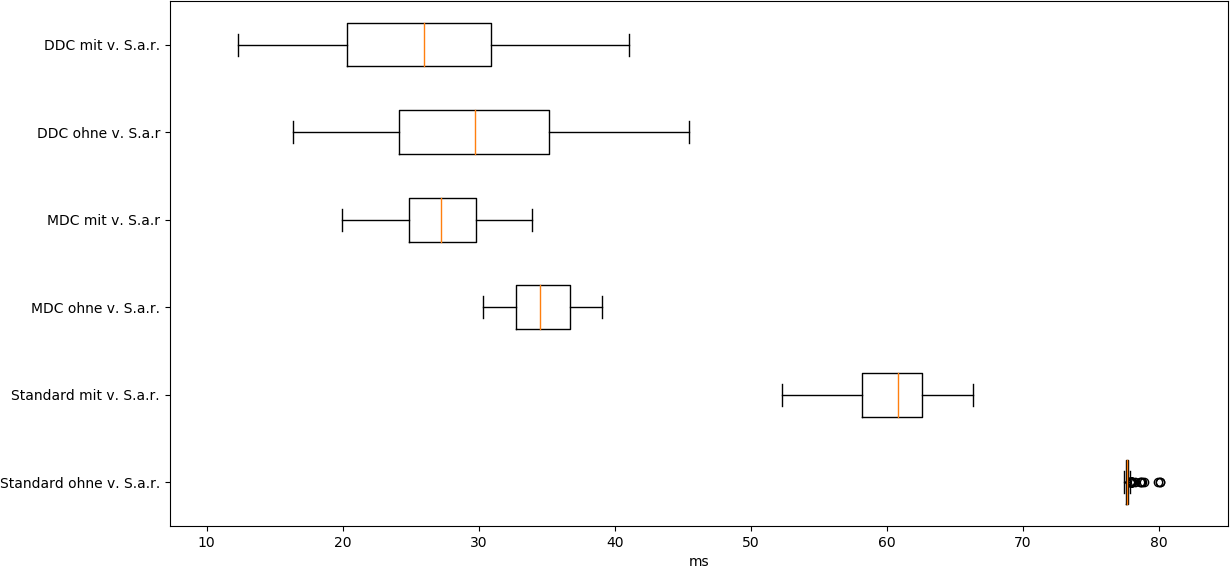
\includegraphics[width=1\textwidth]{../../Neue_Messungen/Chameleon/boxplots.png}
	\caption{Boxplots der Ausführungszeiten des Kernels der verschiedenen Verfahren bei der Verwendung des Volumen Chameleon. Die Box reicht von den unteren Viertel bis zu den oberen Viertel der Werte und der Median ist orange eingezeichnet.}
	\label{fig::res::pf::bp}
\end{figure}

Die Ausführungszeiten des Kernels der unterschiedlichen Methoden, wie sie in den Heatmaps (Abbildung \ref{fig::res::pf::hm_wa}) farbig dargestellt wurden, sind in Abbildung \ref{fig::res::pf::bp} als Boxplots dargestellt.
Wie an den Heatmaps schon ersichtlich war, sind die Ausführungszeiten des Standard Raycast ohne variierter Strahlabtastrate am höchsten und relativ gleich.
Die Messwerte sind konzentriert um die 77,5\,ms.
Die Ausführungszeiten für den Standard Raycast mit variierter Strahlabtastrate sind ein wenig geringer und sind untereinander stärker verteilt.
Für den MDC Raycast sieht es ähnlich aus.
Ohne variierter Strahlabtastrate sind die Werte ein wenig höher und dafür kompakter.
Mit einer variierten Strahlabtastrate sind sind die Werte niedriger aber weiter verteilt.
Anders wie bei den vorherigen Raycast Methoden sind die Ausführungszeiten des DDC Raycast mit variierter Strahlabtastrate ein wenig kompakter, als ohne variierter Strahlabtastrate.
Mit variierter Strahlabtastrate sind die Werte insgesamt aber trotzdem niedriger.

\begin{table}
	\centering
	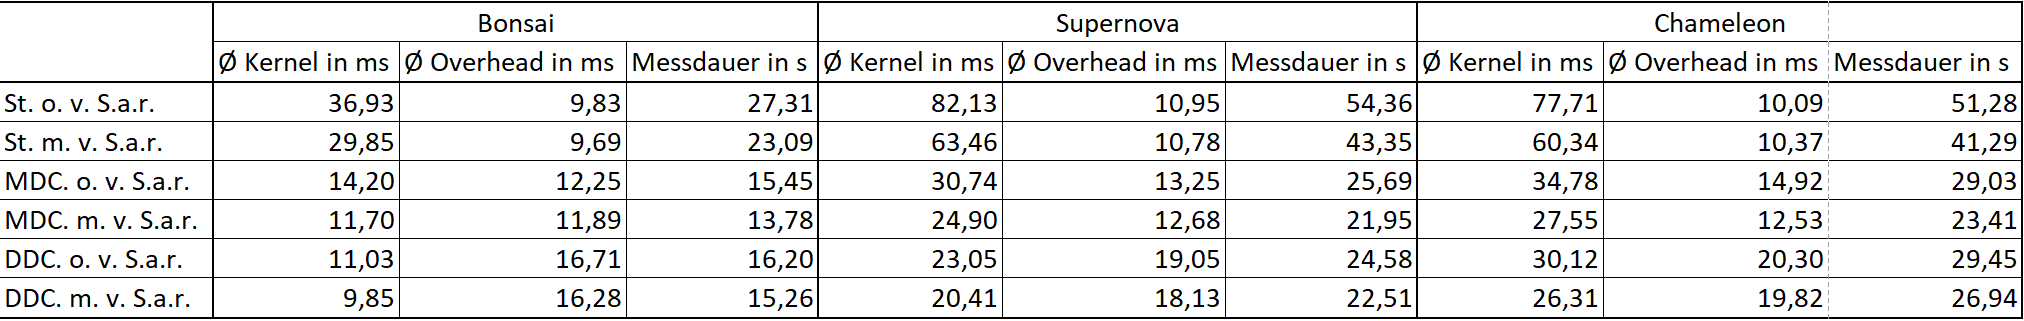
\includegraphics[width=1\textwidth]{../../Neue_Messungen/Messungen_in_Tabelle.PNG}
	\caption{Die Ergebnisse der verschiedenen Verfahren mit den Volumen Bonsai, Supernova und Chameleon. Für jedes Verfahren und Volumen ist die durchschnittliche Ausführungszeit des Kernel (K.) und die Varianz von dieser sowie der durchschnittliche Overhead (Oh.) und die summierte Ausführungszeit der \emph{paintGL()}-Methode (Md.) für die verschiedenen Mauspositionen angegeben.}
	\label{fig::res::pf::table}
\end{table}

Wie schon in Abbildung \ref{fig::res::pf::hm_wa} und \ref{fig::res::pf::bp} die Verhältnisse der Ausführungszeiten der verschiedenen Methoden dargestellt wurden, wird dies in Tabelle \ref{fig::res::pf::table} durch die genauen Werte bestätigt.
In Tabelle \ref{fig::res::pf::table} sind für die unterschiedlichen Verfahren und die Volumen Bonsai, Supernova und Chameleon die durchschnittliche Kernelzeit, dessen Varianz sowie der durchschnittliche Overhead der \emph{paintGL()}-Methode ohne die Ausführungszeit des Kernels dargestellt.
Zusätzlich ist auch die summierte Ausführungszeit der \emph{paintGL()}-Methode für die insgesamt 584 verschiedenen Berechnungen jeder Messung angegeben.

Betrachtet man den Overhead der verschiedenen Methoden, so sieht man, dass der Standard Raycast für die unterschiedlichen Volumen ähnlich ist und mit circa 10\,s den geringsten Overhead hat.
Die Implementierung des Standard Raycasts verwendet auch nur einen Kernel Aufruf.
Der Overhead des MDC Raycasts ist ein wenig höher als der des Standard Raycasts und beträgt für das Bonsai Volumen circa 12\,s, für das Supernova Volumen circa 13\,s und für das Chameleon Volumen circa 14\,s.
Der Overhead des DDC Raycasts ist am höchsten und beträgt für den Bonsai circa 16\,s, für die Supernova circa 19\,s und für das Chameleon circa 20\,s.
Sowohl der MDC Raycast als auch der DDC Raycast verwenden jeweils zwei Kernel Aufrufe aber der DDC Raycast berechnet vor der Ausführung des Kernels noch einige Werte, die für diesen Raycast benötigt werden.

Vergleicht man die verschiedenen Volumen, so wird das Bonsai Volumen deutlich schneller als das Supernova oder Chameleon Volumen berechnet.
Dies wird hauptsächlich an der geringeren Auflösung des Volumens und damit einer deutlich geringeren Anzahl an Voxeln liegen.
Im Widerspruch dazu benötigt aber die Messung für das Supernova Volumens etwas länger, als die Messung für das Chameleon Volumen.
Die Wahl der Transferfunktion in Verbindung mit dem in allen Raycasts vorimplementierten \emph{Empty-Space-Skipping (ESS)} könnte hier eine Rolle spielen.
Werden in einem Volumen die Voxel nicht vollständig transparent gemacht, sondern haben immer noch einen gewissen Opazitätswert, so werden diese nicht durch das ESS übersprungen, was zu einer längeren Berechnung führt.
Ein weiterer Grund ist kann die Perspektive auf die Volumen sein.
Das Chameleon Volumen wird von der Seite betrachtet und hat aufgrund der nicht einheitlichen Slice-Dicken eine geringere Tiefe, wenn man es von der Seite betrachtet.
Daher terminieren die Strahlen von der Seite früher.
Das Supernova Volumen hingegen ist relativ rund und hat eine einheitlich Slice-Dicke.

\section{Diskussion}\label{sec::disc}
Betrachtet man rückblickend auf die Ergebnisse die unterschiedlichen Bildabtastraten, so ist es offensichtlich, dass der Standard Raycast von den unterschiedlichen Methoden her, die beste Bildqualität erzeugt.
Trotzdem kann durch das Ausnutzen der Limitierungen des visuellen Wahrnehmungssystems des Menschen bei der Verwendung eines Eyetrackers annähernd der Effekt erzeugt werden, dass die Raycast Methoden MDC und DDC das Bild in voller Auflösung berechnen, obwohl dies nicht der Fall.
Da die Auflösung beim MDC Raycast im äußeren Bereich im Vergleich zum DDC Raycast immer noch deutlich höher ist, ist dieser Effekt für den MDC Raycast viel realistischer und kaum wahrnehmbar während beim DDC Raycast noch Artefakte des am niedrigsten aufgelösten Bereichs wahrnehmbar sind.
Um die Bildqualität des DDC Raycasts weiter zu verbessern, könnte die Bildabtastrate des äußersten Bereichs angehoben und oder der Radius des mittleren Bereichs vergrößert werden, so dass die reduzierte Auflösung noch weniger auffällt.
Für den MDC Raycast hingegen wäre es denkbar, die Auflösung des äußeren Bereichs selbst weiter zu verringern oder einen zusätzlichen Bereich einzufügen, der nur noch ein Achtel der maximalen Auflösung hat.

Betrachtet man rückblickend auf die Ergebnisse die unterschiedlichen Varianten, mit variierter und ohne variierter Strahlabtastrate, so gibt es hier bei den Bildern kaum wahrnehmbare Unterschiede.
Im Gegensatz zu den statischen Bildern wurde aber bei aktivem Eyetracking bei den Varianten mit variierter Strahabtastrate, Artefakte durch die veränderte Strahlabtastrate im Bild wahrgenommen, wenn sich die Augen über das Bild bewegt haben.
Während einer Fixation verblassen diese Artefakte und sind wie bei einem statischen Bild kaum mehr wahrnehmbar.
Die Ergebnisse scheinen anzudeuten, dass die Strahlabtastrate im äußeren Bereich noch weiter reduziert werden könnte, da diese bisher nur auf ein Minimum von ein Viertel der normalen Strahlabtastrate nach außen hin fallen kann.
In weiteren Tests hat das Reduzieren des Limits auf ein Fünftel schon deutlich Artefakte der Unterabtastung ergeben, die dafür aber auch nur an den vom Blickpunkt entferntesten Stellen aufgetreten sind und daher nicht so aufgefallen sind.
Weiter wäre es denkbar, die Funktion, die die Strahlabtastrate abhängig von der Distanz zur Mausposition anpasst, abzuändern, so dass diese schon bei einer geringeren Entfernung stärker abnimmt und früher das Limit erreicht.
Da selbst bei nur einem Viertel der maximalen Strahlabtastrate im äußeren Bereich kaum Artefakte wahrnehmbar sind, sollte dies ohne eine wahrnehmbare Reduzierung der Bildqualität möglich sein.

Hinsichtlich der Ausführungszeit des Kernels zeigen die Ergebnisse deutlich, dass der Standard Raycast ohne variierter Strahlabtastrate am schlechtesten abschneidet.
Der MDC Raycast ohne variierter Strahlabtastrate ist hier besser und hat aber eine höhere Varianz.
Der DDC Raycast ebenfalls ohne variierter Strahlabtastrate erreicht deutlich geringere Kernelausführungszeiten als der MDC Raycast und hat einen niedrigeren Median und Durchschnitt.
Dafür erreicht der DDC Raycast im Vergleich zum MDC Raycast aber auch deutlich höhere Kernelausführungszeiten und hat daher auch eine deutlich höhere Varianz.
Wird zusätzlich zu den verschiedenen Methoden eine variierte Strahlabtastrate verwendet, so verringert sich bei allen Methoden die Kernelausführungszeiten und bis auf den DDC Raycast, bei dem sich die Varianz dadurch ein wenig verringert hat, hat sich beim Standard und MDC Raycast die Varianz dadurch erhöht.

Hinsichtlich der wahrgenommenen Performanz, also der Ausführungszeiten inklusive des Overheads, schneidet der MDC Raycast trotz einer höheren durchschnittlichen Kernelausführungszeit aufgrund des geringeren Overheads besser ab, als der DDC Raycast.
Da zusätzlich die Varianz des MDC Raycasts geringer ist und dies daher auch bei der Verwendung eines Eyetrackers zu weniger Verzögerungen führt, als beim DDC Raycasts sowie der MDC Raycast bei Mauspositionen, die sich innerhalb des Volumens befinden, sich besser verhält, ist aus Sicht der Performanz der MDC Raycast mit variierter Strahlabtastrate die beste Wahl.
Da zusätzlich der MDC Raycast höherwertige Bilder als der DDC Raycast generiert, trotzdem der Verlust der Bildqualität bei der Verwendung eines Eyetrackers im Vergleich zum Standard Raycast nicht wahrnehmbar ist, schneidet der MDC Raycast mit variierter Strahlabtastrate in Verbindung mit einem Eyetracker von den verschiedenen Methoden her insgesamt am besten ab.

Dass der MDC Raycast von der Performanz her besser abschneidet als der DDC Raycast liegt an unterschiedlichen Faktoren.
So ist wie genannt, der Overhead ein wichtiger Faktor, der die wahrnehmbare Performanz des DDC Raycasts im Vergleich zum MDC Raycast beeinträchtigt.
Ein weiterer Faktor ist die Umsetzung des Index-Mappings.
Aufgrund dessen, dass dieses versucht wurde variabel zu halten, wurden viele Berechnungen für das Abbilden der Indizes durchgeführt, bevor der eigentliche Raycast beginnt.
Die Work-Items werden hier anhand ihrer globalen ID auf völlig unterschiedliche Bildkoordinaten abgebildet.
Dies passiert unabhängig davon, in welcher Work-Group sie sich befinden, wodurch unter Umständen sehr unterschiedliche Bereiche durch eine Work-Group berechnet werden und die gesamte Work-Group immer auf das langsamste Work-Item warten muss.
Eine Änderung der Implementierung dahingehend, dass die Work-Items nicht anhand der globalen ID sondern anhand der Work-Group ID mit der gesamten Work-Group auf einen zusammen liegenden Block von Bildkoordinaten abgebildet werden, würde die Ausführungszeit vieler Work-Groups verbessern.
Ein anderer Faktor ist die Art und Weise, wie die NDRange des Kernels festgelegt wird.
Eine Anpassung dieser, dass sie in mindestens eine Dimension ein Vielfaches der Work-Group Größe ist, würde die Anzahl zu startender Work-Groups reduzieren und die Ausführungszeit des Kernels weiter verbessern.
Die hohe Varianz des DDC Raycasts liegt vermutlich also vor allem an der Art der Implementierung.
Eine Optimierung dieser Implementierung würde sowohl die Ausführungszeit des Kernels, als auch den Overhead reduzieren, so dass der DDC Raycast insgesamt eine bessere Performanz als der MDC Raycast hat.

% Zusammenfassung und Ausblick
% % Fazit der Arbeit
\chapter{Fazit}\label{chap:zusfas}
\todo{Fazit wertend (was hat gut und schlecht funktioniert aber auf den gesamten Zeitverlauf der Arbeit bezogen).}
% Einarbeitung in das Projekt aufwendig, da die programmiersprache(n)-, umgebung und verwendeten bibliotheken unbekannt
% Grundlagenteil, hilfreich, vor allem GPU Architketur sehr interessant und hilfreich bei der implementierung des raycasts. trotzdem wie in diskussion herausgestellt, kann man oft noch dinge optimieren und man muss auf bestimmte eigenschaften achten.
% Die Auseinandersetzung mit den Eignschaften des Sehapparates war wichtig für das Grundlegende Verständniss, man könnte dahingehend aber noch genauere untersuchungen und messungen machen, z.b. die exakte größe des normal aufgelösten bereichs auf die refernenzwerte für die wahrnehmung anpassen
% Volumenrendering mit Raycast gut möglich, ermöglicht auch viele erweiterungen und modifikationen des Volumenrenderings, wie wahrnehmungsorientierte eigenschaften, reduzierung der strahlabtastrate, aber im Referenzliteraturteil auch gesehen, dass wahrnehmungsorientiert auch mit Rastergrafik möglich ist und vll. Volumenrendering mit Rastergrafik auch durchfürbar
% Einen Entwurf anzufertigen mit Arbeitspaketen, die durchgesetzt werden sollen, war hilfreich da man sich daran halten konnte und ermöglichte eine gewisse einteilung der arbeit
% Bezogen auf die Ergebnisse hat es gezeigt, dass wahrnehmungsorientierte methoden durchaus einen performanzgewinn bringen können ohne die bildqualität zu beeinträchtigen.
% Alleine die Anpassung der Strahlabtastrate hat kaum wahrnehmbare Bildqualitative Veränderungen nach sich gezogen und trotzdem die Ausführungszeit spürbar verbessert.
% Die anpassungen der Bildabtastrate gab es zwei Methoden, mdc ddc
% mdc der einfachere umgesetzte ansatz und ging von der implementierung her auch deutlich schneller
% trotzdem mdc it sar insgesamt am besten abgeschnitten, sowohl performanz als auch deutlich besser in der bildqualität als ddc
% den ansatz, der bei mdc gegangen wurde könnte man daher weiter ausbauen, z.B. bildabtastrate im äußeren bereich weiter verringern und u.U. einen dritten bereich einfügen, solange der Overhead dadurch nicht zu groß wird, da bisher im vergleich mdc hauptsächlich wegem dem overhead bessere werte gezeigt hat
% ddc war deutlich zeitaufwendiger zu implementieren, da index hinund her gemappt wurden und anschließend noch eine interpolation benötigt wurde
% ddc hat bessere spitzenwerte aber ist von der Performanz her aufgrund des overheads schlechter als mdc
% auch die Bildqualität leidet unter der niedrigen Bildabtastrate, wird aber aufgrund der limitationen des visuellen wahrnehmungssystems bei der verwendung eines eyetrackers lange nicht so wahrgenommen, wie wenn man nur das statische Bild betrachtet, ohne einen Eyetracker
% ddc ist wie in diskussion schon erwähnt ausbaufähig und kann vermutlich bei einer besseren umsetzung deutlich effizienter werden und aufgrund des einzelnen raycasts auch vom overhead schneller werden.
% Im Vergleich zur Referenzliteratur, in welcher deutlich höhere Faktoren in der Performanzgewinnung erfahren wurden, liegt dies unter anderem auch daran, dass die raycast methoden vor allem die ddc methode in der implementierung möglichst variabel gehalten wurde und auch daran, dass wie schon erwähnt in den implementierungen hier noch genügend verbesserungsmöglichkeiten existieren.
% Ein interessanter Ansatz für die Zukunft, wäre eine implementierung die wie eine Art Linse (verweis überlegung im arbeitspaket), die die Strahldichte gleichmäßig reduzieren kann
% Bezogen Auf die Arbeit mit dem Eyetracker war es sehr interessant damit zu arbeiten.
% Dass die api eine validierung der augendaten zur verfügung stellt hat sehr geholfen. Insgesamt ist aber bei der Arbeit mit dem Eyetracker noch aufgefallen, dass es entweder durch die Tremor-Bewegungen des Auges oder durch Messungenauigkeiten des Eyetrackers zu einem Flackern kommt. Da das Bild auf das Flackern reagiert ziehen sich veränderte Eigenschaften die Aufmerksamkeit auf sich und dadurch wirkt das Bild ein wenig störend. Für eine weitere Arbeit mit Eyetracking Daten sollten diese gefiltert oder geglättet werden.
% Abschließend ist zu sagen, dass sowohl die vorgestellten Methoden als auch wahrnehmungs-orientiertes Rendering hohes Potential hat und aufgrund der größeren Bildschirme und Pixeldichten vor allem auch in VR-Anwendungen, die nicht immer mit high-end hardware ausgestattet sind, dies auch in zukunft einen wichtigen aspekt haben wird.
% Ausserdem ist die Performanz nicht der einzige Grund für wahrnehmungsorientiertes Rendering. Wie auch in der Referenzliteratur beschrieben, kann dieses auch für Informativere Darstellungen sorgen. Oder auch die Augenbewegungen für die Steuerung von Anwendungen verwenden.


\printbibliography

%Alle URLs wurden zuletzt am 17.\,03.\,2018 geprüft.

%\renewcommand{\appendixtocname}{Anhang}
%\renewcommand{\appendixname}{Anhang}
%\renewcommand{\appendixpagename}{Anhang}
\appendix
%% !TeX root = main-german.tex
% !TeX spellcheck = de_DE
% !TeX encoding = utf8
% -*- coding:utf-8 mod:LaTeX -*-

%Die Angabe des schlauen Spruchs auf diesem Wege funtioniert nur,
%wenn keine Änderung des Kapitels mittels den in preambel/chapterheads.tex
%vorgeschlagenen Möglichkeiten durchgeführt wurde.
\setchapterpreamble[u]{%
  \dictum[Albert Einstein]{Probleme kann man niemals mit derselben Denkweise lösen, durch die sie entstanden sind.}
}
\chapter{LaTeX-Tipps}
\label{chap:latextipps}

In diesem Kapitel sollen allgemeine \LaTeX-Hinweise gegeben werden.

\section{Trennung von Absätzen}

Pro Satz eine neue Zeile.
Das ist wichtig, um sauber versionieren zu können.
In LaTeX werden Absätze durch eine Leerzeile getrennt.
Analogie zu Word: Bei Word werden neue Absätze durch einmal Eingabetaste gemacht.
Dies führt bei LaTeX jedoch nicht zu einem neuen Absatz, da LaTeX direkt aufeinanderfolgende Zeilen zu einer Zeile zusammenfügt.
Möchte man nun einen Absatz haben, muss man zweimal die Eingabetaste drücken.
Dies führt zu einer leeren Zeile.
In Word gibt es die Funktion Großschreibetaste und Eingabetaste gleichzeitig.
Wenn man dies drückt, wird einer harter Umbruch erzwungen.
Der Text fängt am Anfang der neuen Zeile an.
In LaTeX erreicht man dies durch Doppelbackslashes (\textbackslash\textbackslash) erzeugt.
Dies verwendet man quasi nie.

Folglich werden neue Abstäze insbesondere \emph{nicht} durch Doppelbackslashes erzeugt.
Beispielsweise begann der letzte Satz in einem neuen Absatz.
Eine ausführliche Motivation hierfür findet sich in \url{http://loopspace.mathforge.org/HowDidIDoThat/TeX/VCS/#section.3}.

Möchte man die Art des Absatzes ändern, so kann man die Dokumentklassenoption \texttt{parskip} verwenden.
Beispielsweise kann man mit \texttt{parskip=off} erreichen, dass statt eines freien Bereichs die erste Zeile des Absatzes eingezogen wird.

\section{File-Encoding und Unterstützung von Umlauten}
\label{sec:firstsectioninlatexhints}
Die Vorlage wurde 2010 auf UTF-8 umgestellt.
Alle neueren Editoren sollten damit keine Schwierigkeiten haben.

\section{Zitate}
Referenzen werden mittels \texttt{\textbackslash cite[key]} gesetzt.
Beispiel: \cite{WSPA} oder mit Autorenangabe: \citet{WSPA}.

Der folgende Satz demonstriert 
\begin{filecontents*}{\democodefile}
\begin{inparaenum}[1.]
  \item die Großschreibung von Autorennamen am Satzanfang,
  \item die richtige Zitation unter Verwendung von Autorennamen und der Referenz,
  \item dass die Autorennamen ein Hyperlink auf das Literaturverzeichnis sind sowie
  \item dass in dem Literaturverzeichnis der Namenspräfix \qq{van der} von \qq{Wil M.\,P.\ van der Aalst} steht.
\end{inparaenum}
\end{filecontents*}

\PrintDemo{style=parallel}

\Citet{RVvdA2016} präsentieren eine Studie über die Effektivität von Workflow-Management-Systemen.

Der folgende Satz demonstriert, dass man mittels \texttt{label} in einem Bibliopgrahie"=Eintrag den Textteil des generierten Labels überschreiben kann, aber das Jahr und die Eindeutigkeit noch von biber generiert wird.
Die Apache ODE Engine \cite{ApacheODE} ist eine Workflow-Maschine, die \BPEL-Prozesse zuverlässig ausführt.

Wörter am besten mittels \texttt{\textbackslash qq\{...\}} \qq{einschließen}, dann werden die richtigen Anführungszeichen verwendet.

Beim Erstellen der Bibtex-Datei wird empfohlen darauf zu achten, dass die DOI aufgeführt wird.

\section{Mathematische Formeln}
\label{sec:mf}
Mathematische Formeln kann man $so$ setzen. \texttt{symbols-a4.pdf} (zu finden auf \url{http://texdoc.net/pkg/symbols-a4}) enthält eine Liste der unter LaTeX direkt verfügbaren Symbole.
Beispielsweise $\mathbb{N}$ für die Menge der natürlichen Zahlen.
Für eine vollständige Dokumentation für mathematischen Formelsatz sollte die Dokumentation zu \texttt{amsmath}, \url{http://texdoc.net/pkg/amsmath} gelesen werden.

Folgende Gleichung erhält keine Nummer, da \texttt{\textbackslash equation*} verwendet wurde.
\begin{filecontents*}{\democodefile}
\begin{equation*}
  x = y
\end{equation*}
\end{filecontents*}

\PrintDemo{style=parallel}

Die Gleichung~\ref{eq:test} erhält eine Nummer:
\begin{filecontents*}{\democodefile}
\begin{equation}
  \label{eq:test}
  x = y
\end{equation}
\end{filecontents*}

\PrintDemo{style=parallel}

Die Vorlage bietet \verb+\abs+ an, damit die Absolutbetragsstriche richtig skalieren:
$\abs{X}$.

Eine ausführliche Anleitung zum Mathematikmodus von LaTeX findet sich in \url{http://www.ctan.org/tex-archive/help/Catalogue/entries/voss-mathmode.html}.

\section{Quellcode}
\Cref{lst:ListingANDlstlisting,helloworld} zeigen, wie man Programmlistings einbindet.
Mittels \texttt{\textbackslash lstinputlisting} kann man den Inhalt direkt aus Dateien lesen.

%Listing-Umgebung wurde durch \newfloat{Listing} definiert

\begin{Listing}
  \begin{lstlisting}[language=XML]
<listing name="second sample">
  <!-- comment -->
  <content>not interesting</content>
</listing>
\end{lstlisting}
  \caption{lstlisting in einer Listings-Umgebung, damit das Listing durch Balken abgetrennt ist}
  \label{lst:ListingANDlstlisting}
\end{Listing}


%TODO: Currently not shown in TOC
\lstinputlisting[language=C++,label=helloworld,caption={"`hello world"' in C++.},float]{code/helloworld.cpp}

Quellcode im \lstinline|<listing />| ist auch möglich.


\section{Pseudocode}
\Cref{alg:sample} zeigt einen Beispielalgorithmus.


\begin{Algorithmus} %Die Umgebung nur benutzen, wenn man den Algorithmus ähnlich wie Graphiken von TeX platzieren lassen möchte
  \caption{Sample algorithm}
  \label{alg:sample}
  %EN: This is an environment from the algorithmicx package
  \begin{algorithmic}
    \Procedure{Sample}{$a$,$v_e$}
      \State $\mathsf{parentHandled} \gets (a = \mathsf{process}) \lor \mathsf{visited}(a'), (a',c,a) \in \mathsf{HR}$
      \State \Comment $(a',c'a) \in \mathsf{HR}$ denotes that $a'$ is the parent of $a$
    \If{$\mathsf{parentHandled}\,\land(\mathcal{L}_\mathit{in}(a)=\emptyset\,\lor\,\forall l \in \mathcal{L}_\mathit{in}(a): \mathsf{visited}(l))$}
      \State $\mathsf{visited}(a) \gets \text{true}$
      \State $\mathsf{writes}_\circ(a,v_e) \gets
        \begin{cases}
          \mathsf{joinLinks}(a,v_e)                & \abs{\mathcal{L}_\mathit{in}(a)} > 0 \\
          \mathsf{writes}_\circ(p,v_e)
                                                   & \exists p: (p,c,a) \in \mathsf{HR}   \\
          (\emptyset, \emptyset, \emptyset, false) & \text{otherwise}
        \end{cases}
      $
    \If{$a\in\mathcal{A}_\mathit{basic}$}
      \State \Call{HandleBasicActivity}{$a$,$v_e$}
    \ElsIf{$a\in\mathcal{A}_\mathit{flow}$}
      \State \Call{HandleFlow}{$a$,$v_e$}
    \ElsIf{$a = \mathsf{process}$} \Comment Directly handle the contained activity
      \State \Call{HandleActivity}{$a'$,$v_e$}, $(a,\bot,a') \in \mathsf{HR}$
      \State $\mathsf{writes}_\bullet(a) \gets \mathsf{writes}_\bullet(a')$
    \EndIf
    \ForAll{$l \in \mathcal{L}_\mathit{out}(a)$}
      \State \Call{HandleLink}{$l$,$v_e$}
    \EndFor
    \EndIf
    \EndProcedure
  \end{algorithmic}
\end{Algorithmus}

\clearpage
Und wer einen Algorithmus schreiben möchte, der über mehrere Seiten geht, der kann das nur mit folgendem \textbf{üblen} Hack tun:

{
\begin{minipage}{\textwidth}
  \hrule height .8pt width\textwidth
  \vskip.3em%\vskip\abovecaptionskip\relax
  \stepcounter{Algorithmus}
  \addcontentsline{alg}{Algorithmus}{\protect\numberline{\theAlgorithmus}{\ignorespaces Description \relax}}
  \noindent\textbf{Algorithmus \theAlgorithmus} Description
  %\stepcounter{algorithm}
  %\addcontentsline{alg}{Algorithmus}{\thealgorithm{}\hskip0em Description}
  %\textbf{Algorithmus \thealgorithm} Description
  \vskip.3em%\vskip\belowcaptionskip\relax
  \hrule height .5pt width\textwidth
\end{minipage}
%without the following line, the text is nerer at the rule
\vskip-.3em
%
code goes here\\
test2\\
%
\vskip-.7em
\hrule height .5pt width\textwidth
}




\section{Abbildungen}

Die \cref{fig:chor1} und \ref{fig:chor2} sind für das Verständnis dieses Dokuments wichtig.
Im Anhang zeigt \vref{fig:AnhangsChor} erneut die komplette Choreographie.

%Die Parameter in eckigen Klammern sind optionale Parameter - z.B. [htb!]
%htb! bedeutet: "Liebes LaTeX, bitte platziere diese Abbildung zuerst hier ("_h_ere"). Falls das nicht funktioniert, dann bitte oben auf der Seite ("_t_op"). Und falls das nicht geht, bitte unten auf der Seite ("_b_ottom"). Und bitte, bitte bevorzuge hier und oben, auch wenn's net so optimal aussieht ("!")
%Diese sollten nach Möglichkeit NICHT verwendet werden. LaTeX's Algorithmus für das Platzieren der Gleitumgebung ist schon sehr gut!

\begin{figure}
  \centering
  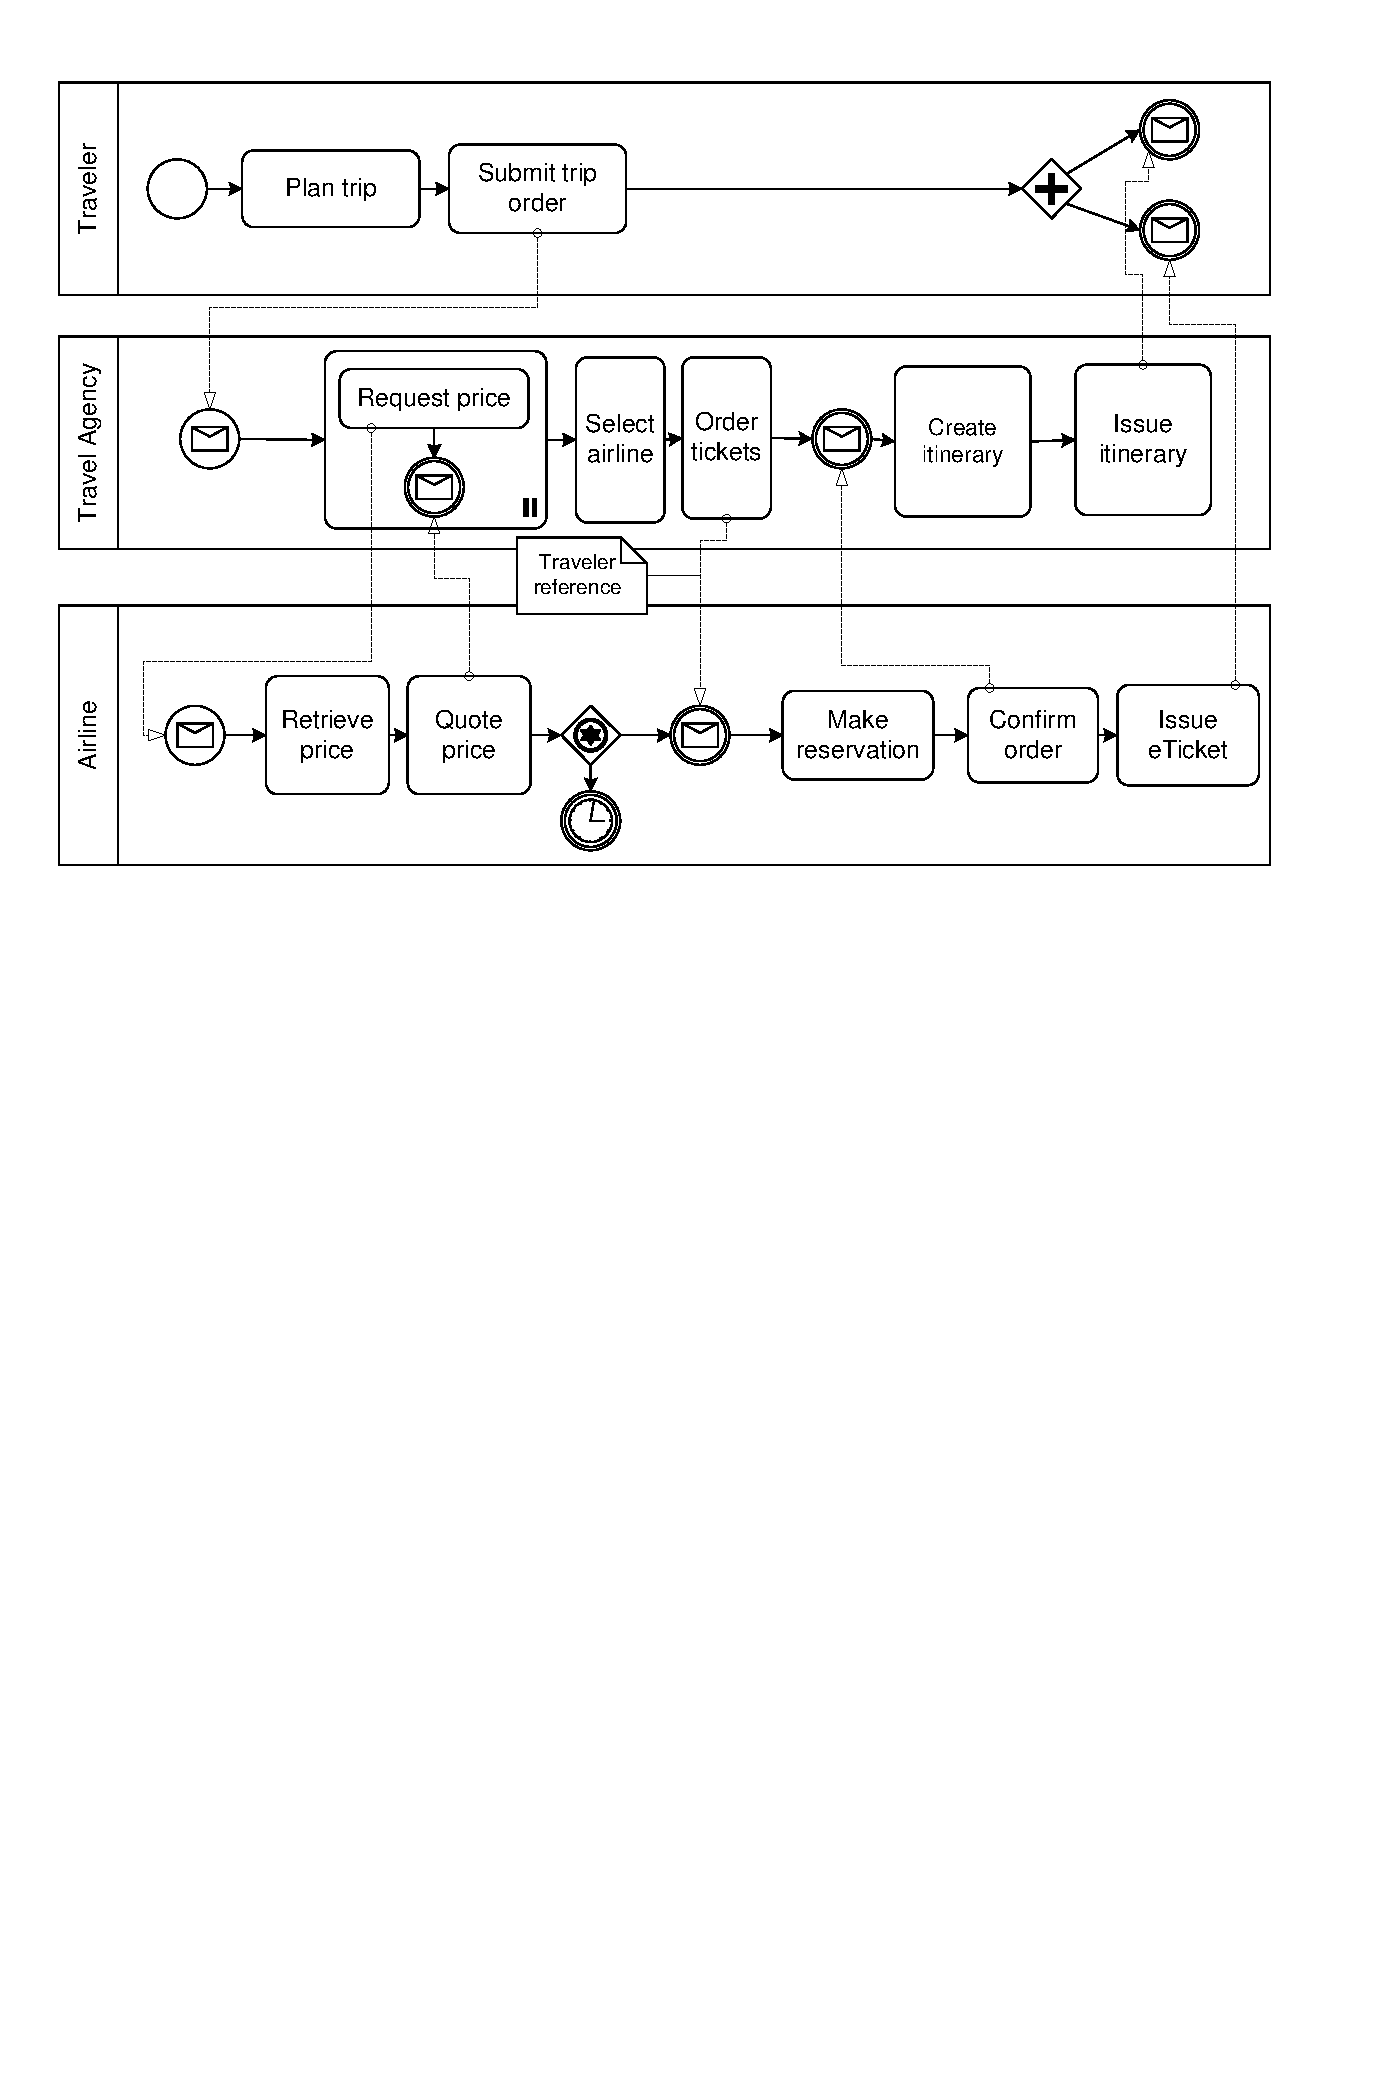
\includegraphics[width=\textwidth]{choreography.pdf}
  \caption{Beispiel-Choreographie}
  \label{fig:chor1}
\end{figure}



\begin{figure}
  \centering
  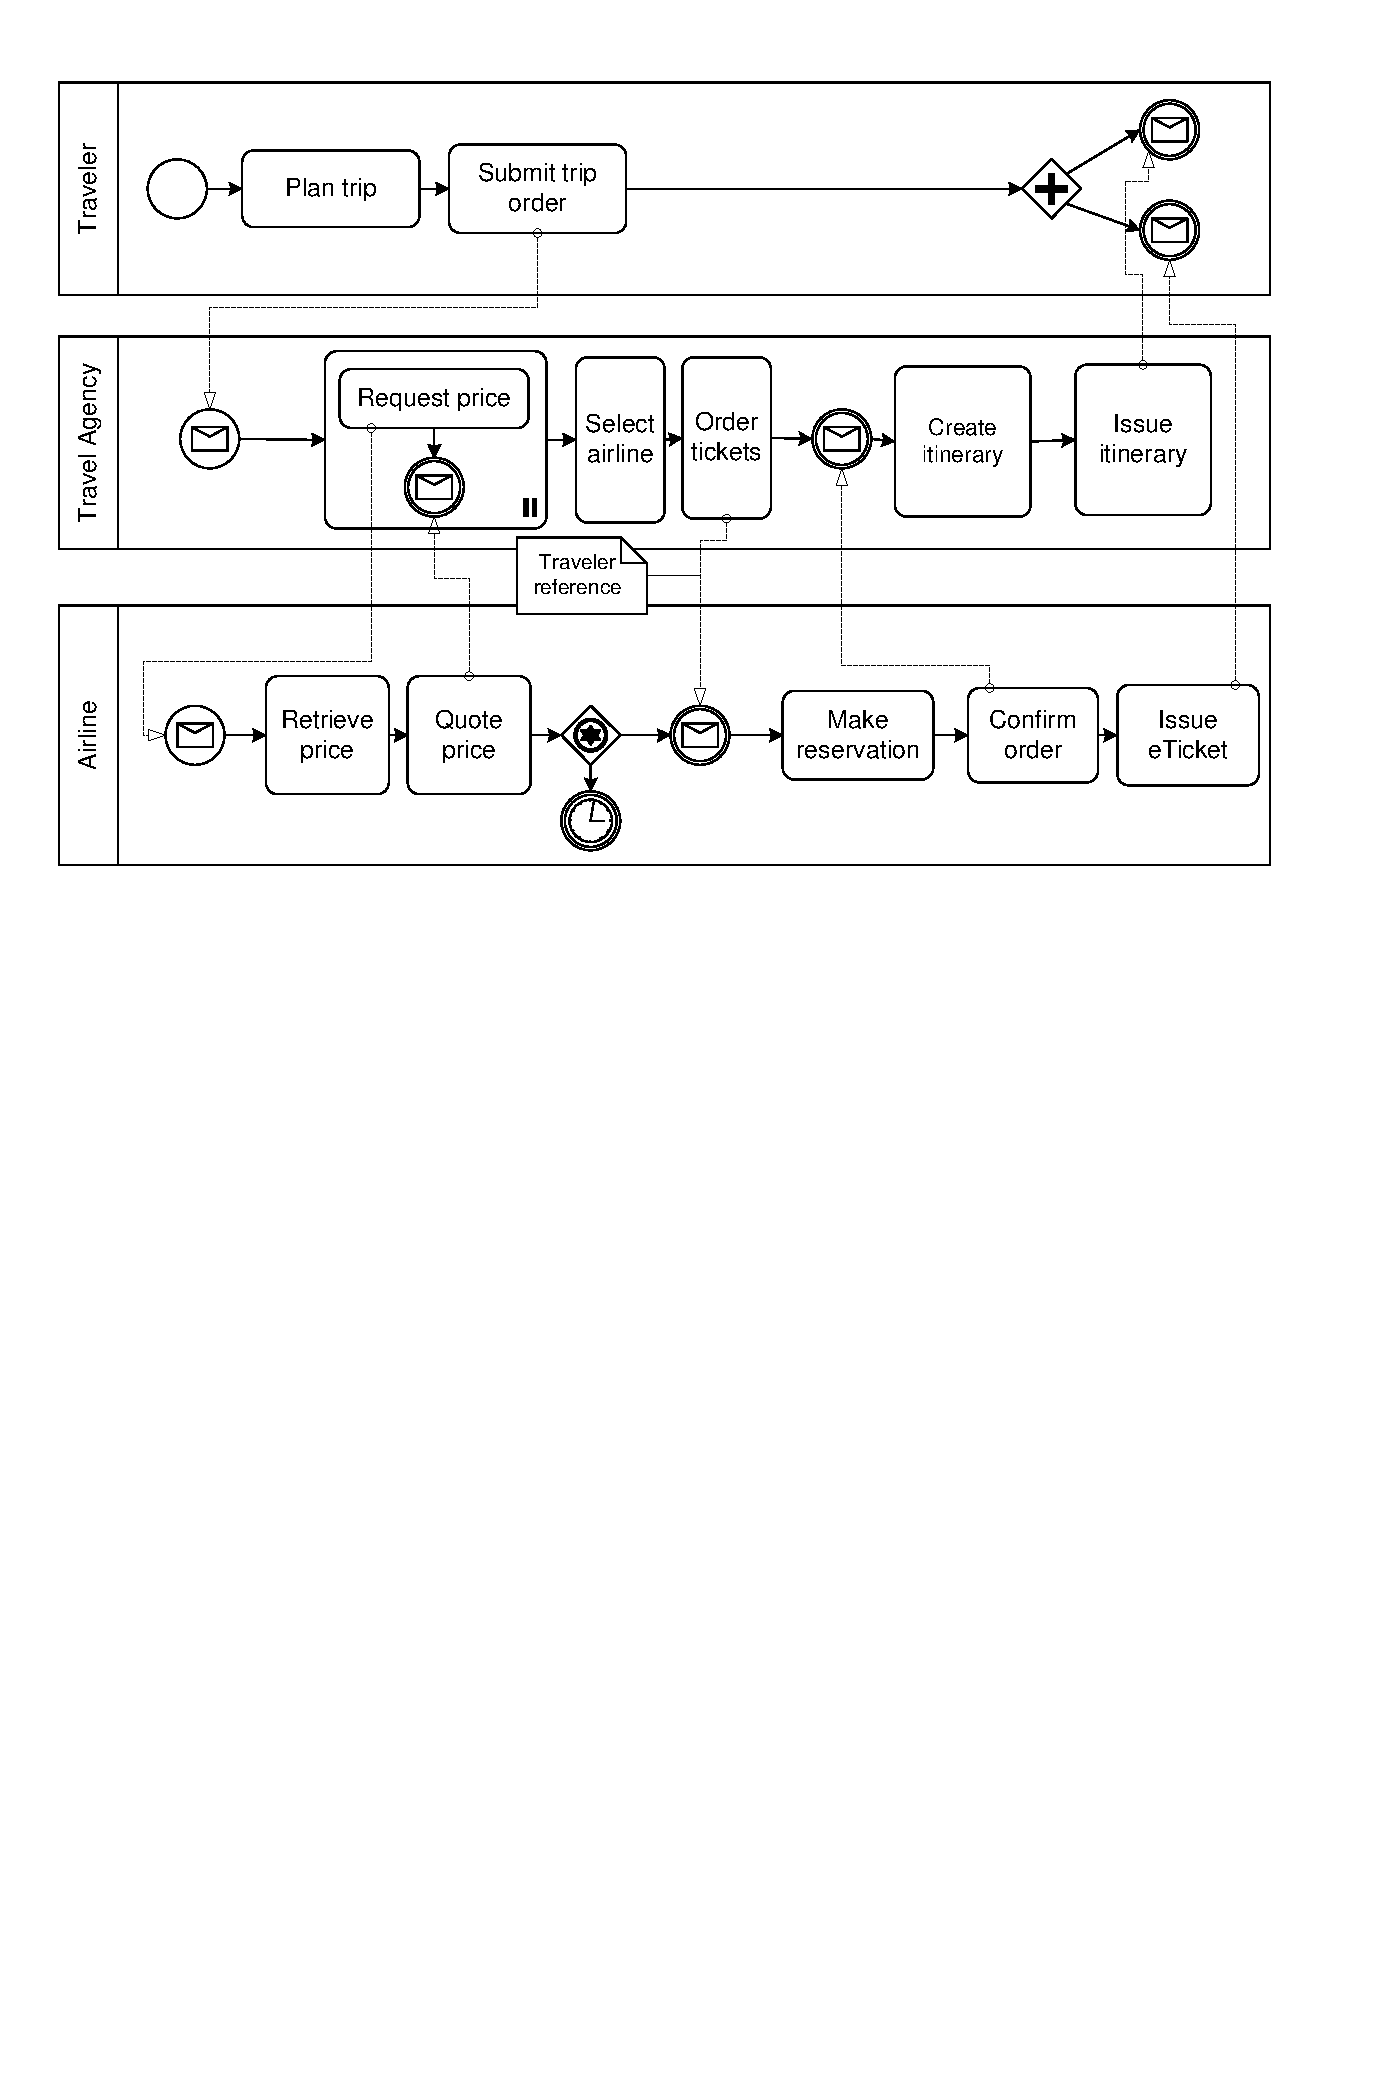
\includegraphics[width=.8\textwidth]{choreography.pdf}
  \caption[Beispiel-Choreographie]{Die Beispiel-Choreographie.
    Nun etwas kleiner, damit \texttt{\textbackslash textwidth} demonstriert wird.
    Und auch die Verwendung von alternativen Bildunterschriften für das Verzeichnis der Abbildungen.
    Letzteres ist allerdings nur Bedingt zu empfehlen, denn wer liest schon so viel Text unter einem Bild?
    Oder ist es einfach nur Stilsache?
  }
  \label{fig:chor2}
\end{figure}


\begin{figure}
  \hfill
  \begin{subfigure}{.3\textwidth}
    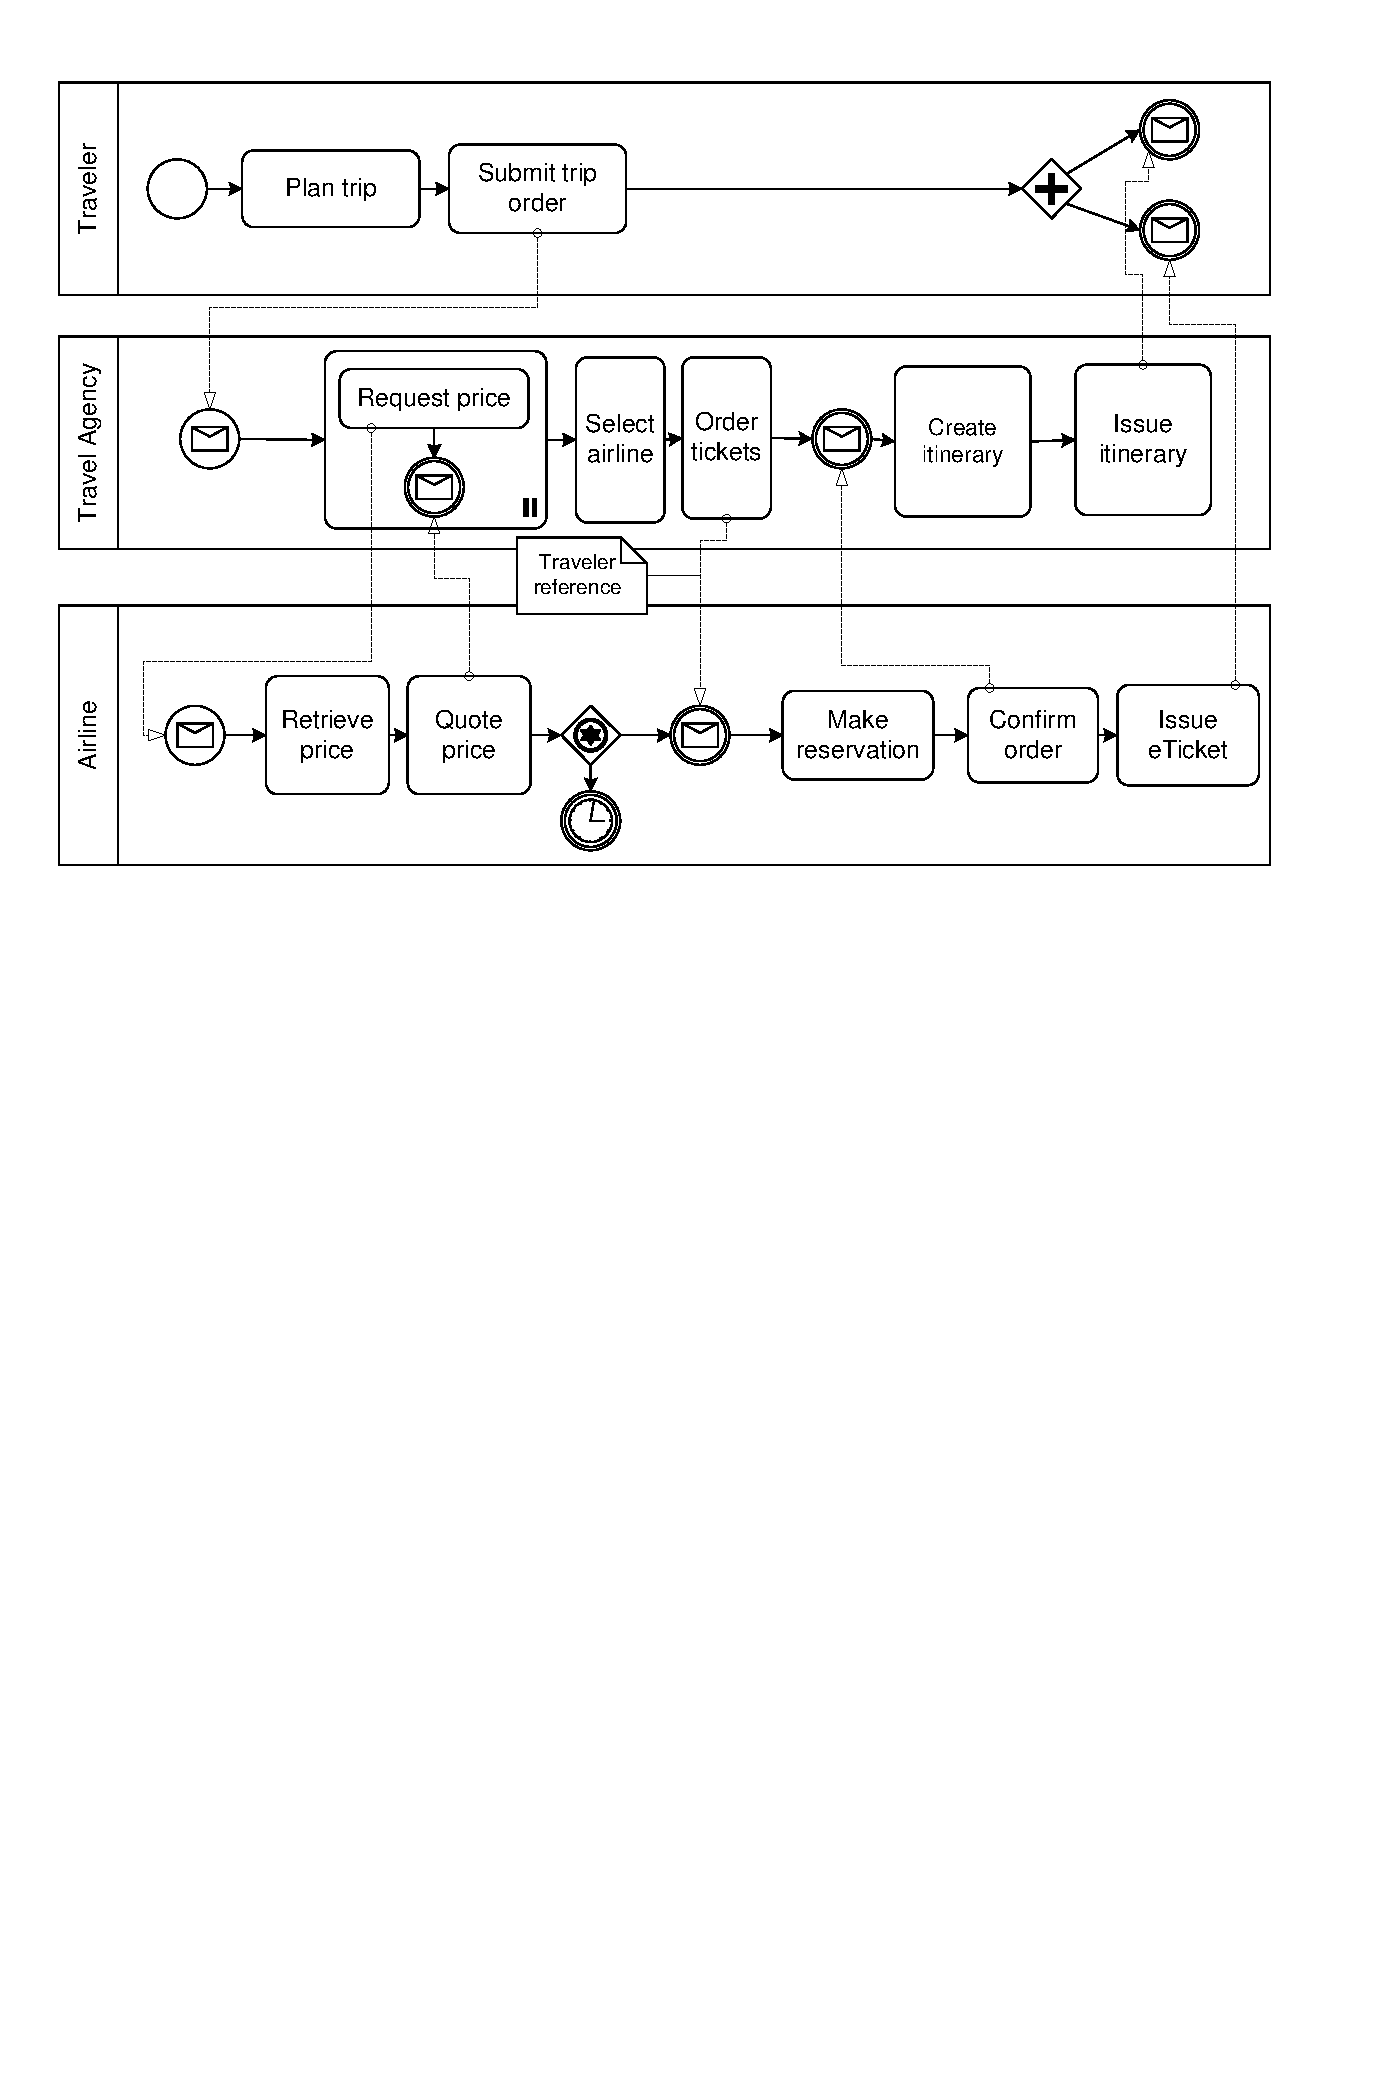
\includegraphics[width=\textwidth]{choreography.pdf}
    \caption{Choreografie 1}
    \label{fig:subfigA}
  \end{subfigure}
  \hfill
  \begin{subfigure}{.3\textwidth}
    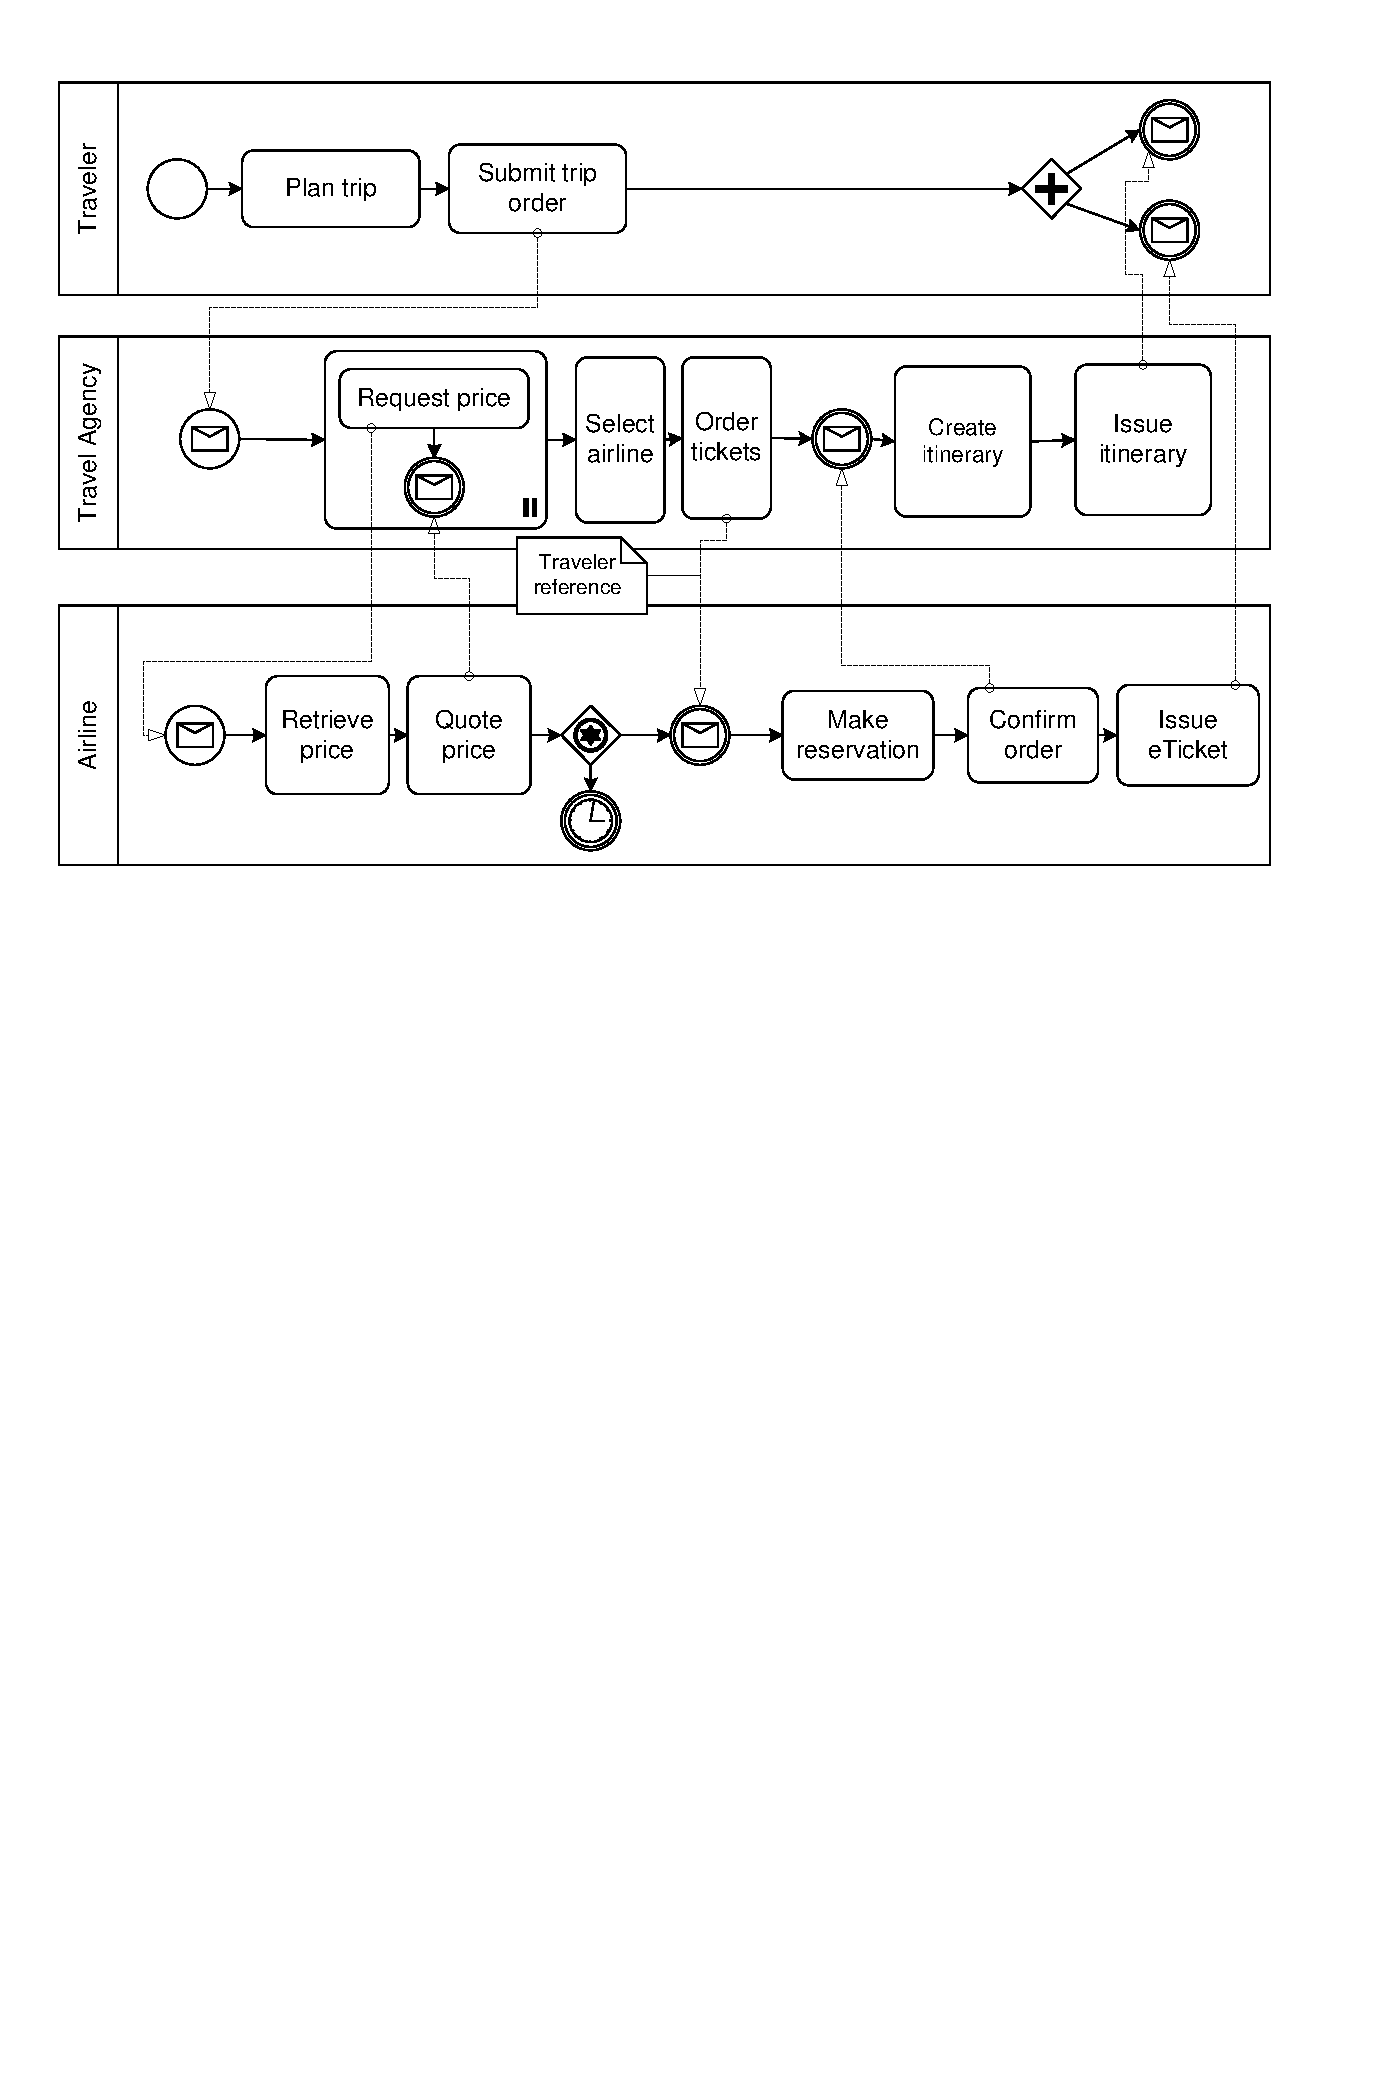
\includegraphics[width=\textwidth]{choreography.pdf}
    \caption{Choreografie 2}
    \label{fig:subfigB}
  \end{subfigure}
  \hfill
  \begin{subfigure}{.3\textwidth}
    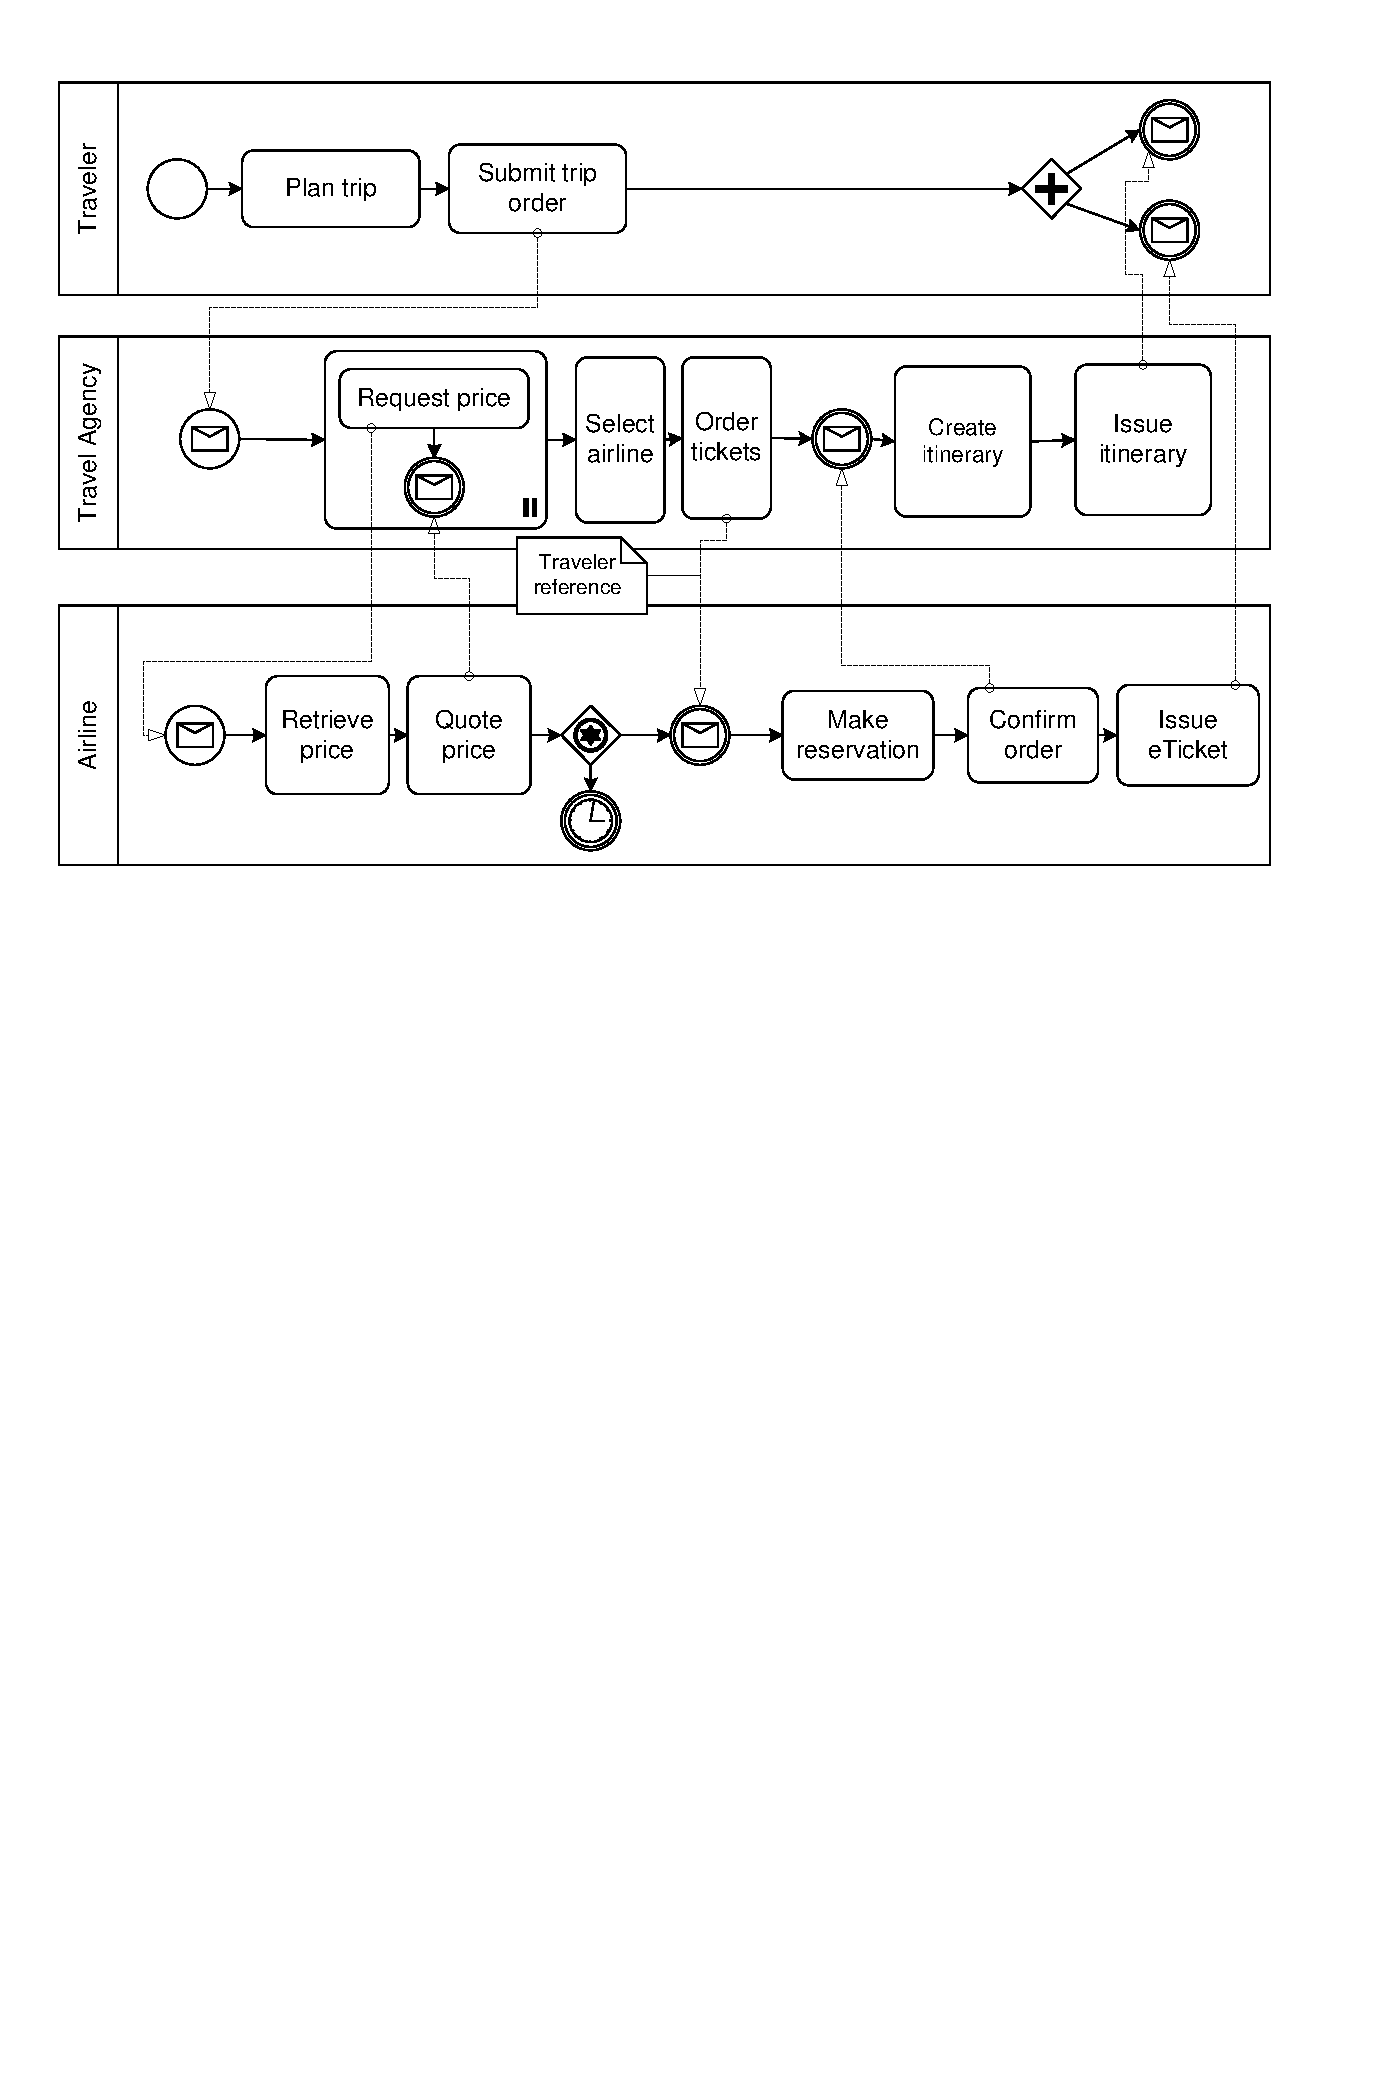
\includegraphics[width=.9\textwidth]{choreography.pdf}
    \caption{Choreografie 3}
    \label{fig:subfigC}
  \end{subfigure}
  \caption{Beispiel um 3 Abbildung nebeneinader zu stellen nur jedes einzeln referenzieren zu können.}
  \label{fig:subfig_example}
\end{figure}

\Cref{fig:subfig_example} zeigt die Verwendung des subcaption-Pakets.
Es ist auch möglich, auf Unterabbildungen zu verweisen: \Cref{fig:subfigA}.

Es ist möglich, SVGs direkt beim Kompilieren in PDF umzuwandeln.
Dies ist im Quellcode zu latex-tipps.tex beschrieben, allerdings auskommentiert.

\iffalse % <-- Das hier wegnehmen, falls inkscape im Pfad ist
  Das SVG in \cref{fig:directSVG} ist direkt eingebunden, während der Text im SVG in \cref{fig:latexSVG} mittels pdflatex gesetzt ist.
  Falls man die Graphiken sehen möchte, muss inkscape im PATH sein und im Tex-Quelltext \texttt{\textbackslash{}iffalse} und \texttt{\textbackslash{}iftrue} auskommentiert sein.

  \begin{figure}
    \centering
    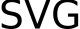
\includegraphics{svgexample.svg}
    \caption{SVG direkt eingebunden}
    \label{fig:directSVG}
  \end{figure}

  \begin{figure}
    \centering
    \def\svgwidth{.4\textwidth}
    \includesvg{svgexample}
    \caption{Text im SVG mittels \LaTeX{} gesetzt}
    \label{fig:latexSVG}
  \end{figure}
\fi % <-- Das hier wegnehmen, falls inkscape im Pfad ist


\section{Weitere Illustrationen}
\Cref{fig:AnhangsChor,fig:AnhangsChor2} zeigen zwei Choreographien, die den Sachverhalt weiter erläutern sollen.
Die zweite Abbildung ist um 90 Grad gedreht, um das Paket \texttt{pdflscape} zu demonstrieren.

\begin{figure}
  \centering
  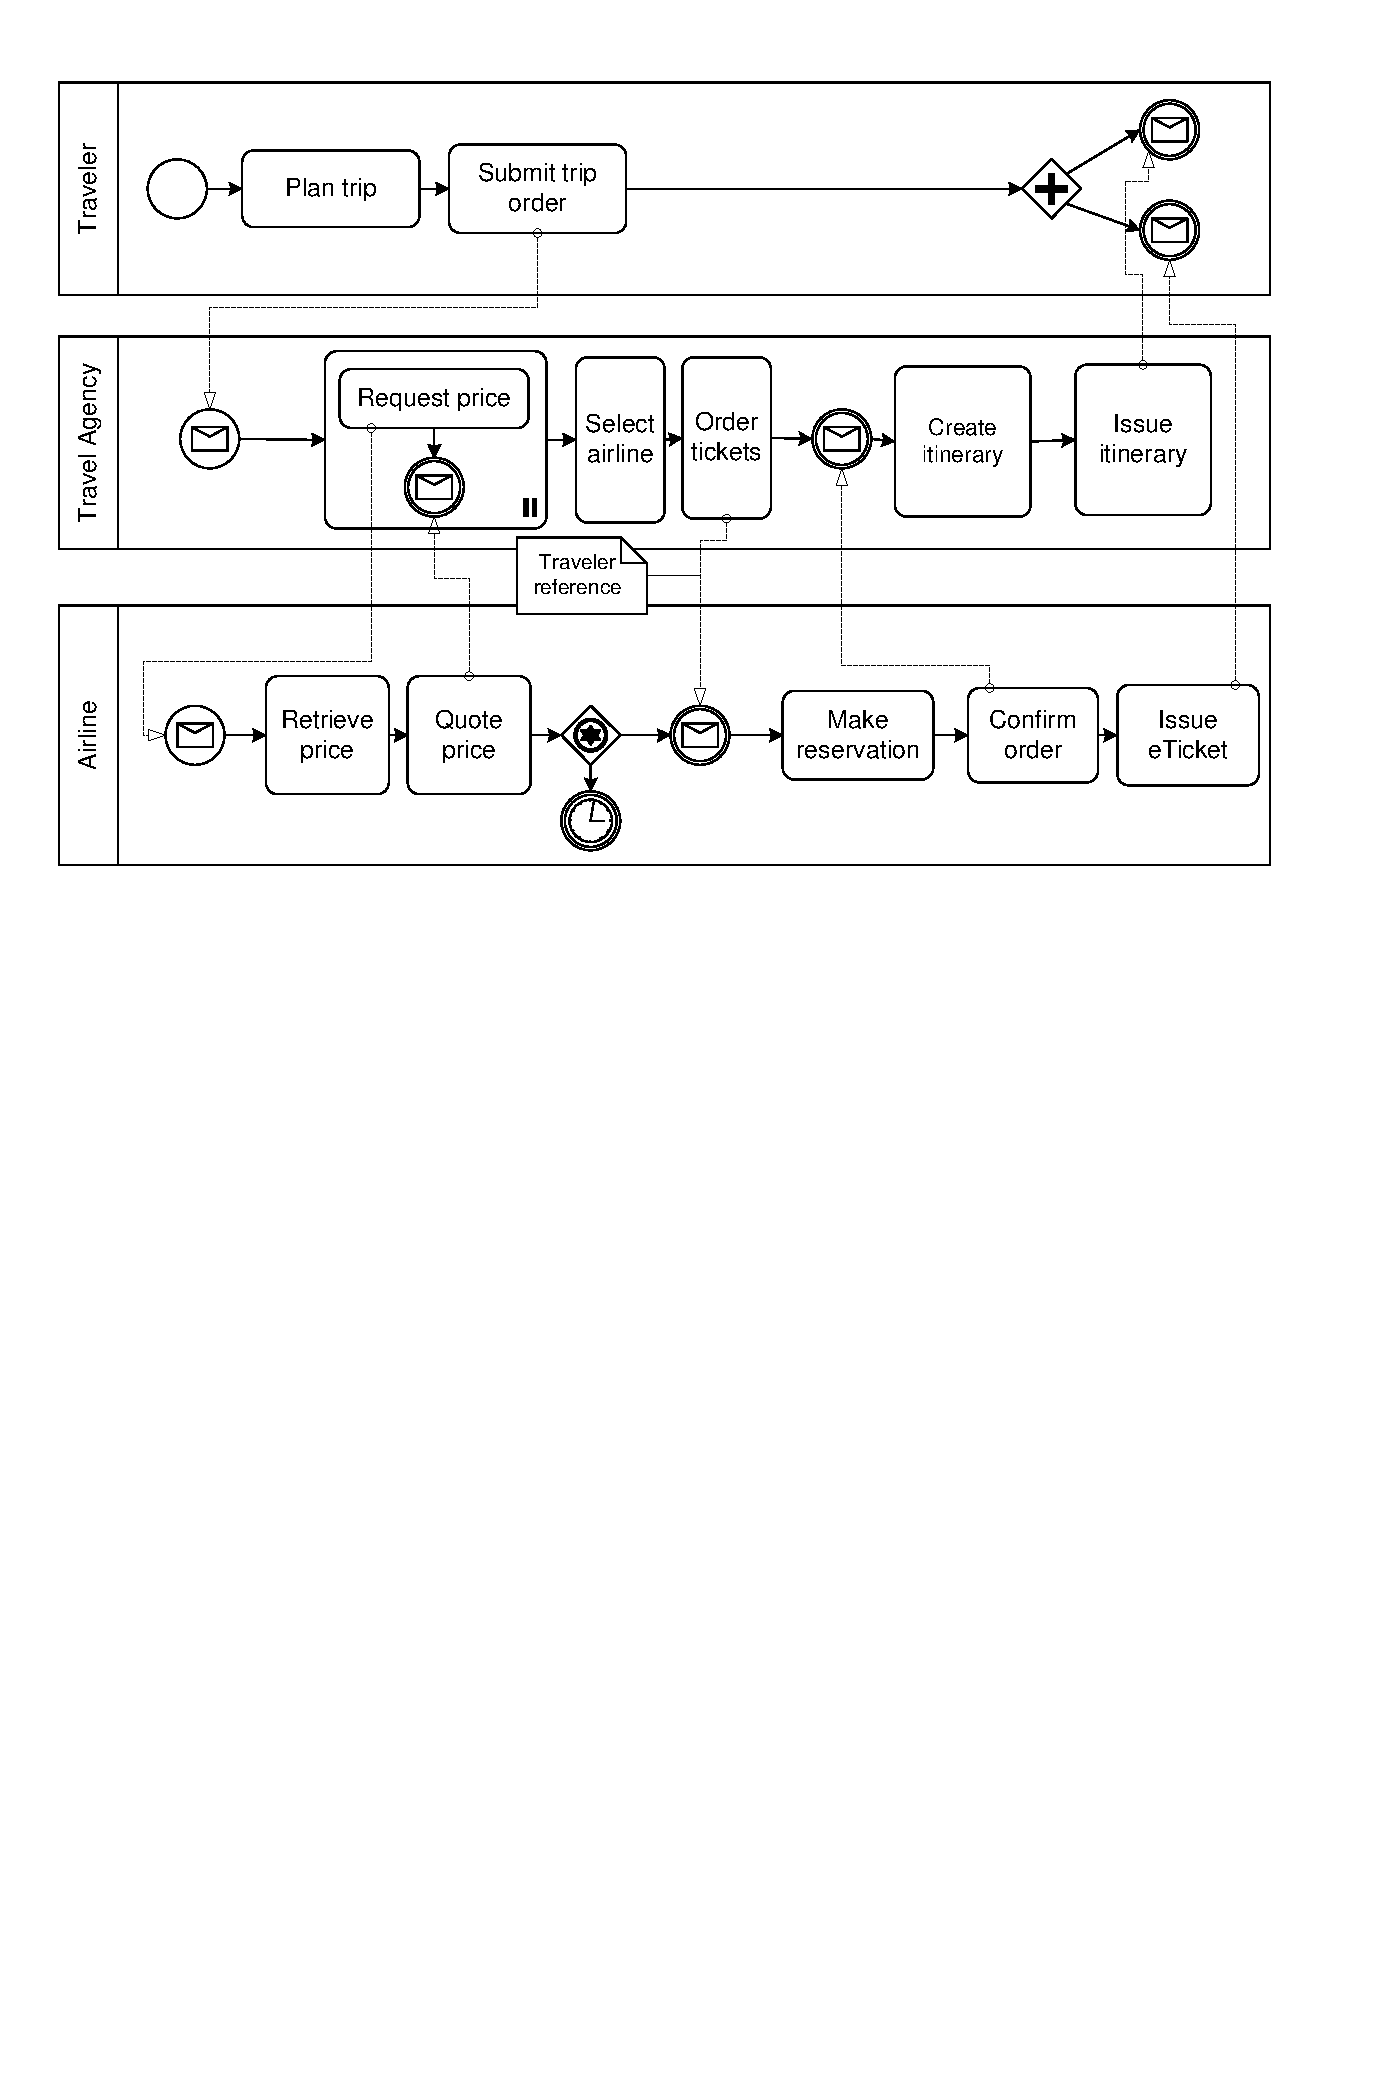
\includegraphics[width=\textwidth]{choreography.pdf}
  \caption{Beispiel-Choreographie I}
  \label{fig:AnhangsChor}
\end{figure}

\begin{landscape}
  \begin{figure}
    \centering
    \includegraphics[width=\textwidth]{choreography.pdf}
    \caption{Beispiel-Choreographie II}
    \label{fig:AnhangsChor2}
  \end{figure}
\end{landscape}


\iffalse

  \clearpage

  FIXME - This does not work with MiKTeX as of 2016-12-30

  TODO- demonstrate rotating package

  %hint by http://tex.stackexchange.com/a/3265/9075
  %other option is to use changepage according to http://tex.stackexchange.com/a/2639/9075. This, however, has issues with landscape
  \thispagestyle{empty}

  \savegeometry{koma}

  %If you only have height problems, this is not needed at all
  \addtolength{\textwidth}{2cm}
  \addtolength{\evensidemargin}{-1cm}

  \begin{landscape}
    %sidewaysfigure
    \begin{figure}
      \centering
      \includegraphics[width=0.9\paperheight]{choreography.pdf}
      \caption{Beispiel-Choreographie, auf einer weißen Seite gezeigt wird und über die definierten Seitenränder herausragt}
    \end{figure}
  \end{landscape}

  %the original layout is restored.
  %%\restoregeometry cannot be used as we use \addtolength
  \loadgeometry{koma}

\fi

\IfFileExists{pgfplots.sty}{
  \section{Plots with pgfplots}
  Pgfplot ist ein Paket um Graphen zu plotten ohne den Umweg über gnuplot oder matplotlib zu gehen.
  %hint by http://tex.stackexchange.com/a/3265/9075%other option is to use changepage according to http://tex.stackexchange.com/a/2639/9075. This, however, has issues with landscape%If you only have height problems, this is not needed at all%sidewaysfigure%the original layout is restored.%%\restoregeometry cannot be used as we use \addtolength
  \begin{figure}[h]
    \begin{center}
      \begin{tikzpicture}
        \begin{axis}[xlabel=$x$,
            ylabel=$\sin(x)$]
          \addplot {sin(deg(x))};  % Sinus-Funktion zeichnen
        \end{axis}
      \end{tikzpicture}
    \end{center}
    \caption{$\sin(x)$ mit pgfplots.}
  \end{figure}

   \begin{figure}[h]
    \begin{center}
      \begin{tikzpicture}
        \begin{axis}[xlabel=$x$,
            ylabel=$y$]
          \addplot table [x=a, y=c, col sep=comma] {data/data.csv};  % Koordinaten aus einer CSV-Datei lesen und plotten
        \end{axis}
      \end{tikzpicture}
    \end{center}
    \caption{Koordianten $x$ und $y$ aus einer CSV-Datei geplottet mit pgfplots.}
  \end{figure}

}{}

\section{Figures with tikz}
TikZ ist ein Paket um Zeichnungen mittels Programmierung zu erstellen.
Dieses Paket eignet sich um Gitter zu erstellen oder andere regelmäßige Strukturen zu erstellen.
Hier gibt es sehr viele visuelle Beispiele was tikz alles kann\footnote{\url{http://texdoc.net/pkg/visualtikz}}.

\begin{figure}[ht]
  \begin{center}
    \begin{tikzpicture}
      \draw(0,0) rectangle (4,4);
      \foreach \x in {0.5,1,1.5,2,2.5,3,3.5}
      \foreach \y in {0.5,1,1.5,2,2.5,3,3.5}
      \draw(\x,\y) circle (1pt);
    \end{tikzpicture}
  \end{center}
  \caption{Eine tikz-Graphik.}\label{fig:tikz_example}
\end{figure}


\section{UML-Diagramme mit tikz-uml}

\Cref{fig:uml} zeigt ein Klassendiagramm, das mittels tikz-uml gesetzt wurde.

\begin{center}
\begin{figure}
\begin{tikzpicture}
\begin{umlpackage}{p}
\begin{umlpackage}{sp1}
\umlclass[template=T]{A}{
  n : uint \\ t : float
}{}
\umlclass[y=-3]{B}{
  d : double
}{
  \umlvirt{setB(b : B) : void} \\ getB() : B}
\end{umlpackage}
\begin{umlpackage}[x=10,y=-6]{sp2}
\umlinterface{C}{
  n : uint \\ s : string
}{}
\end{umlpackage}
\umlclass[x=2,y=-10]{D}{
  n : uint
  }{}
\end{umlpackage}

\umlassoc[geometry=-|-, arg1=tata, mult1=*, pos1=0.3, arg2=toto, mult2=1, pos2=2.9, align2=left]{C}{B}
\umlunicompo[geometry=-|, arg=titi, mult=*, pos=1.7, stereo=vector]{D}{C}
\umlimport[geometry=|-, anchors=90 and 50, name=import]{sp2}{sp1}
\umlaggreg[arg=tutu, mult=1, pos=0.8, angle1=30, angle2=60, loopsize=2cm]{D}{D}
\umlinherit[geometry=-|]{D}{B}
\umlnote[x=2.5,y=-6, width=3cm]{B}{Eine Notiz f\"ur die Klasse B}
\umlnote[x=7.5,y=-2]{import-2}{Eine Anmerkung}
\end{tikzpicture}
\caption{Ein Klassendiagramm mit tikz-uml generiert. Beispiel von Nicolas Kielbasiewicz adaptiert.}
\label{fig:uml}
\end{figure}
\end{center}

\section{Tabellen}

\cref{tab:Ergebnisse} zeigt Ergebnisse und die \cref{tab:Ergebnisse} zeigt wie numerische Daten in einer Tabelle representiert werden können.
\begin{table}
  \centering
  \begin{tabular}{ccc}
    \toprule
    \multicolumn{2}{c}{\textbf{zusammengefasst}} & \textbf{Titel}                                                          \\ \midrule
    Tabelle                                      & wie                                                           & in      \\
    \url{tabsatz.pdf}                            & empfohlen                                                     & gesetzt \\

    \multirow{2}{*}{Beispiel}                    & \multicolumn{2}{c}{ein schönes Beispiel}                                \\
                                                 & \multicolumn{2}{c}{für die Verwendung von \qq{multirow}}           \\
    \bottomrule
  \end{tabular}
  \caption[Beispieltabelle]{Beispieltabelle -- siehe \url{http://www.ctan.org/tex-archive/info/german/tabsatz/}}
  \label{tab:Ergebnisse}
\end{table}

\begin{table}
  \centering
  \begin{tabular}{l *{8}{d{3.2}}}
    \toprule

                         & \multicolumn{2}{c}{\textbf{Parameter 1}} & \multicolumn{2}{c}{\textbf{Parameter 2}} & \multicolumn{2}{c}{\textbf{Parameter 3}} & \multicolumn{2}{c}{\textbf{Parameter 4}}                                                                                                                                       \\
    \cmidrule(r){2-3}\cmidrule(lr){4-5}\cmidrule(lr){6-7}\cmidrule(l){8-9}

    \textbf{Bedingungen} & \multicolumn{1}{c}{\textbf{M}}           & \multicolumn{1}{c}{\textbf{SD}}          & \multicolumn{1}{c}{\textbf{M}}           & \multicolumn{1}{c}{\textbf{SD}}          & \multicolumn{1}{c}{\textbf{M}} & \multicolumn{1}{c}{\textbf{SD}} & \multicolumn{1}{c}{\textbf{M}} & \multicolumn{1}{c}{\textbf{SD}} \\
    \midrule

    W                    & 1.1                                      & 5.55                                     & 6.66                                     & .01                                      &                                &                                 &                                &                                 \\
    X                    & 22.22                                    & 0.0                                      & 77.5                                     & .1                                       &                                &                                 &                                &                                 \\
    Y                    & 333.3                                    & .1                                       & 11.11                                    & .05                                      &                                &                                 &                                &                                 \\
    Z                    & 4444.44                                  & 77.77                                    & 14.06                                    & .3                                       &                                &                                 &                                &                                 \\
    \bottomrule
  \end{tabular}

  \caption{
    Beispieltabelle f\"{u}r 4 Bedingungen (W-Z) mit jeweils 4 Parameters mit (M und SD).
    Hinweis: Stets die selbe Anzahl an Nachkommastellen angeben.
  }
  \label{tab:Werte}
\end{table}



\IfFileExists{pgfplotstable.sty}{

\subsection{Tabellen mit pgfplots}
Mit pgfplots koennen Tabellen direkt aus einer CSV-Datei erstellt werden.

\begin{table}[h]
\centering
\pgfplotstabletypeset[
col sep = comma,
every head row/.style={before row=\toprule,after row=\midrule},
every last row/.style={after row=\bottomrule},
display columns/0/.style={string type,column name={}}
]
{data/data.csv}
\caption{Tabelle generiert aus einer CSV-Datei mit pgfplots}
\end{table}
}{}


\section{Tabellen über mehere Seiten}

\begin{longtable}{|l|l|l|}
\caption{Tabelle \"uber mehere Seiten} \label{tab:long} \\

\hline \multicolumn{1}{|c|}{\textbf{A}} & \multicolumn{1}{c|}{\textbf{B}} & \multicolumn{1}{c|}{\textbf{B}} \\ \hline
\endfirsthead

\multicolumn{3}{c}%
{{\bfseries \tablename\ \thetable{} -- von dor vorherigen Seite weitergeführt}} \\
\hline \multicolumn{1}{|c|}{\textbf{First column}} & \multicolumn{1}{c|}{\textbf{Second column}} & \multicolumn{1}{c|}{\textbf{Third column}} \\ \hline
\endhead

\hline \multicolumn{3}{|r|}{{Wird auf der n\"achsten Seite fortgef\"uhrt}} \\ \hline
\endfoot

\hline \hline
\endlastfoot

A & B C & D \\
A & B C & D \\
A & B C & D \\
A & B C & D \\
A & B C & D \\
A & B C & D \\
A & B C & D \\
A & B C & D \\
A & B C & D \\
A & B C & D \\
A & B C & D \\
A & B C & D \\
A & B C & D \\
A & B C & D \\
A & B C & D \\
A & B C & D \\
A & B C & D \\
A & B C & D \\
A & B C & D \\
A & B C & D \\
A & B C & D \\
A & B C & D \\
A & B C & D \\
A & B C & D \\
A & B C & D \\
A & B C & D \\
A & B C & D \\
A & B C & D \\
A & B C & D \\
A & B C & D \\
A & B C & D \\
A & B C & D \\
A & B C & D \\
A & B C & D \\
A & B C & D \\
A & B C & D \\
A & B C & D \\
A & B C & D \\
A & B C & D \\
A & B C & D \\
A & B C & D \\
A & B C & D \\
A & B C & D \\
A & B C & D \\
A & B C & D \\
A & B C & D \\
A & B C & D \\
A & B C & D \\
A & B C & D \\
A & B C & D \\
A & B C & D \\
A & B C & D \\
A & B C & D \\
A & B C & D \\
A & B C & D \\
A & B C & D \\
A & B C & D \\
A & B C & D \\
A & B C & D \\
A & B C & D \\
A & B C & D \\
A & B C & D \\
A & B C & D \\
A & B C & D \\
A & B C & D \\
A & B C & D \\
A & B C & D \\
A & B C & D \\
A & B C & D \\
A & B C & D \\
A & B C & D \\
A & B C & D \\
A & B C & D \\
A & B C & D \\
A & B C & D \\
A & B C & D \\
A & B C & D \\
A & B C & D \\
A & B C & D \\
A & B C & D \\
\end{longtable}


\section{Abkürzungen}

Beim ersten Durchlauf betrug die \gls{fr} 5.
Beim zweiten Durchlauf war die \gls{fr} 3.
Die Pluralform sieht man hier: \glspl{er}.
Um zu demonstrieren, wie das Abkürzungsverzeichnis bei längeren Beschreibungstexten aussieht, muss hier noch \glspl{rdbms} erwähnt werden.

Mit \verb+\gls{...}+ können Abkürzungen eingebaut werden, beim ersten Aufrufen wird die lange Form eingesetzt.
Beim wiederholten Verwenden von \verb+\gls{...}+ wird automatisch die kurz Form angezeigt.
Außerdem wird die Abkürzung automatisch in die Abkürzungsliste eingefügt.
Mit \verb+\glspl{...}+ wird die Pluralform verwendet.
Möchte man, dass bei der ersten Verwendung direkt die Kurzform erscheint, so kann man mit \verb+\glsunset{...}+ eine Abkürzung als bereits verwendet markieren.
Das Gegenteil erreicht man mit \verb+\glsreset{...}+.

Definiert werden Abkürzungen in der Datei \textit{content\\ausarbeitung.tex} mithilfe von \verb+\newacronym{...}{...}{...}+.

Mehr Infos unter: \url{http://tug.ctan.org/macros/latex/contrib/glossaries/glossariesbegin.pdf}


\section{Verweise}
Für weit entfernte Abschnitte ist \qq{varioref} zu empfehlen:
\qq{Siehe \vref{sec:mf}}.
Das Kommando \texttt{\textbackslash{}vref} funktioniert ähnlich wie \texttt{\textbackslash{}cref} mit dem Unterschied, dass zusätzlich ein Verweis auf die Seite hinzugefügt wird.
\texttt{vref}: \qq{\vref{sec:firstsectioninlatexhints}}, \texttt{cref}: \qq{\cref{sec:firstsectioninlatexhints}}, \texttt{ref}: \qq{\ref{sec:firstsectioninlatexhints}}.

Falls \qq{varioref} Schwierigkeiten macht, dann kann man stattdessen \qq{cref} verwenden.
Dies erzeugt auch das Wort \qq{Abschnitt} automatisch: \cref{sec:mf}.
Das geht auch für Abbildungen usw.
Im Englischen bitte \verb1\Cref{...}1 (mit großem \qq{C} am Anfang) verwenden.


%Mit MiKTeX Installation ab dem 2012-01-16 nicht mehr nötig
%Falls ein Abschnitt länger als eine Seite wird und man mittels \texttt{\textbackslash{}vref} auf eine konkrete Stelle in der Section
%verweisen möchte, dann sollte man \texttt{\textbackslash{}phantomsection} verwenden und dann wird
%auch bei \texttt{vref} die richtige Seite angeben.

%%The link location will be placed on the line below.
%%Tipp von http://en.wikibooks.org/wiki/LaTeX/Labels_and_Cross-referencing#The_hyperref_package_and_.5Cphantomsection
%\phantomsection
%\label{alabel}
%Das Beispiel für \texttt{\textbackslash{}phantomsection} bitte im \LaTeX{}-Quellcode anschauen.

%Hier das Beispiel: Siehe Abschnitt \vref{hack1} und Abschnitt \vref{hack2}.


\section{Definitionen}
\begin{definition}[Title]
  \label{def:def1}
  Definition Text
\end{definition}

\Cref{def:def1} zeigt \ldots

\section{Fußnoten}
Fußnoten können mit dem Befehl \verb+\footnote{...}+ gesetzt werden\footnote{\label{fussnote}Diese Fußnote ist ein Beispiel.
}.
Mehrfache Verwendung von Fußnoten ist möglich indem man zu erst ein Label in der Fußnote setzt \verb+\footnote{\label{...}...}+ und anschließend mittels \verb+\cref{...}+ die Fußnote erneut verwendet\cref{fussnote}.


\section{Verschiedenes}
\label{sec:diff}
\ifdeutsch
  Ziffern (123\,654\,789) werden schön gesetzt.
  Entweder in einer Linie oder als Minuskel-Ziffern.
  Letzteres erreicht man durch den Parameter \texttt{osf} bei dem Paket \texttt{libertine} bzw.\ \texttt{mathpazo} in \texttt{fonts.tex}.
\fi

\begin{compactenum}[I.]
  \item Man kann auch die Nummerierung dank paralist kompakt halten
  \item und auf eine andere Nummerierung umstellen
\end{compactenum}

Die Wörter \qq{Workflow} und \qq{Auflage} lassen sich im PDF kopieren und in eine Textdatei einfügen.

Bei der Nutzung von \LuaLaTeX{} wird bei \qq{Auflage} automatisch keine Ligatur bei \qq{f\/l} (im Gegensatz zu \qq{fl} bei \qq{workflow}) gesetzt.
In anderen Worten: \qq{Auflage} und \qq{Auf\/lage} sehen im Falle der Nutzung von \LuaLaTeX{} im PDF gleich aus.
Weiterhin setzt dieses Vorgehen die Duden-Regeln bezüglich \qq{Ligaturen} \cite[S.\ 96]{Duden2001} um.

\section{Schlusswort}
Verbesserungsvorschläge für diese Vorlage sind immer willkommen.
Bitte bei GitHub ein Ticket eintragen (\url{https://github.com/latextemplates/scientific-thesis-template/issues}).


\pagestyle{empty}
\renewcommand*{\chapterpagestyle}{empty}
\Versicherung
\end{document}
